\documentclass{report}
\usepackage[utf8]{inputenc}
\usepackage[T5]{fontenc}
\usepackage[fontsize=13pt]{scrextend}
\usepackage[hidelinks]{hyperref}
\usepackage{amsmath}
\usepackage[vietnamese]{babel}
\usepackage[paperheight=29.7cm, paperwidth=21cm, top=2cm, bottom=2cm, left=2.5cm, right=2.5cm]{geometry} % Đảm bảo cân đối lề
\usepackage{times} % Chọn font Time New Roman
\usepackage{graphicx} % Required for inserting images
\usepackage{float}
\usepackage{tikz}
\usetikzlibrary{calc}
\renewcommand{\thesection}{\Roman{section}}
\renewcommand{\thesubsection}{\arabic{subsection}}
\renewcommand{\thesubsubsection}{\thesubsection.\arabic{subsubsection}}
\definecolor{dkgreen}{rgb}{0,0.6,0}
\definecolor{gray}{rgb}{0.5,0.5,0.5}
\definecolor{mauve}{rgb}{0.58,0,0.82}
\usepackage{listings}
\usepackage[most]{tcolorbox}

\setcounter{secnumdepth}{3}
\renewcommand{\thesubsubsection}{\thesubsection.\arabic{subsubsection}}

\usepackage{booktabs}
\usepackage{colortbl} % Cần thiết để đổi màu đường kẻ \arrayrulecolor
\usepackage{xcolor}

\definecolor{lightgray}{RGB}{230, 230, 230}

% Định nghĩa khung xám bo góc
\newtcolorbox{mycodebox}{
  colback=gray!10,       % Màu nền xám nhạt
  colframe=gray!10,      % Viền cùng màu nền
  arc=4pt,               % Bo góc nhẹ
  boxrule=0pt,
  left=12pt, right=12pt, top=10pt, bottom=10pt
}
\usepackage{color} % tô màu cho code
\lstset{frame=tb,
  language=Python,
  aboveskip=3mm,
  belowskip=3mm,
  showstringspaces=false,
  columns=flexible,
  basicstyle={\small\ttfamily},
  numbers=none,
  numberstyle=\tiny\color{gray},
  keywordstyle=\color{blue},
  commentstyle=\color{dkgreen},
  stringstyle=\color{mauve},
  breaklines=true,
  breakatwhitespace=true,
  tabsize=3
}

\begin{document}
\begin{titlepage}

\begin{tikzpicture}[overlay,remember picture]
% Khung ngoài
\draw[line width=3pt]
    ($ (current page.north west) + (2.5cm,-2.5cm) $)
    rectangle
    ($ (current page.south east) + (-2.5cm,2.5cm) $);
% Khung trong
\draw[line width=0.5pt]
    ($ (current page.north west) + (2.6cm,-2.6cm) $)
    rectangle
    ($ (current page.south east) + (-2.6cm,2.6cm) $);
\end{tikzpicture}

\begin{center}
\textbf{\vspace{0.1cm}\fontsize{16pt}{0pt}\selectfont TRƯỜNG ĐẠI HỌC XÂY DỰNG HÀ NỘI}\\
\textbf{\fontsize{16pt}{0pt}\selectfont KHOA CÔNG NGHỆ THÔNG TIN}

\vspace{0.8cm}
\begin{figure}[H]
    \centering
    
\includegraphics[width=2.5cm, height=2.5cm]{Image/911px-LOGO_DHXD.png}
\end{figure}

\vspace{2cm}
\textbf{\fontsize{30pt}{0pt}\selectfont ĐỒ ÁN TỐT NGHIỆP}\\

\vspace{12pt}
\parbox{0.9\textwidth}{
    \centering
    \fontsize{18pt}{22pt}\selectfont
    \textbf{XÂY DỰNG WEBSITE THƯƠNG MẠI ĐIỆN TỬ SẢN PHẨM CÔNG NGHỆ TÍCH HỢP\\TRÍ TUỆ NHÂN TẠO HỖ TRỢ TÌM KIẾM, \\TƯ VẤN VÀ GỢI Ý SẢN PHẨM}
}
\end{center}

\vspace{1.5cm}
\hspace{1.5cm}
\fontsize{14pt}{0pt}\selectfont Giảng viên hướng dẫn: Ths. Lê Văn Minh\\[0.3cm]
\vspace{0.3cm}
\hspace{2cm}
\fontsize{14pt}{0pt}\selectfont Chuyên ngành: Khoa học máy tính \\
\vspace{0.3cm}
\hspace{1.9cm}
\fontsize{14pt}{18pt}\selectfont
Sinh viên thực hiện:\\[-1cm]

\begin{center}
    \renewcommand{\arraystretch}{1.5}
    \begin{tabular}{l @{\hspace{2cm}} c}
        Phạm Hồng Quân   & 0304967 \\
        Nguyễn Đình Sông & 0271067 \\
        Hoàng Văn Tới    & 0233967 \\
    \end{tabular}
\end{center}
\begin{center}
\vspace{2cm}
\fontsize{14pt}{0pt}\selectfont Hà Nội, 08 - 2026
\end{center}
\end{titlepage}
\newpage
\begin{center}
    \fontsize{18pt}{22pt}\selectfont \textbf{LỜI CẢM ƠN}
\end{center}
Trong suốt quá trình học tập và thực hiện đồ án tốt nghiệp, nhóm chúng em đã nhận được sự quan tâm, hướng dẫn và hỗ trợ quý báu từ quý thầy cô, gia đình và bạn bè. Đây là nguồn động viên to lớn giúp nhóm chúng em vượt qua những khó khăn và hoàn thành đồ án.\\ 

Trước hết, nhóm chúng em xin gửi lời cảm ơn chân thành đến \textbf{quý thầy cô Khoa Công nghệ Thông tin} đã tận tình giảng dạy, truyền đạt những kiến thức và kinh nghiệm quý báu trong suốt quá trình học tập. Những kiến thức này là nền tảng quan trọng giúp nhóm chúng em vận dụng vào quá trình nghiên cứu và thực hiện đồ án tốt nghiệp.\\

Đặc biệt, nhóm chúng em xin bày tỏ lòng biết ơn sâu sắc đến \textbf{thầy Lê Văn Minh}, người đã tận tình hướng dẫn, định hướng và đưa ra những ý kiến đóng góp quý báu, giúp nhóm chúng em từng bước giải quyết khó khăn và hoàn thiện đồ án.\\

Bên cạnh đó, nhóm chúng em xin cảm ơn gia đình và bạn bè đã luôn động viên, hỗ trợ và tạo điều kiện thuận lợi trong suốt quá trình học tập và thực hiện đồ án.\\

Mặc dù đã nỗ lực nghiên cứu và hoàn thiện đồ án, nhưng do kiến thức, kinh nghiệm thực tế và thời gian thực hiện còn hạn chế, đồ án khó tránh khỏi những thiếu sót. Nhóm chúng em rất mong nhận được những ý kiến đóng góp từ quý thầy cô để có thể tiếp tục học hỏi và hoàn thiện hơn trong tương lai.\\

Cuối cùng, nhóm chúng em xin kính chúc quý thầy cô luôn dồi dào sức khỏe, hạnh phúc và thành công trong sự nghiệp.\\

Nhóm chúng em xin chân thành cảm ơn!

\newpage
\begin{center}
    \fontsize{18pt}{22pt}\selectfont \textbf{BẢNG PHÂN CHIA CÔNG VIỆC}
\end{center}


\begin{table}[htbp]
    \centering
    \caption{Bảng phân chia công việc của nhóm}
    \label{tab:phan-chia-cong-viec}
    \renewcommand{\arraystretch}{1.4}
    \begin{tabular}{|c|p{3.5cm}|p{8cm}|}
        \hline
        \textbf{STT} &
        \textbf{Thành viên} &
        \textbf{Công việc phụ trách} \\
        \hline

        1 & Nguyễn Đình Sông &
        \textbf{Frontend:} Đảm nhiệm chính việc xây dựng
        giao diện của hệ thống.\newline
        \textbf{Backend:} Xây dựng chức năng đề xuất
        sản phẩm dựa trên hành vi người dùng,
        quên mật khẩu, blog và đánh giá sản phẩm.\newline
        \textbf{AI:} Xây dựng module đề xuất sản phẩm
        dựa trên hành vi người dùng. \\
        \hline

        2 & Phạm Hồng Quân &
        \textbf{Backend:} Đảm nhiệm chính việc xây dựng
        các chức năng nghiệp vụ của hệ thống.\newline
        \textbf{Frontend:} Xây dựng giao diện tìm kiếm
        sản phẩm bằng hình ảnh.\newline
        \textbf{AI:} Xây dựng module tìm kiếm
        sản phẩm bằng hình ảnh. \\
        \hline

        3 & Hoàng Văn Tới &
        \textbf{Backend:} Xây dựng chức năng
        chatbot tư vấn khách hàng.\newline
        \textbf{Frontend:} Xây dựng giao diện chatbot.\newline
        \textbf{AI:} Xây dựng module chatbot
        tư vấn khách hàng.\newline
        \textbf{Dữ liệu:} Thu thập dữ liệu
        phục vụ hệ thống.\newline
        \textbf{Báo cáo:} Viết báo cáo đồ án. \\
        \hline

        4 & Công việc chung &
        Thiết kế hệ thống.\newline
        Thiết kế cơ sở dữ liệu. \\
        \hline

    \end{tabular}
\end{table}


\newpage
\tableofcontents
\newpage
\chapter*{PHẦN MỞ ĐẦU}
\addcontentsline{toc}{chapter}{PHẦN MỞ ĐẦU}

\section{Lý do chọn đề tài}
Sự phát triển của Internet và công nghệ thông tin đã thúc đẩy thương mại điện tử trở thành phương thức mua sắm phổ biến. Đối với các sản phẩm công nghệ như máy tính xách tay, điện thoại, tai nghe, máy ảnh và phụ kiện điện tử, sự đa dạng về mẫu mã, thông số kỹ thuật và mức giá mang đến nhiều lựa chọn nhưng cũng khiến người dùng gặp khó khăn trong việc tìm kiếm, so sánh và lựa chọn sản phẩm phù hợp.\\\\
Hiện nay, phần lớn các website thương mại điện tử sử dụng phương pháp tìm kiếm theo từ khóa và bộ lọc có sẵn. Tuy nhiên, các phương pháp này còn hạn chế khi người dùng chưa xác định rõ nhu cầu, không biết chính xác tên sản phẩm hoặc muốn tìm kiếm thông qua hình ảnh. Việc so sánh nhiều sản phẩm cũng đòi hỏi người dùng dành nhiều thời gian tìm hiểu thông tin.\\\\
Sự phát triển của trí tuệ nhân tạo (AI) mở ra khả năng cải thiện trải nghiệm mua sắm thông qua tìm kiếm bằng hình ảnh, chatbot tư vấn và hệ thống gợi ý sản phẩm. Đặc biệt, việc kết hợp mô hình ngôn ngữ lớn (LLM) với kỹ thuật Retrieval-Augmented Generation (RAG) cho phép chatbot khai thác dữ liệu sản phẩm để đưa ra câu trả lời có cơ sở và hạn chế thông tin không chính xác.\\\\
Xuất phát từ những vấn đề trên, nhóm chúng em lựa chọn đề tài \textbf{``Xây dựng website thương mại điện tử sản phẩm công nghệ tích hợp trí tuệ nhân tạo hỗ trợ tìm kiếm, tư vấn và gợi ý sản phẩm''}. Đề tài hướng đến xây dựng một nền tảng mua sắm trực tuyến tích hợp các chức năng AI nhằm hỗ trợ người dùng tìm kiếm, lựa chọn sản phẩm hiệu quả hơn, đồng thời tạo cơ hội vận dụng kiến thức đã học vào thực tiễn.

\section{Mục tiêu đề tài}
\subsection{Mục tiêu tổng quát}
Nghiên cứu, thiết kế và xây dựng website thương mại điện tử kinh doanh sản phẩm công nghệ, đáp ứng nhu cầu tìm kiếm, quản lý và mua sắm trực tuyến. Đồng thời, tích hợp các chức năng trí tuệ nhân tạo (AI) như chatbot tư vấn ứng dụng Retrieval-Augmented Generation (RAG), tìm kiếm bằng hình ảnh và gợi ý sản phẩm thông minh nhằm nâng cao trải nghiệm người dùng và hỗ trợ lựa chọn sản phẩm phù hợp.

\subsection{Mục tiêu cụ thể}
Để đạt được mục tiêu tổng quát, đề tài tập trung vào các mục tiêu sau:

\begin{itemize}
    \item \textbf{Phân tích và thiết kế hệ thống:} Xác định yêu cầu, thiết kế kiến trúc, cơ sở dữ liệu và giao diện website.
    \item \textbf{Xây dựng website thương mại điện tử:} Phát triển các chức năng quản lý tài khoản, tìm kiếm sản phẩm, giỏ hàng, đặt hàng và theo dõi đơn hàng.
    \item \textbf{Phát triển chatbot RAG:} Kết hợp mô hình ngôn ngữ lớn (LLM) với RAG để tư vấn sản phẩm bằng ngôn ngữ tự nhiên dựa trên dữ liệu hệ thống.
    \item \textbf{Tìm kiếm sản phẩm bằng hình ảnh:} Phân tích hình ảnh đầu vào và truy xuất các sản phẩm có đặc điểm tương đồng.
    \item \textbf{Gợi ý sản phẩm thông minh:} Xây dựng chức năng đề xuất sản phẩm dựa trên dữ liệu sản phẩm và hành vi người dùng.
    \item \textbf{Xây dựng chức năng quản trị:} Quản lý người dùng, danh mục, sản phẩm, đơn hàng và nội dung website.
    \item \textbf{Kiểm thử và đánh giá:} Kiểm tra chức năng, đánh giá kết quả hoạt động và xác định các hạn chế của hệ thống.
\end{itemize}


\section{Đối tượng và phạm vi nghiên cứu}
\subsection{Đối tượng nghiên cứu}
Đề tài tập trung nghiên cứu các công nghệ và phương pháp xây dựng website thương mại điện tử tích hợp trí tuệ nhân tạo, bao gồm:

\begin{itemize}
    \item \textbf{Hệ thống thương mại điện tử:} Các quy trình quản lý sản phẩm, người dùng, giỏ hàng, đơn hàng và thanh toán.
    \item \textbf{Công nghệ phát triển web:} Next.js, Spring Boot, FastAPI và PostgreSQL kết hợp pgvector.
    \item \textbf{Chatbot tư vấn sản phẩm:} Mô hình ngôn ngữ lớn (LLM), Retrieval-Augmented Generation (RAG), embedding và tìm kiếm kết hợp.
    \item \textbf{Tìm kiếm bằng hình ảnh:} Các kỹ thuật trích xuất đặc trưng và tìm kiếm sản phẩm dựa trên độ tương đồng.
    \item \textbf{Hệ thống gợi ý sản phẩm:} Các phương pháp phân tích hành vi và đề xuất sản phẩm phù hợp với người dùng.
\end{itemize}

\subsection{Phạm vi nghiên cứu}
Đề tài tập trung xây dựng website thương mại điện tử kinh doanh các sản phẩm công nghệ như máy tính xách tay, điện thoại, tai nghe, máy ảnh, linh kiện và phụ kiện điện tử.\\\\
Hệ thống bao gồm các chức năng mua sắm trực tuyến, quản lý sản phẩm, tài khoản, giỏ hàng, đơn hàng và thanh toán; đồng thời tích hợp ba chức năng AI chính: chatbot tư vấn ứng dụng RAG, tìm kiếm bằng hình ảnh và gợi ý sản phẩm theo hành vi người dùng.\\\\
Dữ liệu phục vụ các chức năng AI được khai thác từ cơ sở dữ liệu sản phẩm của hệ thống. Đề tài được triển khai và đánh giá trong môi trường thử nghiệm, chưa tập trung vào vận hành thương mại quy mô lớn hoặc tối ưu hóa cho số lượng người dùng đồng thời cao.

\section{Phương pháp nghiên cứu}
Để thực hiện đề tài, nhóm sử dụng các phương pháp nghiên cứu sau:

\begin{itemize}
    \item \textbf{Nghiên cứu tài liệu:} Tìm hiểu các công nghệ phát triển web, mô hình ngôn ngữ lớn, RAG, tìm kiếm hình ảnh và hệ thống gợi ý sản phẩm.
    \item \textbf{Phân tích và thiết kế:} Xác định yêu cầu, thiết kế kiến trúc hệ thống, cơ sở dữ liệu và các chức năng nghiệp vụ.
    \item \textbf{Thu thập và xử lý dữ liệu:} Thu thập, làm sạch và chuẩn hóa dữ liệu sản phẩm phục vụ website và các chức năng AI.
    \item \textbf{Thực nghiệm và đánh giá:} Xây dựng, tích hợp, kiểm thử các chức năng và đánh giá kết quả hoạt động của hệ thống.
\end{itemize}

\section{Ý nghĩa của đề tài}
Đề tài góp phần ứng dụng trí tuệ nhân tạo vào thương mại điện tử nhằm hỗ trợ người dùng tìm kiếm, tư vấn và lựa chọn sản phẩm công nghệ phù hợp. Việc tích hợp chatbot RAG, tìm kiếm bằng hình ảnh và hệ thống gợi ý sản phẩm giúp nâng cao khả năng tương tác và trải nghiệm mua sắm trực tuyến.\\\\
Bên cạnh đó, đề tài tạo cơ hội vận dụng kiến thức về phát triển ứng dụng web, cơ sở dữ liệu và trí tuệ nhân tạo vào thực tiễn, đồng thời làm cơ sở để nghiên cứu, cải tiến và mở rộng các chức năng thông minh trong tương lai.

\chapter{CƠ SỞ LÝ THUYẾT}
\section{Tổng quan về thương mại điện tử}
\subsection{Khái niệm và đặc điểm thương mại điện tử}
Thương mại điện tử (Electronic Commerce -- E-commerce) là hình thức thực hiện các hoạt động mua bán hàng hóa và dịch vụ thông qua phương tiện điện tử, chủ yếu là Internet. Các hoạt động bao gồm giới thiệu sản phẩm, tìm kiếm thông tin, đặt hàng, thanh toán và quản lý giao dịch.\\\\
So với thương mại truyền thống, thương mại điện tử cho phép người dùng mua sắm không phụ thuộc vào địa điểm, dễ dàng tiếp cận thông tin, so sánh sản phẩm và thực hiện giao dịch trực tuyến. Đồng thời, các quy trình quản lý sản phẩm, giỏ hàng và đơn hàng có thể được tự động hóa thông qua hệ thống phần mềm.

\subsection{Mô hình thương mại điện tử B2C}
Business-to-Consumer (B2C) là mô hình thương mại điện tử trong đó doanh nghiệp cung cấp sản phẩm hoặc dịch vụ trực tiếp đến người tiêu dùng thông qua nền tảng trực tuyến.\\\\
Mô hình B2C gồm hai nhóm đối tượng chính: khách hàng thực hiện tìm kiếm, lựa chọn và mua sắm sản phẩm; quản trị viên quản lý sản phẩm, người dùng và đơn hàng.\\\\
Trong đề tài TechWiseAI, mô hình B2C được áp dụng để xây dựng website kinh doanh sản phẩm công nghệ, kết hợp các chức năng mua sắm và quản trị trên cùng một hệ thống.

\subsection{Ứng dụng trí tuệ nhân tạo trong thương mại điện tử}
Trí tuệ nhân tạo (Artificial Intelligence -- AI) được ứng dụng trong thương mại điện tử nhằm nâng cao khả năng tìm kiếm, phân tích dữ liệu và hỗ trợ người dùng lựa chọn sản phẩm.\\\\
Các ứng dụng chính bao gồm:
\begin{itemize}
    \item \textbf{Chatbot tư vấn sản phẩm:} Kết hợp mô hình ngôn ngữ lớn (LLM) với Retrieval-Augmented Generation (RAG) để tư vấn dựa trên dữ liệu sản phẩm.
    \item \textbf{Tìm kiếm bằng hình ảnh:} Trích xuất đặc trưng hình ảnh và tìm kiếm các sản phẩm có mức độ tương đồng.
    \item \textbf{Gợi ý sản phẩm:} Phân tích hành vi và sở thích người dùng để đề xuất những sản phẩm phù hợp.
\end{itemize}
Trong TechWiseAI, ba chức năng trên được tích hợp nhằm hỗ trợ quá trình tìm kiếm, tư vấn và mua sắm sản phẩm công nghệ.


\section{Biểu diễn và truy xuất dữ liệu bằng vector}
\subsection{Khái niệm Embedding}
Embedding là kỹ thuật chuyển đổi dữ liệu như văn bản, hình ảnh hoặc sản phẩm thành vector số trong không gian nhiều chiều. Các vector được tạo bởi mô hình học máy nhằm biểu diễn những đặc trưng của dữ liệu, giúp hệ thống xác định mức độ tương đồng giữa các đối tượng.\\\\
Một vector embedding được biểu diễn như sau:
\[
\mathbf{v}=(v_1,v_2,\ldots,v_d)
\]
Trong đó, $d$ là số chiều của vector và $v_i$ là giá trị tại chiều thứ $i$. Những đối tượng có đặc trưng tương đồng thường được biểu diễn gần nhau trong không gian vector theo độ đo phù hợp.
\begin{figure}[H]
    \centering
    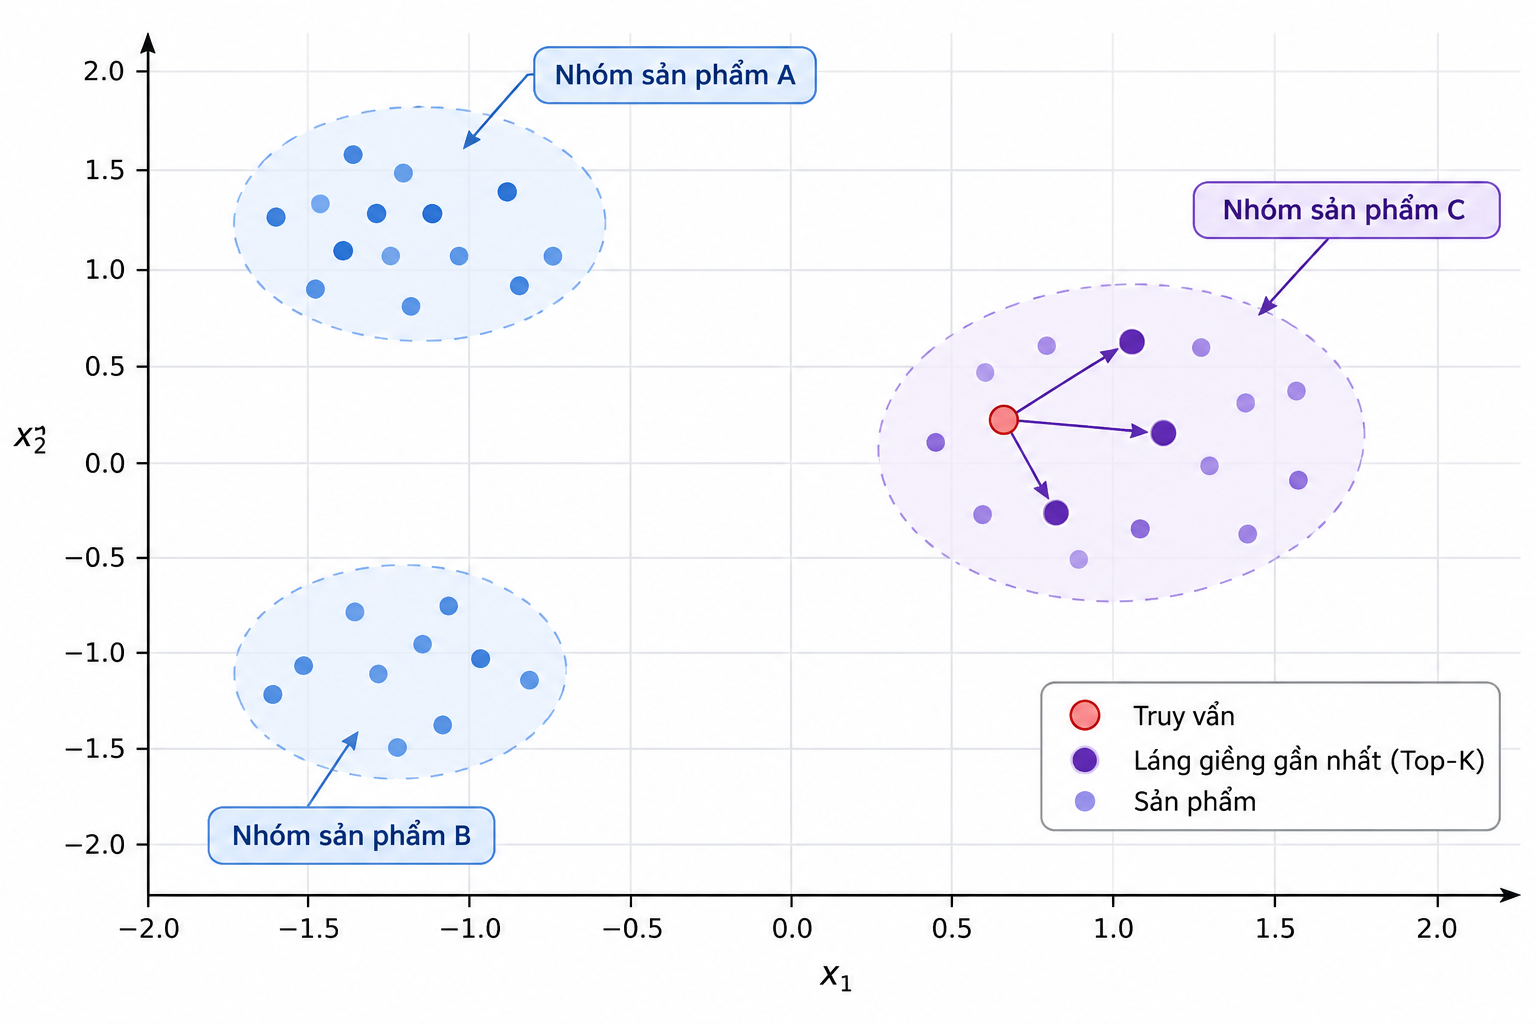
\includegraphics[width=0.85\textwidth]{Image/vector.png}
    \caption{Biểu diễn các đối tượng trong không gian vector}
    \label{fig:vector_space}
\end{figure}

\subsection{Text Embedding và Image Embedding}
\textbf{Text Embedding} là quá trình chuyển đổi văn bản thành vector biểu diễn ngữ nghĩa. Kỹ thuật này cho phép tìm kiếm các nội dung liên quan ngay cả khi không sử dụng từ khóa giống nhau. Trong hệ thống RAG, Text Embedding được sử dụng để biểu diễn truy vấn người dùng và thông tin sản phẩm.\\\\
\textbf{Image Embedding} là quá trình trích xuất đặc trưng hình ảnh và biểu diễn dưới dạng vector. Các vector này được sử dụng để so sánh mức độ tương đồng giữa hình ảnh đầu vào và hình ảnh sản phẩm, hỗ trợ chức năng tìm kiếm bằng hình ảnh.

\subsection{Độ tương đồng Cosine và chuẩn hóa L2}
Cosine Similarity là phương pháp đo mức độ tương đồng giữa hai vector dựa trên cosin của góc tạo bởi chúng, được xác định bằng công thức:
\[
\operatorname{sim}(A,B)=
\frac{\mathbf{A}\cdot\mathbf{B}}
{\|\mathbf{A}\|\|\mathbf{B}\|}
\]
Trong đó, $\mathbf{A}\cdot\mathbf{B}$ là tích vô hướng, còn $\|\mathbf{A}\|$ và $\|\mathbf{B}\|$ là độ dài của hai vector. Giá trị tương đồng nằm trong khoảng $[-1,1]$, với giá trị càng gần 1 thể hiện hướng của hai vector càng tương đồng.\\\\
Chuẩn hóa L2 đưa vector khác vector không về độ dài đơn vị mà không thay đổi hướng của nó:
\[
\hat{\mathbf{v}}=
\frac{\mathbf{v}}{\|\mathbf{v}\|_2},
\qquad
\|\mathbf{v}\|_2=
\sqrt{\sum_{i=1}^{d}v_i^2}
\]
Khi hai vector đã được chuẩn hóa L2, độ tương đồng Cosine có thể tính trực tiếp bằng tích vô hướng:
\[
\operatorname{sim}(A,B)=
\hat{\mathbf{A}}\cdot\hat{\mathbf{B}}
\]
Các phép toán trên được sử dụng trong tìm kiếm ngữ nghĩa và truy xuất những sản phẩm có đặc trưng tương đồng.

\subsection{Tìm kiếm láng giềng gần nhất và HNSW}
Tìm kiếm láng giềng gần nhất (Nearest Neighbor Search -- NNS) là phương pháp xác định các vector có khoảng cách nhỏ nhất hoặc độ tương đồng cao nhất với vector truy vấn.\\\\
Với tập vector $V$ và truy vấn $\mathbf{q}$, hệ thống tìm kiếm $K$ vector có mức độ tương đồng cao nhất để trả về kết quả Top-K.\\\\
Đối với tập dữ liệu lớn, việc so sánh toàn bộ vector có thể làm tăng thời gian xử lý. Vì vậy, các thuật toán tìm kiếm láng giềng gần đúng (Approximate Nearest Neighbor -- ANN) được sử dụng để tăng tốc độ truy xuất.\\\\
Hierarchical Navigable Small World (HNSW) là thuật toán ANN tổ chức các vector thành đồ thị nhiều tầng. Quá trình tìm kiếm bắt đầu từ tầng cao và di chuyển xuống các tầng thấp để xác định những vector gần với truy vấn.
\begin{figure}[H]
    \centering
    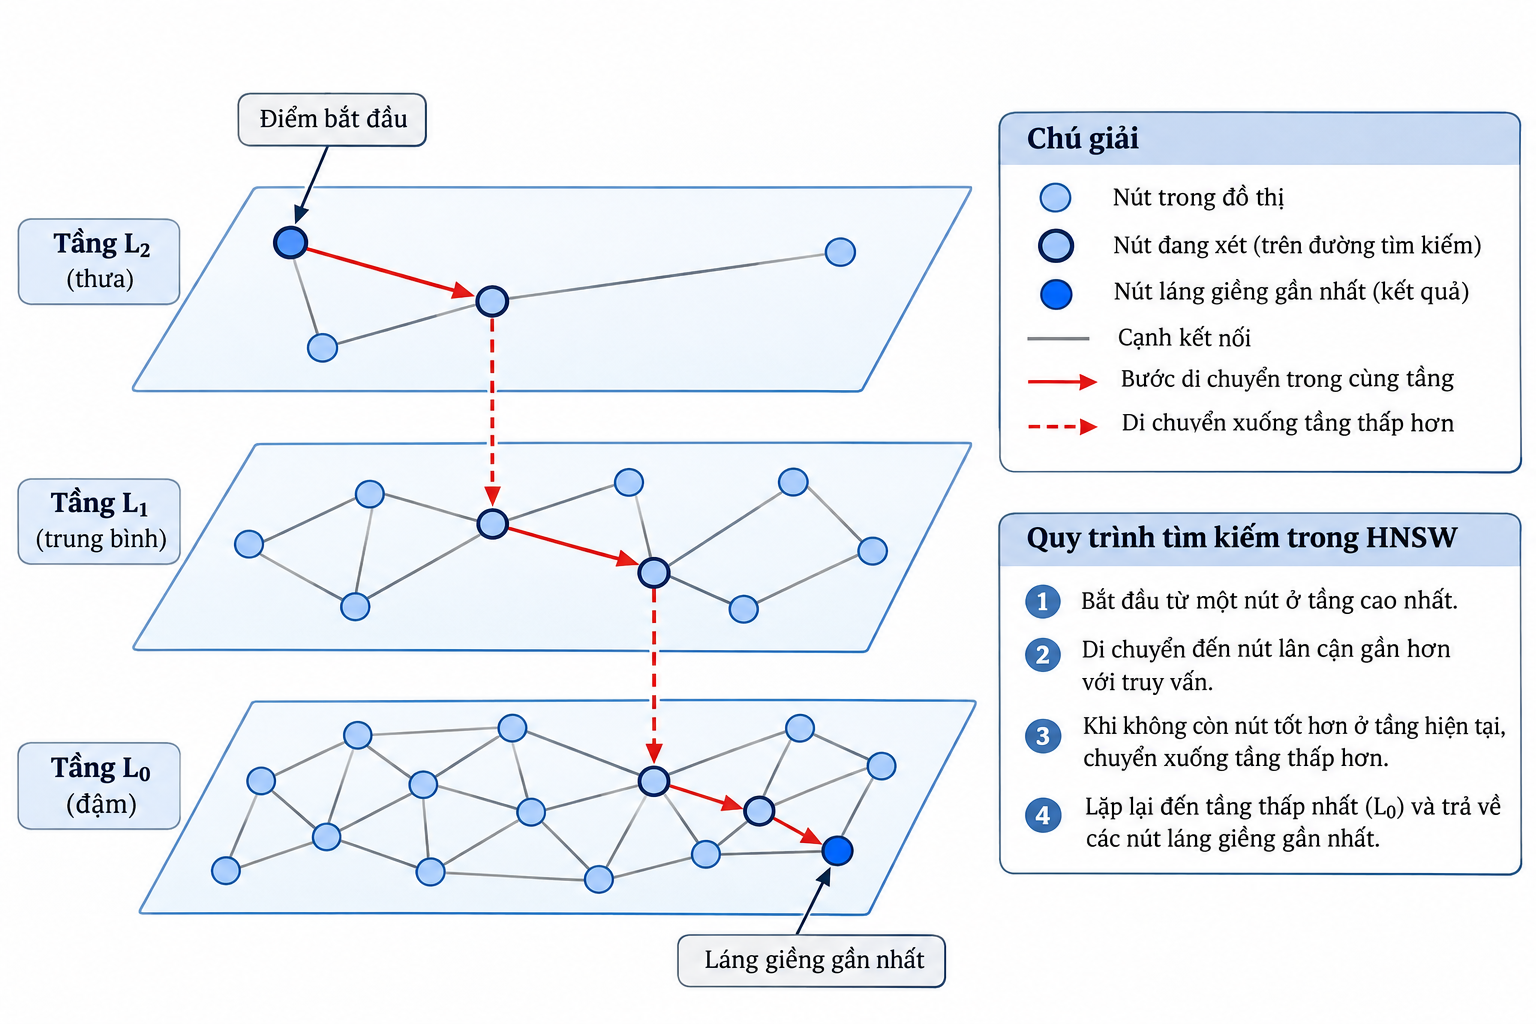
\includegraphics[width=0.95\textwidth]{Image/hnsw.png}
    \caption{Cấu trúc đồ thị nhiều tầng và quá trình tìm kiếm HNSW}
    \label{fig:hnsw}
\end{figure}
HNSW giúp tăng tốc độ tìm kiếm trên tập dữ liệu lớn, nhưng có thể đánh đổi một phần độ chính xác so với tìm kiếm chính xác.\\\\
Trong TechWiseAI, biểu diễn vector và tìm kiếm tương đồng là cơ sở kỹ thuật cho chatbot RAG, tìm kiếm sản phẩm bằng hình ảnh và hệ thống gợi ý sản phẩm.


\section{Mô hình ngôn ngữ lớn và kỹ thuật RAG}
\subsection{Mô hình ngôn ngữ lớn (LLM)}
Mô hình ngôn ngữ lớn (Large Language Model -- LLM) là mô hình học sâu được huấn luyện trên lượng lớn dữ liệu văn bản, có khả năng hiểu và sinh ngôn ngữ tự nhiên. Phần lớn LLM hiện đại sử dụng kiến trúc Transformer với cơ chế Attention để xử lý mối quan hệ giữa các thành phần trong ngữ cảnh.\\\\
LLM được ứng dụng trong các tác vụ như trả lời câu hỏi, tóm tắt và tư vấn. Tuy nhiên, mô hình có thể tạo ra thông tin không chính xác (Hallucination) và không tự động cập nhật dữ liệu của ứng dụng. Vì vậy, trong thương mại điện tử, LLM cần được kết hợp với cơ chế truy xuất thông tin để cung cấp nội dung tư vấn dựa trên dữ liệu sản phẩm.\\\\

\subsection{Kỹ thuật RAG và tiền xử lý dữ liệu}
Retrieval-Augmented Generation (RAG) là kỹ thuật kết hợp truy xuất thông tin (Retrieval) với mô hình ngôn ngữ lớn để sinh câu trả lời dựa trên dữ liệu bên ngoài.\\\\
Quy trình RAG gồm hai giai đoạn chính:
\begin{itemize}
    \item \textbf{Chuẩn bị dữ liệu:} Thu thập, làm sạch, chuẩn hóa và chuyển đổi dữ liệu thành vector embedding để phục vụ truy xuất.
    \item \textbf{Xử lý truy vấn:} Tiếp nhận câu hỏi, truy xuất thông tin liên quan và cung cấp ngữ cảnh cho LLM để sinh câu trả lời.
\end{itemize}
Quá trình sinh câu trả lời được biểu diễn khái quát như sau:
\[
A=\operatorname{LLM}(Q,C)
\]
Trong đó, $Q$ là câu hỏi, $C$ là ngữ cảnh được truy xuất và $A$ là câu trả lời được tạo ra.\\\\
Trong quá trình chuẩn bị dữ liệu, Chunking được sử dụng để chia tài liệu thành các đơn vị truy xuất phù hợp. Đối với dữ liệu sản phẩm có cấu trúc, mỗi sản phẩm có thể được biểu diễn thành một đơn vị dữ liệu riêng nếu đáp ứng giới hạn đầu vào của mô hình embedding.\\\\
Trong TechWiseAI, RAG cho phép chatbot khai thác thông tin sản phẩm từ cơ sở dữ liệu nhằm hỗ trợ tư vấn và hạn chế việc tạo ra thông tin thiếu căn cứ.
\begin{figure}[H]
    \centering
    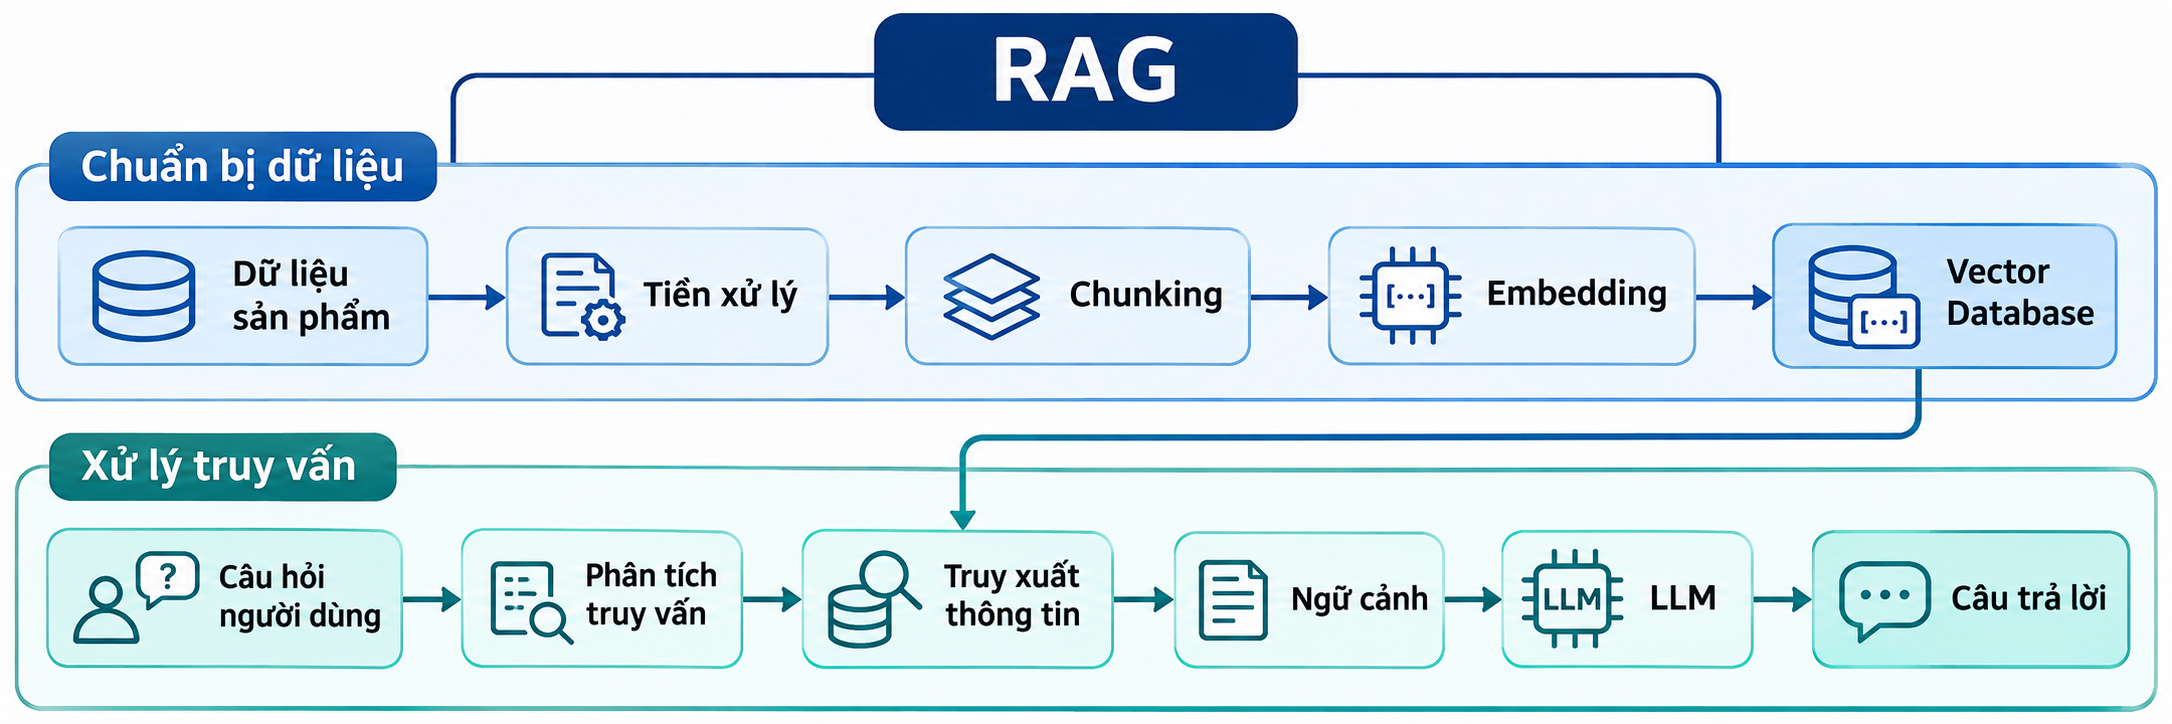
\includegraphics[width=\textwidth]{Image/rag.png}
    \caption{Quy trình hoạt động tổng quát của kỹ thuật RAG}
    \label{fig:rag_workflow}
\end{figure}

\subsection{Truy xuất thông tin và Hybrid Search}
Truy xuất thông tin (Retrieval) là quá trình tìm kiếm các tài liệu hoặc sản phẩm có mức độ liên quan cao với câu hỏi của người dùng.\\\\
Trước khi truy xuất, hệ thống có thể phân tích truy vấn để xác định các điều kiện như danh mục, thương hiệu, khoảng giá và nhu cầu sử dụng.\\\\
Hai phương pháp tìm kiếm phổ biến gồm:
\begin{itemize}
    \item \textbf{Keyword Search:} Tìm kiếm dựa trên từ khóa, phù hợp với tên sản phẩm, thương hiệu và thông số cụ thể.
    \item \textbf{Semantic Search:} Sử dụng vector embedding để tìm kiếm dựa trên mức độ tương đồng ngữ nghĩa.
\end{itemize}
Hybrid Search kết hợp hai phương pháp trên nhằm tận dụng ưu điểm của từng kỹ thuật. Kết quả truy xuất có thể được tổng hợp bằng thuật toán Reciprocal Rank Fusion (RRF):
\[
\operatorname{RRF}(d)=
\sum_{i=1}^{m}
\frac{1}{k+r_i(d)}
\]
Trong đó, $m$ là số danh sách kết quả, $k$ là hằng số điều chỉnh và $r_i(d)$ là thứ hạng của tài liệu $d$ trong danh sách thứ $i$. Các danh sách không chứa tài liệu $d$ không đóng góp vào tổng điểm.\\\\
RRF kết hợp kết quả dựa trên thứ hạng mà không yêu cầu chuẩn hóa điểm số, giúp lựa chọn các sản phẩm liên quan từ nhiều phương pháp tìm kiếm.
\begin{figure}[H]
    \centering
    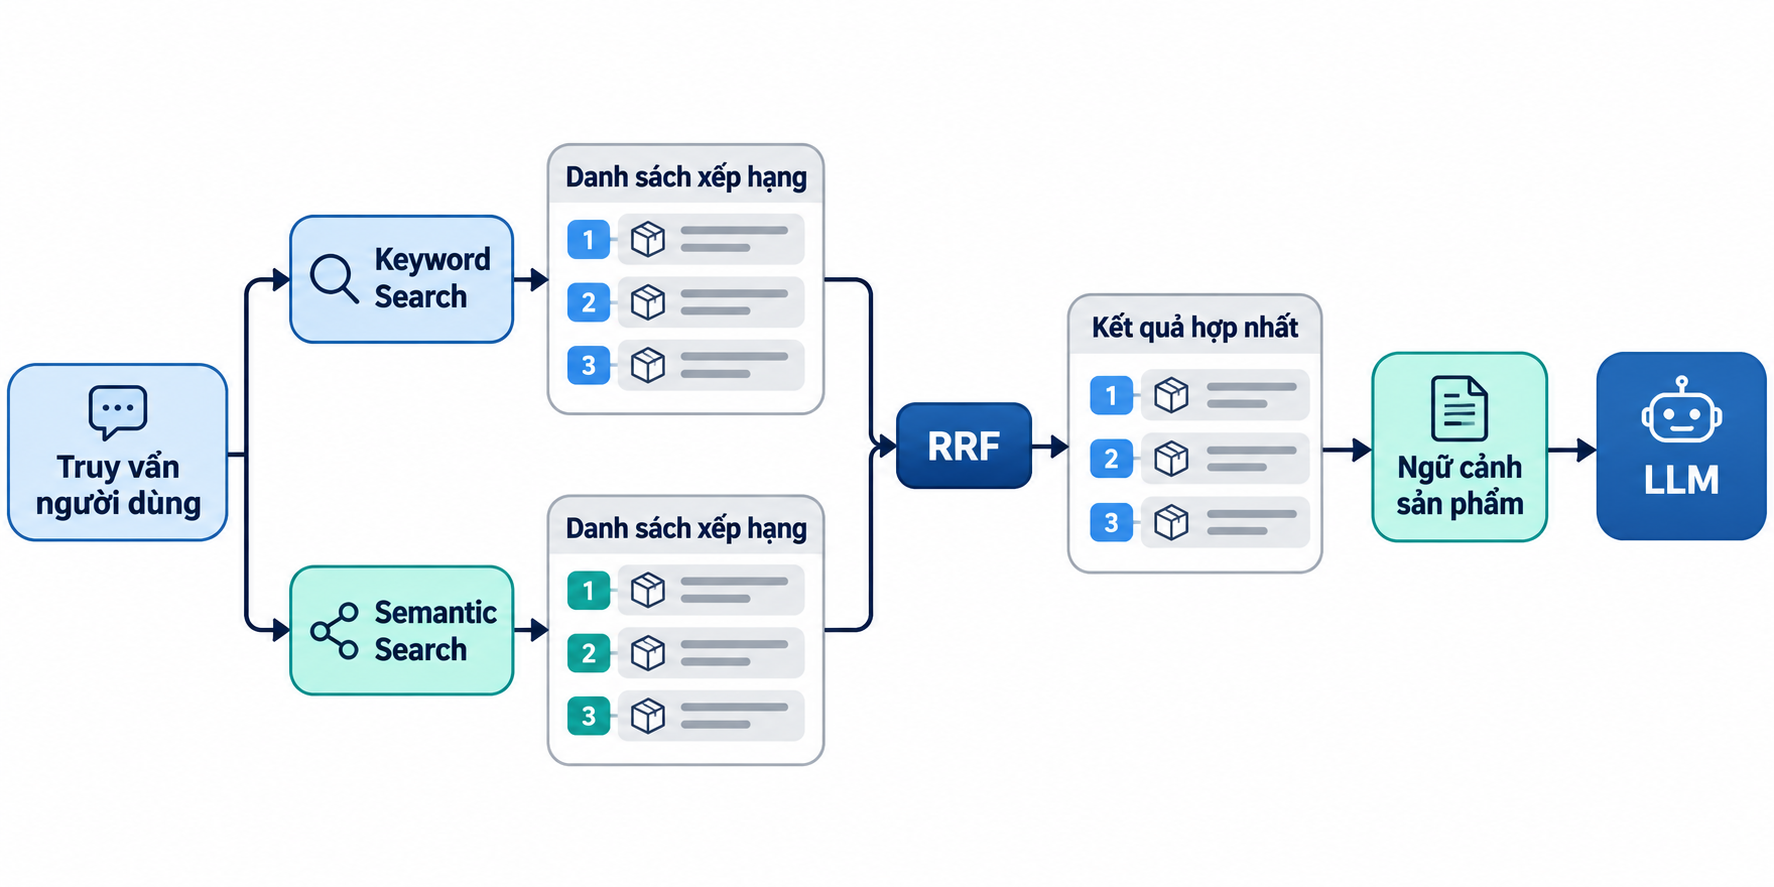
\includegraphics[width=\textwidth]{Image/hybrid.png}
    \caption{Quy trình Hybrid Search kết hợp thuật toán RRF}
    \label{fig:hybrid_search}
\end{figure}

\subsection{Reranking và sinh câu trả lời}
Reranking là bước đánh giá và sắp xếp lại các kết quả truy xuất nhằm lựa chọn những tài liệu phù hợp nhất với câu hỏi. Bước này có thể sử dụng mô hình Cross-Encoder để đánh giá mức độ liên quan giữa truy vấn và từng tài liệu.\\\\
Reranking là bước tùy chọn vì có thể làm tăng thời gian xử lý và chi phí tính toán.\\\\
Sau khi truy xuất, hệ thống kết hợp câu hỏi với thông tin sản phẩm liên quan để xây dựng Prompt cho LLM. Mô hình sử dụng ngữ cảnh được cung cấp để tạo câu trả lời, đồng thời cần tránh đưa ra giá bán hoặc thông số kỹ thuật không có trong dữ liệu.\\\\
Trong chatbot RAG, cơ chế Streaming có thể được sử dụng để truyền nội dung phản hồi từng phần, giúp người dùng theo dõi câu trả lời ngay trong quá trình sinh văn bản.


\section{Thị giác máy tính và tìm kiếm hình ảnh}
\subsection{Tìm kiếm hình ảnh dựa trên nội dung (CBIR)}
Tìm kiếm hình ảnh dựa trên nội dung (Content-Based Image Retrieval -- CBIR) là phương pháp truy xuất hình ảnh dựa trên các đặc trưng trực quan như màu sắc, hình dạng, kết cấu và ngữ nghĩa thay vì chỉ sử dụng từ khóa hoặc thông tin mô tả.\\\\
Với sự phát triển của học sâu, các mô hình có thể tự động trích xuất đặc trưng hình ảnh và biểu diễn chúng dưới dạng vector. Quá trình tìm kiếm được thực hiện bằng cách so sánh vector của hình ảnh truy vấn với các vector đã lưu trữ, sau đó trả về những sản phẩm có mức độ tương đồng cao nhất.\\\\
Trong thương mại điện tử, CBIR giúp người dùng tìm kiếm sản phẩm bằng hình ảnh mà không cần biết chính xác tên gọi hoặc mã sản phẩm.

\subsection{Mô hình SigLIP}
Sigmoid Loss for Language Image Pre-training (SigLIP) là phương pháp tiền huấn luyện mô hình kết hợp hình ảnh và văn bản nhằm học mối quan hệ ngữ nghĩa giữa hai loại dữ liệu.\\\\
SigLIP sử dụng kiến trúc Dual-Encoder gồm bộ mã hóa hình ảnh (Image Encoder) và bộ mã hóa văn bản (Text Encoder). Hai bộ mã hóa chuyển đổi dữ liệu đầu vào thành các vector đặc trưng có thể so sánh trong cùng không gian biểu diễn.\\\\
Điểm nổi bật của SigLIP là sử dụng hàm mất mát Sigmoid để học mối quan hệ giữa các cặp hình ảnh và văn bản. Nhờ đó, bộ mã hóa hình ảnh có thể được sử dụng để trích xuất đặc trưng phục vụ tìm kiếm hình ảnh tương đồng.
\begin{figure}[H]
    \centering
    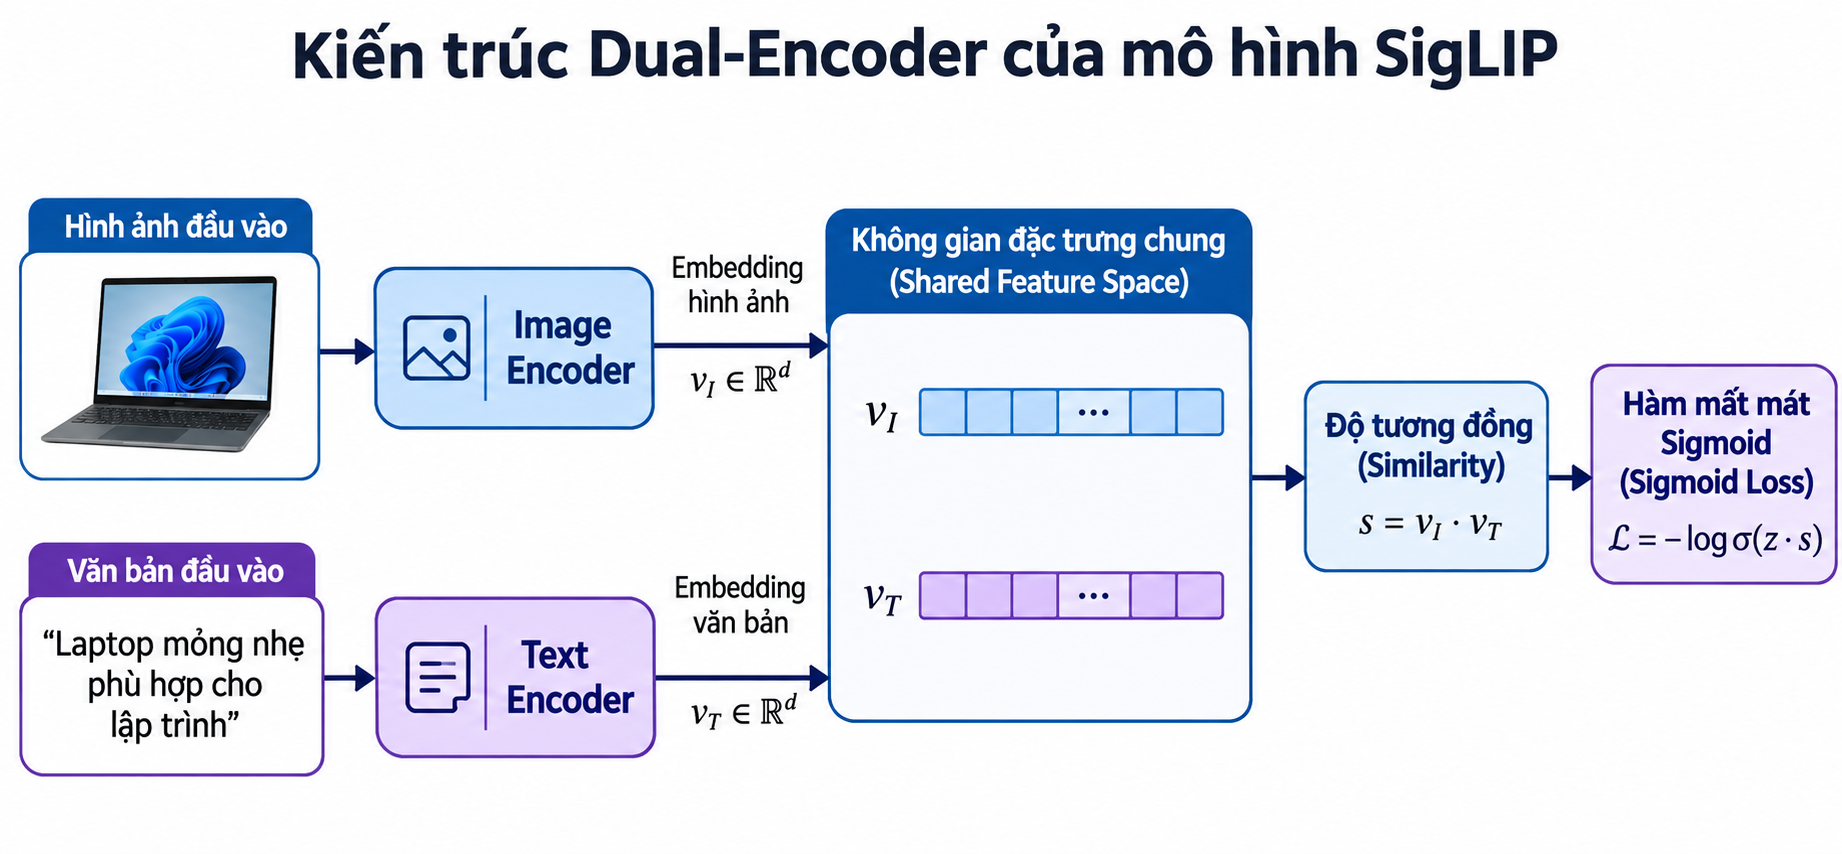
\includegraphics[width=0.95\textwidth]{Image/siglip.png}
    \caption{Kiến trúc Dual-Encoder của mô hình SigLIP}
    \label{fig:siglip}
\end{figure}

\subsection{Trích xuất đặc trưng và truy xuất hình ảnh tương đồng}
Trích xuất đặc trưng hình ảnh là quá trình sử dụng mô hình học sâu để chuyển đổi hình ảnh thành vector biểu diễn. Với hình ảnh đầu vào $I$, quá trình này được mô tả như sau:
\[
\mathbf{v}_I=f_{\theta}(I)
\]
Trong đó, $f_{\theta}$ là mô hình trích xuất đặc trưng và $\mathbf{v}_I$ là vector biểu diễn hình ảnh.\\\\
Trong hệ thống tìm kiếm sản phẩm, các hình ảnh được tiền xử lý và chuyển đổi thành vector để lưu trữ. Khi người dùng tải lên hình ảnh mới, hệ thống trích xuất vector truy vấn và so sánh với các vector đã lưu bằng độ tương đồng Cosine.\\\\
Những sản phẩm có mức độ tương đồng cao nhất được lựa chọn theo phương pháp Top-K và trả về cho người dùng. Kết quả thể hiện mức độ tương đồng theo đặc trưng hình ảnh, không nhất thiết là cùng một sản phẩm.
\begin{figure}[H]
    \centering
    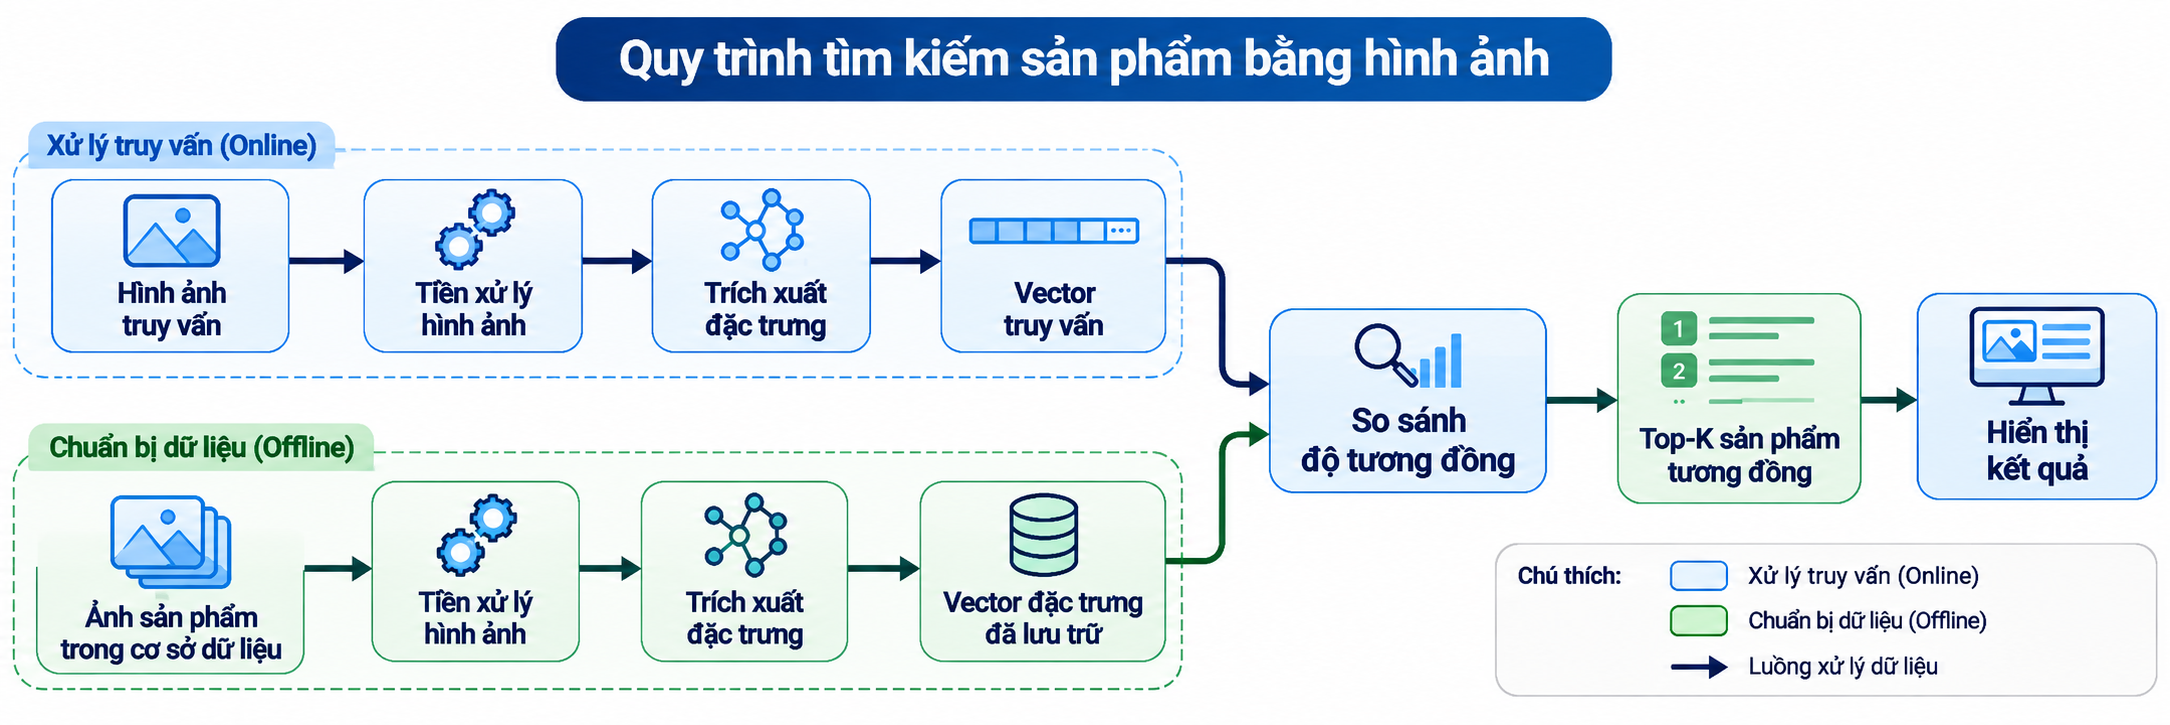
\includegraphics[width=\textwidth]{Image/image_search.png}
    \caption{Quy trình tìm kiếm sản phẩm bằng hình ảnh}
    \label{fig:image_search_workflow}
\end{figure}


\section{Hệ thống gợi ý và cá nhân hóa sản phẩm}
\subsection{Tổng quan về hệ thống gợi ý}
Hệ thống gợi ý (Recommender System) là hệ thống phân tích dữ liệu nhằm dự đoán sở thích và đề xuất những sản phẩm phù hợp với người dùng.\\\\
Các phương pháp gợi ý phổ biến bao gồm:
\begin{itemize}
    \item \textbf{Content-Based Recommendation:} Gợi ý dựa trên đặc trưng sản phẩm và sở thích người dùng.
    \item \textbf{Behavior-Based Recommendation:} Gợi ý dựa trên lịch sử tương tác của người dùng.
    \item \textbf{Hybrid Recommendation:} Kết hợp nhiều phương pháp nhằm nâng cao chất lượng đề xuất.
\end{itemize}
Trong thương mại điện tử, việc kết hợp đặc trưng sản phẩm và dữ liệu hành vi giúp hệ thống cá nhân hóa danh sách sản phẩm theo nhu cầu của từng người dùng.

\subsection{Phân tích hành vi và xây dựng hồ sơ sở thích}
Hành vi người dùng là nguồn dữ liệu phản ánh mức độ quan tâm đối với sản phẩm, bao gồm xem, nhấp vào, yêu thích, thêm vào giỏ hàng và mua hàng. Các tương tác này được xem là phản hồi ngầm (Implicit Feedback) và có thể được gán trọng số khác nhau.\\\\
Thông tin sản phẩm được biểu diễn thành vector thông qua các mô hình mã hóa văn bản như Sentence Transformers. Hồ sơ sở thích người dùng (User Preference Profile) có thể được xây dựng bằng cách tổng hợp các vector sản phẩm đã tương tác theo trọng số:
\[
\mathbf{p}_u =
\frac{\sum_{i=1}^{n} w_i\mathbf{v}_i}
{\sum_{i=1}^{n} w_i}
\]
Trong đó, $\mathbf{p}_u$ là vector sở thích người dùng, $\mathbf{v}_i$ là vector sản phẩm và $w_i$ là trọng số tương tác, với tổng trọng số khác 0.\\\\
Để phản ánh sự thay đổi sở thích theo thời gian, hệ thống có thể áp dụng kỹ thuật Time Decay nhằm giảm ảnh hưởng của những tương tác cũ. Ngoài vector sở thích, hồ sơ người dùng còn có thể lưu thông tin về danh mục, thương hiệu và khoảng giá thường quan tâm.
\begin{figure}[H]
    \centering
    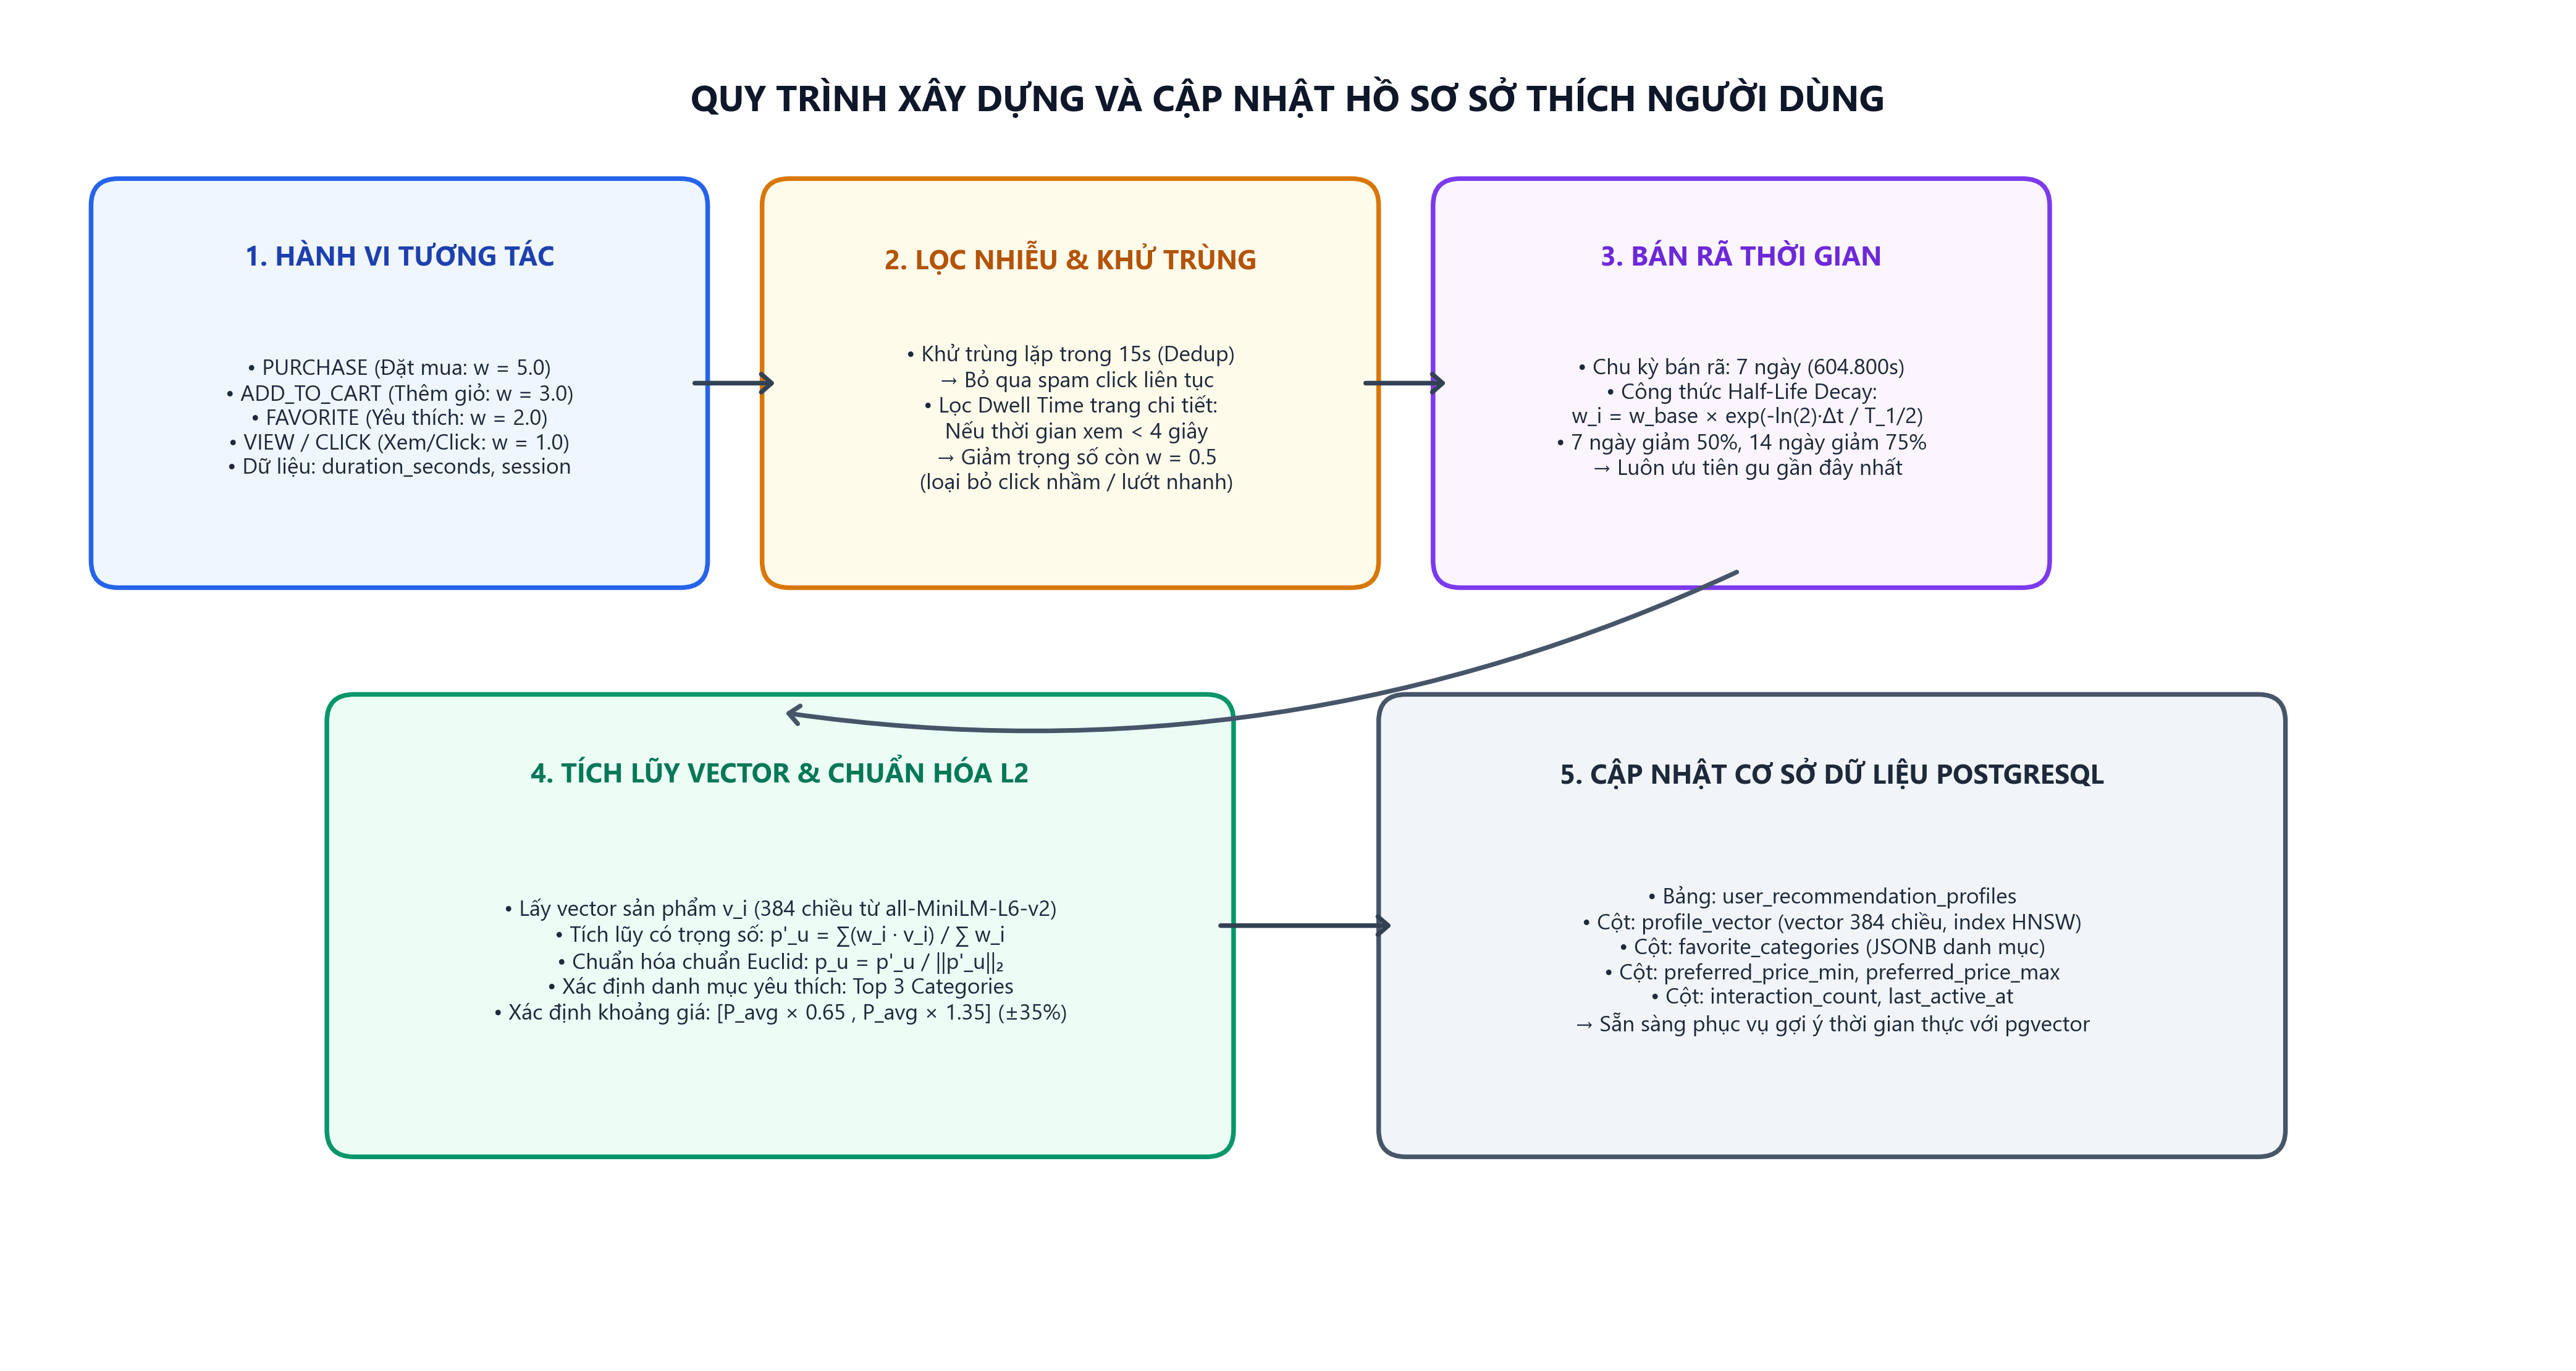
\includegraphics[width=\textwidth]{Image/user_profile.png}
    \caption{Quy trình xây dựng hồ sơ sở thích người dùng}
    \label{fig:user_profile}
\end{figure}

\subsection{Xếp hạng sản phẩm đa tiêu chí}
Xếp hạng đa tiêu chí (Multi-Factor Ranking) là phương pháp đánh giá mức độ phù hợp của sản phẩm dựa trên nhiều yếu tố, bao gồm độ tương đồng ngữ nghĩa, danh mục, thương hiệu và khoảng giá.\\\\
Điểm phù hợp của sản phẩm $i$ đối với người dùng $u$ có thể được xác định như sau:
\[
S(u,i)=
\alpha S_{\text{semantic}}+
\beta S_{\text{category}}+
\gamma S_{\text{brand}}+
\delta S_{\text{price}}
\]
Trong đó, các thành phần $S$ biểu diễn điểm phù hợp theo từng tiêu chí; $\alpha$, $\beta$, $\gamma$, $\delta$ là các trọng số điều chỉnh, thường được lựa chọn sao cho tổng bằng 1.\\\\
Các điểm thành phần cần được đưa về thang đo phù hợp trước khi kết hợp. Sau khi tính điểm, hệ thống sắp xếp sản phẩm theo thứ tự giảm dần và lựa chọn những sản phẩm có điểm cao nhất để đề xuất.
\begin{figure}[H]
    \centering
    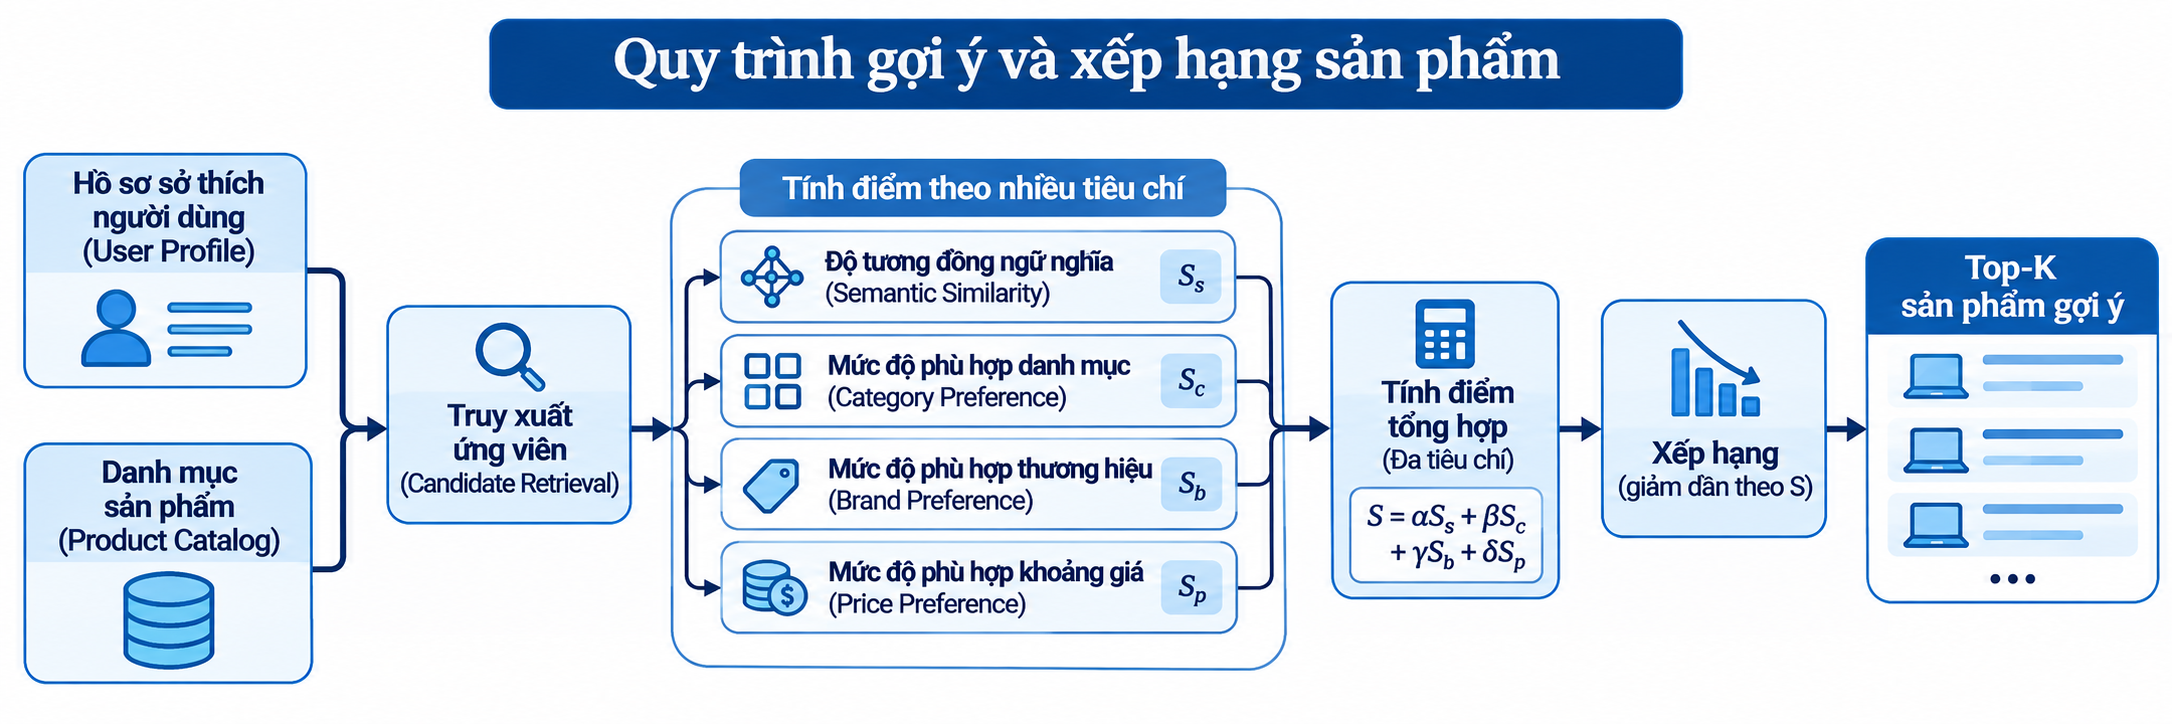
\includegraphics[width=\textwidth]{Image/rr.png}
    \caption{Quy trình gợi ý và xếp hạng sản phẩm đa tiêu chí}
    \label{fig:recommendation_ranking}
\end{figure}

\subsection{Bài toán Cold Start}
Cold Start xảy ra khi hệ thống chưa có đủ dữ liệu tương tác để xác định sở thích của người dùng mới hoặc thiếu thông tin về sản phẩm mới.\\\\
Để giải quyết vấn đề này, hệ thống có thể ưu tiên gợi ý các sản phẩm phổ biến, nổi bật hoặc mới được cập nhật. Khi người dùng phát sinh thêm tương tác, hồ sơ sở thích được cập nhật để từng bước chuyển sang gợi ý cá nhân hóa.\\\\
Trong TechWiseAI, các phương pháp phân tích hành vi, biểu diễn vector và xếp hạng đa tiêu chí là cơ sở để xây dựng chức năng đề xuất sản phẩm phù hợp với sở thích người dùng.

\chapter{PHÂN TÍCH VÀ THIẾT KẾ HỆ THỐNG}
\section{Phân tích yêu cầu hệ thống}
\subsection{Mô tả bài toán}
Việc lựa chọn sản phẩm công nghệ thường gặp khó khăn do sự đa dạng về thương hiệu, thông số kỹ thuật và mức giá. Các phương pháp tìm kiếm truyền thống dựa trên từ khóa và bộ lọc chưa đáp ứng đầy đủ nhu cầu tìm kiếm bằng ngôn ngữ tự nhiên, hình ảnh và cá nhân hóa sản phẩm.\\\\
Xuất phát từ thực tế trên, TechWiseAI được xây dựng như một website thương mại điện tử kinh doanh sản phẩm công nghệ, cung cấp các chức năng quản lý tài khoản, tìm kiếm sản phẩm, giỏ hàng, đặt hàng, thanh toán và quản trị hệ thống.\\\\
Bên cạnh đó, hệ thống tích hợp ba chức năng trí tuệ nhân tạo gồm chatbot tư vấn ứng dụng RAG, tìm kiếm sản phẩm bằng hình ảnh và gợi ý sản phẩm theo hành vi người dùng. Các chức năng này nhằm hỗ trợ quá trình tìm kiếm, lựa chọn và mua sắm sản phẩm phù hợp với nhu cầu.

\subsection{Xác định các tác nhân của hệ thống}
Hệ thống TechWiseAI bao gồm các tác nhân chính:
\begin{itemize}
    \item \textbf{Khách truy cập (Guest):} Xem, tìm kiếm sản phẩm, đọc tin tức, sử dụng chatbot và tìm kiếm bằng hình ảnh mà không cần đăng nhập.
    \item \textbf{Khách hàng (Customer):} Sử dụng các chức năng công khai, đồng thời quản lý tài khoản, giỏ hàng, danh sách yêu thích, đặt hàng, thanh toán, theo dõi đơn hàng và đánh giá sản phẩm.
    \item \textbf{Quản trị viên (Administrator):} Quản lý sản phẩm, danh mục, người dùng, đơn hàng, đánh giá, bài viết và theo dõi thống kê kho hàng.
    \item \textbf{VNPay Sandbox:} Hệ thống bên ngoài hỗ trợ xử lý và xác nhận kết quả thanh toán trực tuyến trong môi trường thử nghiệm.
\end{itemize}

\subsection{Yêu cầu chức năng}
Các yêu cầu chức năng của TechWiseAI được chia thành những nhóm chính:
\begin{itemize}
    \item \textbf{Quản lý tài khoản:} Đăng ký, đăng nhập, cập nhật thông tin cá nhân và phân quyền người dùng.
    \item \textbf{Quản lý sản phẩm:} Hiển thị, tìm kiếm, lọc, so sánh sản phẩm và quản lý danh sách yêu thích; hỗ trợ quản trị viên cập nhật sản phẩm, hình ảnh và danh mục.
    \item \textbf{Giỏ hàng và đơn hàng:} Thêm, sửa, xóa sản phẩm trong giỏ hàng; đặt hàng, theo dõi, hủy đơn hàng theo điều kiện và quản lý trạng thái đơn hàng.
    \item \textbf{Thanh toán trực tuyến:} Tích hợp VNPay Sandbox, tiếp nhận và xác minh kết quả giao dịch để cập nhật trạng thái thanh toán.
    \item \textbf{Quản lý nội dung:} Hiển thị bài viết, đánh giá sản phẩm; hỗ trợ quản trị viên quản lý bài viết và kiểm duyệt đánh giá.
    \item \textbf{Quản trị và thống kê:} Quản lý người dùng, sản phẩm, đơn hàng và theo dõi tình trạng kho hàng.
    \item \textbf{Chatbot RAG:} Tiếp nhận câu hỏi bằng ngôn ngữ tự nhiên, truy xuất dữ liệu sản phẩm và sinh câu trả lời tư vấn, hỗ trợ liên kết sản phẩm và phản hồi theo luồng (Streaming).
    \item \textbf{Tìm kiếm bằng hình ảnh:} Tiếp nhận hình ảnh đầu vào, tìm kiếm và hiển thị các sản phẩm có đặc điểm tương đồng.
    \item \textbf{Gợi ý sản phẩm:} Đề xuất sản phẩm tương tự và cá nhân hóa danh sách gợi ý dựa trên lịch sử tương tác, có phương án thay thế khi chưa đủ dữ liệu hành vi.
\end{itemize}

\subsection{Yêu cầu phi chức năng}
Bên cạnh các chức năng nghiệp vụ, hệ thống cần đáp ứng những yêu cầu phi chức năng sau:
\begin{itemize}
    \item \textbf{Hiệu năng:} Bảo đảm thời gian phản hồi phù hợp, tối ưu truy xuất dữ liệu và hỗ trợ Streaming cho chatbot.
    \item \textbf{Bảo mật:} Xác thực, phân quyền truy cập, bảo vệ dữ liệu nhạy cảm và xác minh kết quả thanh toán.
    \item \textbf{Độ tin cậy:} Xử lý lỗi phù hợp, bảo đảm tính nhất quán của dữ liệu và hạn chế chatbot cung cấp thông tin không có căn cứ.
    \item \textbf{Khả năng mở rộng và bảo trì:} Phân tách các thành phần hệ thống để thuận tiện nâng cấp, kiểm thử và tích hợp chức năng mới.
    \item \textbf{Tính dễ sử dụng:} Giao diện trực quan, tương thích với nhiều kích thước màn hình và hỗ trợ thao tác mua sắm thuận tiện.
    \item \textbf{Tính nhất quán dữ liệu:} Bảo đảm thông tin sản phẩm được sử dụng trong các chức năng AI phù hợp với dữ liệu hiện có trên website.
    \item \textbf{Khả năng kiểm thử:} Hỗ trợ kiểm tra chức năng, đánh giá chất lượng kết quả AI và thời gian phản hồi của hệ thống.
\end{itemize}


\section{Phân tích chức năng hệ thống}

\subsection{Sơ đồ phân rã chức năng hệ thống}

Sơ đồ phân rã chức năng (Functional Decomposition Diagram -- FDD) thể hiện cấu trúc phân cấp các chức năng của TechWiseAI, làm cơ sở cho việc phân tích và xây dựng các sơ đồ Use Case.

Hệ thống được chia thành bảy nhóm chức năng chính: xác thực và tài khoản, sản phẩm và tìm kiếm, dịch vụ trí tuệ nhân tạo, tương tác sản phẩm, giỏ hàng và thanh toán, tin tức và bài viết, quản trị hệ thống.

\begin{figure}[H]
    \centering
    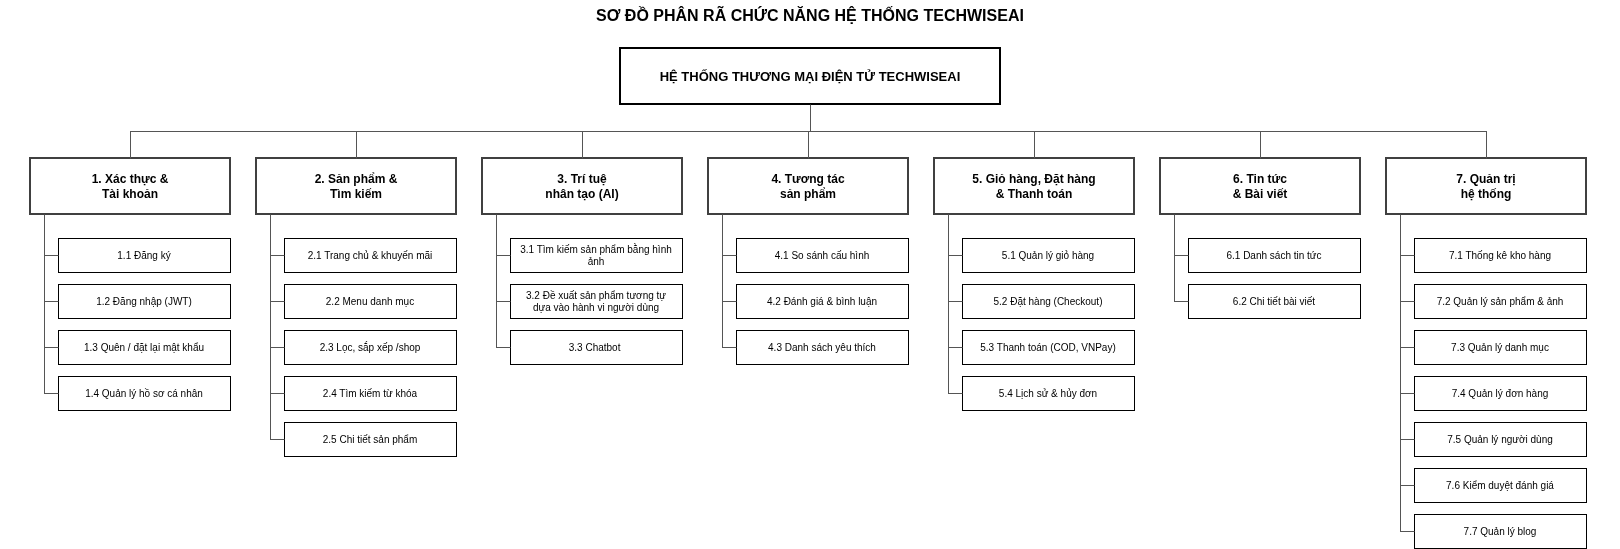
\includegraphics[width=\textwidth]{Image/FDD_Tong_quan.drawio.png}
    \caption{Sơ đồ phân rã chức năng hệ thống TechWiseAI}
    \label{fig:fdd-tong-quan}
\end{figure}

\subsection{Sơ đồ Use Case tổng quát}

Sơ đồ Use Case tổng quát mô tả mối quan hệ giữa các tác nhân và những chức năng chính của hệ thống.

TechWiseAI gồm ba tác nhân người dùng: khách truy cập (Guest), khách hàng (Customer) và quản trị viên (Administrator). Khách truy cập sử dụng các chức năng công khai; khách hàng được bổ sung các chức năng mua sắm và quản lý tài khoản; quản trị viên thực hiện các nghiệp vụ quản lý hệ thống. Ngoài ra, VNPay Sandbox tham gia vào quá trình thanh toán trực tuyến.

\begin{figure}[H]
    \centering
    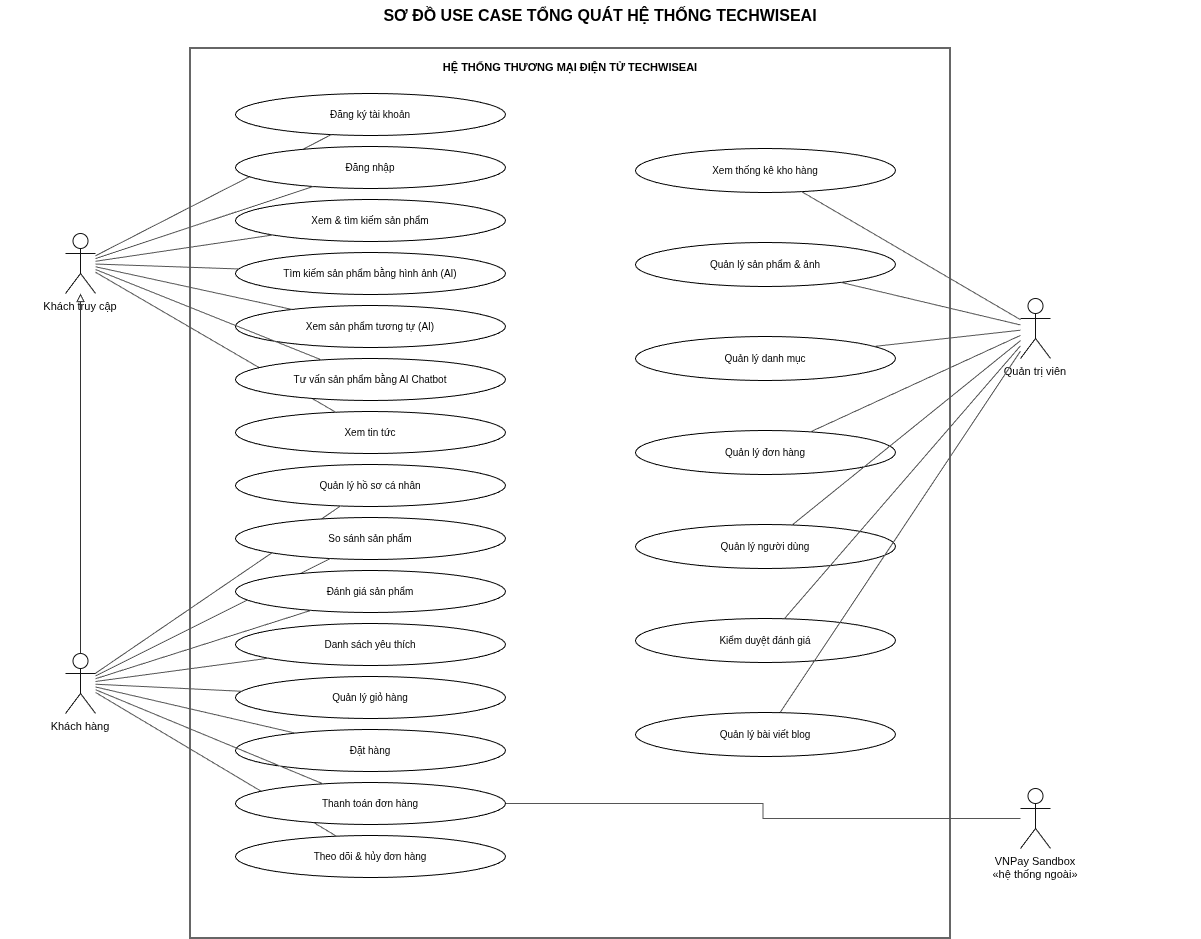
\includegraphics[width=\textwidth]{Image/UC-00_Use_Case_Tong_Quat_Chinh_Sua.drawio.png}
    \caption{Sơ đồ Use Case tổng quát hệ thống TechWiseAI}
    \label{fig:uc-tong-quat}
\end{figure}

\subsection{Phân tích chức năng xác thực và quản lý tài khoản}

Nhóm chức năng này hỗ trợ đăng ký, đăng nhập, khôi phục mật khẩu và quản lý hồ sơ cá nhân.

Hệ thống thực hiện kiểm tra thông tin đăng ký, xác thực người dùng bằng JWT và phân quyền truy cập. Khách hàng có thể cập nhật thông tin cá nhân, trong đó hình ảnh hồ sơ có thể được lưu trữ thông qua Cloudinary.

\begin{figure}[H]
    \centering
    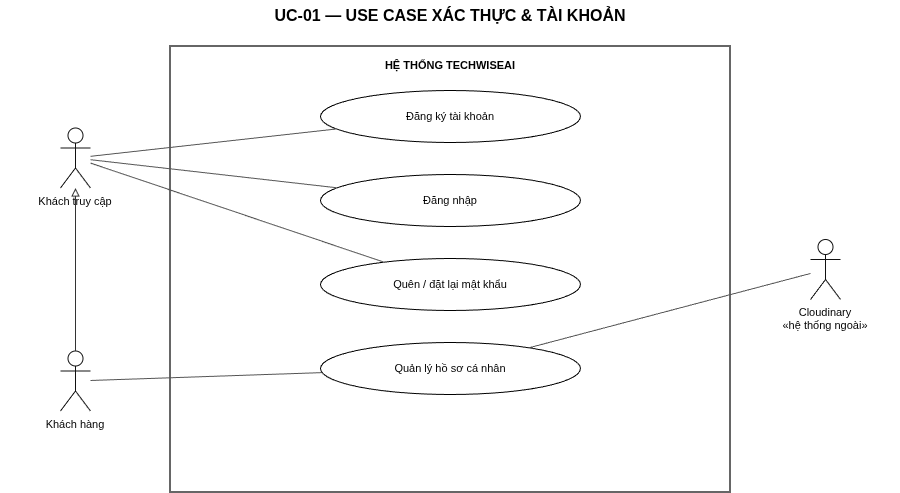
\includegraphics[width=\textwidth]{Image/UC-01_Xac_thuc_Tai_khoan.drawio.png}
    \caption{Sơ đồ Use Case xác thực và quản lý tài khoản}
    \label{fig:uc-xac-thuc}
\end{figure}

\subsection{Phân tích chức năng duyệt và khám phá sản phẩm}

Nhóm chức năng này cho phép người dùng xem trang chủ, chương trình ưu đãi, điều hướng danh mục, lọc, sắp xếp và xem thông tin sản phẩm.

Người dùng có thể tìm kiếm sản phẩm thuộc các danh mục như laptop, điện thoại, tai nghe, máy ảnh, linh kiện và phụ kiện. Hệ thống cung cấp thông tin chi tiết về giá bán, hình ảnh, mô tả và thông số kỹ thuật để hỗ trợ quá trình lựa chọn.

\begin{figure}[H]
    \centering
    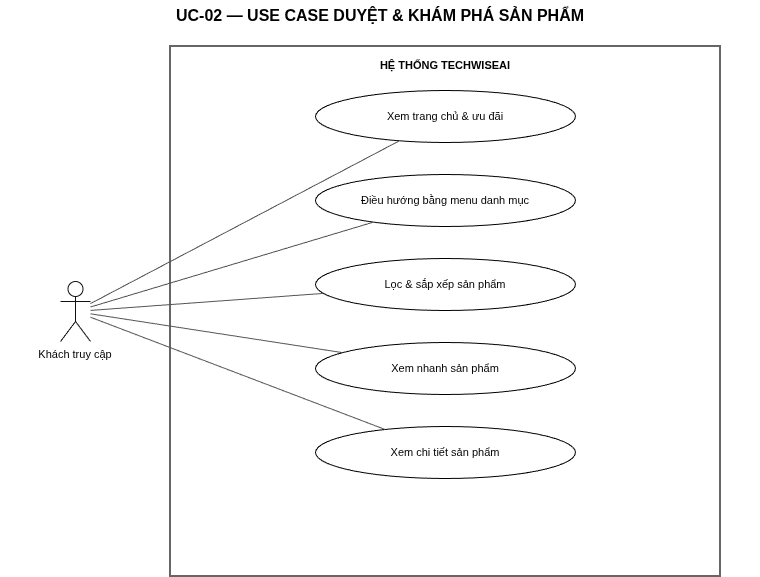
\includegraphics[width=\textwidth]{Image/UC-02_Duyet_Kham_pha_SP.drawio.png}
    \caption{Sơ đồ Use Case duyệt và khám phá sản phẩm}
    \label{fig:uc-kham-pha}
\end{figure}

\subsection{Phân tích chức năng dịch vụ trí tuệ nhân tạo}

Nhóm chức năng AI gồm ba chức năng chính:

\begin{itemize}
    \item \textbf{Tìm kiếm bằng hình ảnh:} Sử dụng mô hình SigLIP để trích xuất đặc trưng hình ảnh và truy xuất các sản phẩm tương đồng.

    \item \textbf{Gợi ý sản phẩm:} Đề xuất sản phẩm tương tự hoặc cá nhân hóa dựa trên đặc trưng sản phẩm và lịch sử tương tác của người dùng.

    \item \textbf{Chatbot tư vấn:} Ứng dụng RAG để truy xuất thông tin sản phẩm và sử dụng mô hình ngôn ngữ tạo câu trả lời phù hợp với nhu cầu.
\end{itemize}

Ngoài ra, hệ thống thực hiện tạo và cập nhật vector embedding để phục vụ các chức năng truy xuất dữ liệu AI.

\begin{figure}[H]
    \centering
    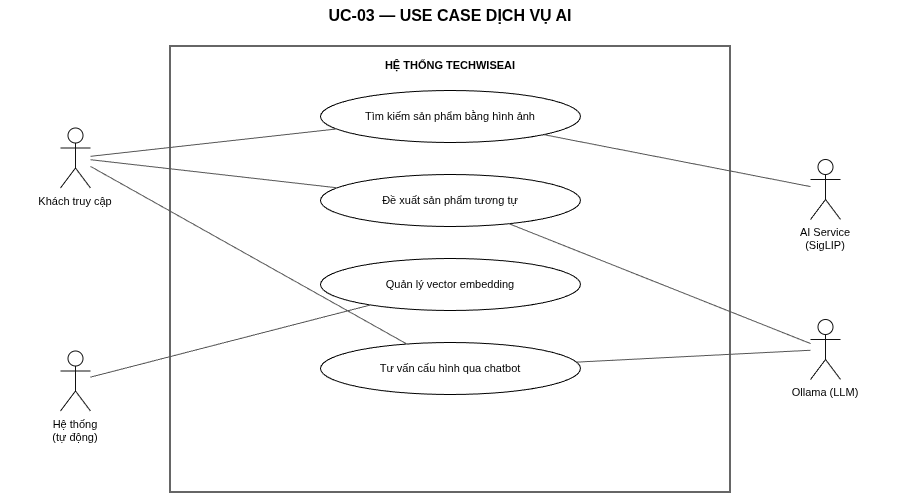
\includegraphics[width=\textwidth]{Image/UC-03_Dich_vu_AI.drawio.png}
    \caption{Sơ đồ Use Case dịch vụ trí tuệ nhân tạo}
    \label{fig:uc-ai}
\end{figure}

\subsection{Phân tích chức năng tương tác và so sánh sản phẩm}

Nhóm chức năng này hỗ trợ tìm kiếm bằng từ khóa, so sánh sản phẩm, đánh giá và quản lý danh sách yêu thích.

Người dùng có thể so sánh giá bán và thông số kỹ thuật giữa các sản phẩm. Khách hàng đã đăng nhập được phép đánh giá và lưu sản phẩm yêu thích. Dữ liệu tương tác cũng có thể được sử dụng để hỗ trợ hệ thống gợi ý cá nhân hóa.

\begin{figure}[H]
    \centering
    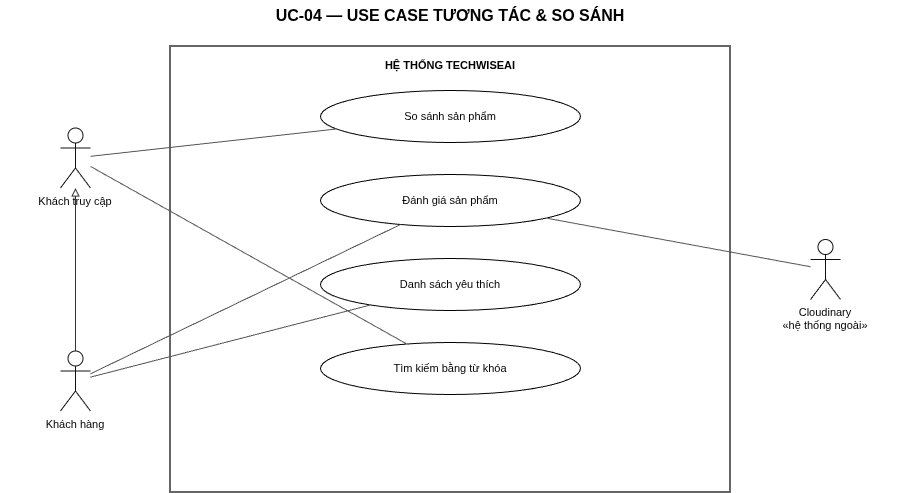
\includegraphics[width=\textwidth]{Image/UC-04_Tuong_tac_So_sanh.drawio.png}
    \caption{Sơ đồ Use Case tương tác và so sánh sản phẩm}
    \label{fig:uc-tuong-tac}
\end{figure}

\subsection{Phân tích chức năng giỏ hàng và thanh toán}

Nhóm chức năng này cho phép khách hàng quản lý giỏ hàng, đặt hàng, thanh toán, xem lịch sử và hủy đơn hàng theo điều kiện cho phép.

Hệ thống hỗ trợ thanh toán khi nhận hàng (COD) và thanh toán trực tuyến qua VNPay Sandbox. Đối với VNPay, kết quả giao dịch cần được xác minh trước khi cập nhật trạng thái thanh toán và đơn hàng.

\begin{figure}[H]
    \centering
    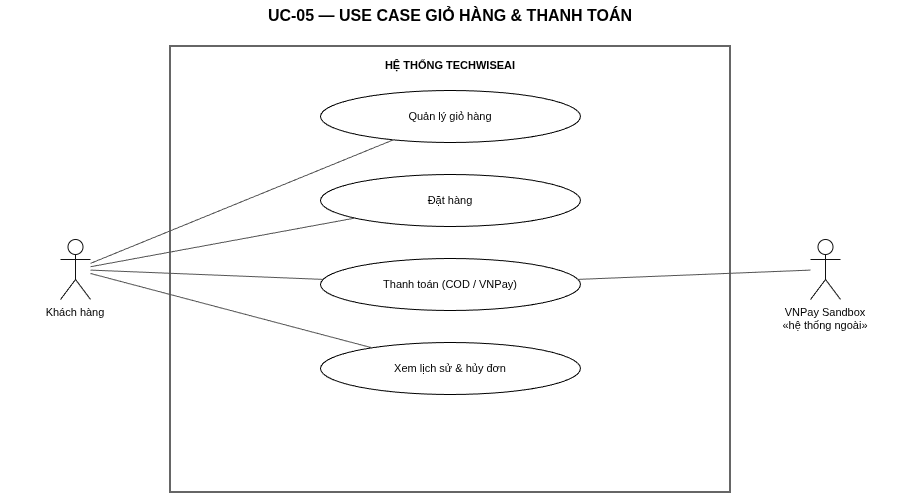
\includegraphics[width=\textwidth]{Image/UC-05_Gio_hang_Thanh_toan.drawio.png}
    \caption{Sơ đồ Use Case giỏ hàng và thanh toán}
    \label{fig:uc-thanh-toan}
\end{figure}

\subsection{Phân tích chức năng tin tức và bài viết}

Nhóm chức năng tin tức cho phép người dùng xem danh sách và nội dung chi tiết các bài viết được công khai trên website.

Hệ thống hiển thị những thông tin như tiêu đề, hình ảnh đại diện, nội dung và thời gian đăng tải, giúp người dùng tiếp cận các thông tin tham khảo về sản phẩm công nghệ.

\begin{figure}[H]
    \centering
    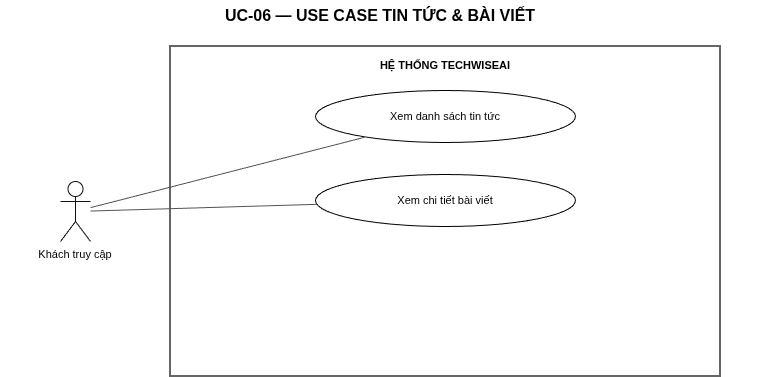
\includegraphics[width=\textwidth]{Image/UC-06_Tin_tuc_Bai_viet.drawio.png}
    \caption{Sơ đồ Use Case tin tức và bài viết}
    \label{fig:uc-tin-tuc}
\end{figure}

\subsection{Phân tích chức năng quản trị hệ thống}

Nhóm chức năng quản trị dành cho Administrator, bao gồm thống kê kho hàng, quản lý sản phẩm, hình ảnh, danh mục, đơn hàng, người dùng, đánh giá và bài viết.

Quản trị viên có thể thêm, cập nhật và quản lý dữ liệu sản phẩm; theo dõi trạng thái đơn hàng; kiểm duyệt đánh giá và quản lý nội dung website. Hình ảnh sản phẩm được quản lý thông qua dịch vụ Cloudinary.

\begin{figure}[H]
    \centering
    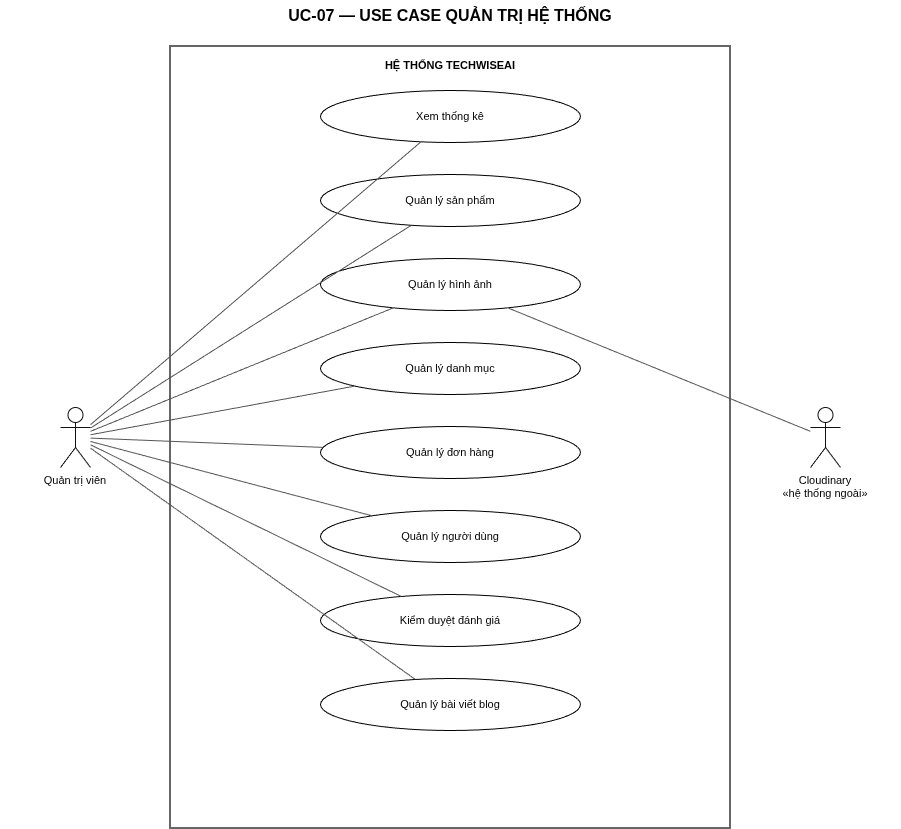
\includegraphics[width=\textwidth]{Image/UC-07_Quan_tri_Admin.drawio.png}
    \caption{Sơ đồ Use Case quản trị hệ thống}
    \label{fig:uc-quan-tri}
\end{figure}

\section{Thiết kế kiến trúc hệ thống}
Kiến trúc hệ thống đóng vai trò quan trọng trong quá trình
phát triển phần mềm, quyết định cách thức tổ chức các thành
phần, phân chia trách nhiệm xử lý và thiết lập cơ chế giao
tiếp giữa các bộ phận. Đối với hệ thống thương mại điện tử
TechWiseAI, việc thiết kế kiến trúc không chỉ cần đáp ứng
các chức năng nghiệp vụ thông thường mà còn phải hỗ trợ
tích hợp các mô hình trí tuệ nhân tạo phục vụ tìm kiếm,
tư vấn và đề xuất sản phẩm.\\\\
Trên cơ sở các yêu cầu đã phân tích, hệ thống được thiết
kế theo hướng phân tách các thành phần giao diện người dùng,
xử lý nghiệp vụ, xử lý trí tuệ nhân tạo và lưu trữ dữ liệu.
Mỗi thành phần đảm nhiệm một nhóm chức năng cụ thể và
giao tiếp thông qua các giao diện được xác định rõ ràng.\\\\
Cách tổ chức này nhằm hạn chế sự phụ thuộc trực tiếp giữa
các thành phần, đồng thời tạo điều kiện thuận lợi cho việc
phát triển, kiểm thử, bảo trì và mở rộng hệ thống trong
tương lai.

\subsection{Kiến trúc tổng thể hệ thống}
Hệ thống TechWiseAI được thiết kế theo mô hình kiến trúc
phân tầng kết hợp với việc tách riêng dịch vụ xử lý trí
tuệ nhân tạo. Kiến trúc tổng thể bao gồm tầng giao diện
người dùng, tầng xử lý nghiệp vụ, tầng dịch vụ trí tuệ
nhân tạo và tầng lưu trữ dữ liệu. Bên cạnh đó, hệ thống
còn tích hợp một số dịch vụ bên ngoài nhằm hỗ trợ các
chức năng chuyên biệt.\\\\
Tầng giao diện người dùng được xây dựng bằng Next.js,
đảm nhiệm việc hiển thị thông tin và tiếp nhận các thao
tác từ người sử dụng. Các yêu cầu phát sinh từ giao diện
được chuyển đến hệ thống backend để thực hiện xử lý.\\\\
Tầng xử lý nghiệp vụ được phát triển bằng Spring Boot,
đóng vai trò trung tâm trong việc quản lý các chức năng
thương mại điện tử. Thành phần này chịu trách nhiệm xử
lý các yêu cầu liên quan đến tài khoản, sản phẩm, giỏ
hàng, đơn hàng, thanh toán và những nghiệp vụ khác.\\\\
Đối với các chức năng có sử dụng trí tuệ nhân tạo, hệ
thống tổ chức một dịch vụ riêng được phát triển bằng
FastAPI. Dịch vụ này đảm nhiệm việc xử lý các yêu cầu
tư vấn sản phẩm bằng chatbot, tìm kiếm sản phẩm dựa trên
hình ảnh và đề xuất sản phẩm theo hành vi người dùng.\\\\
Tầng lưu trữ dữ liệu sử dụng hệ quản trị cơ sở dữ liệu
PostgreSQL kết hợp với phần mở rộng pgvector. Ngoài việc
lưu trữ dữ liệu nghiệp vụ, hệ thống còn có khả năng lưu
trữ và thực hiện các phép toán tìm kiếm trên dữ liệu
vector phục vụ các chức năng trí tuệ nhân tạo.
\begin{figure}[H]
    \centering
    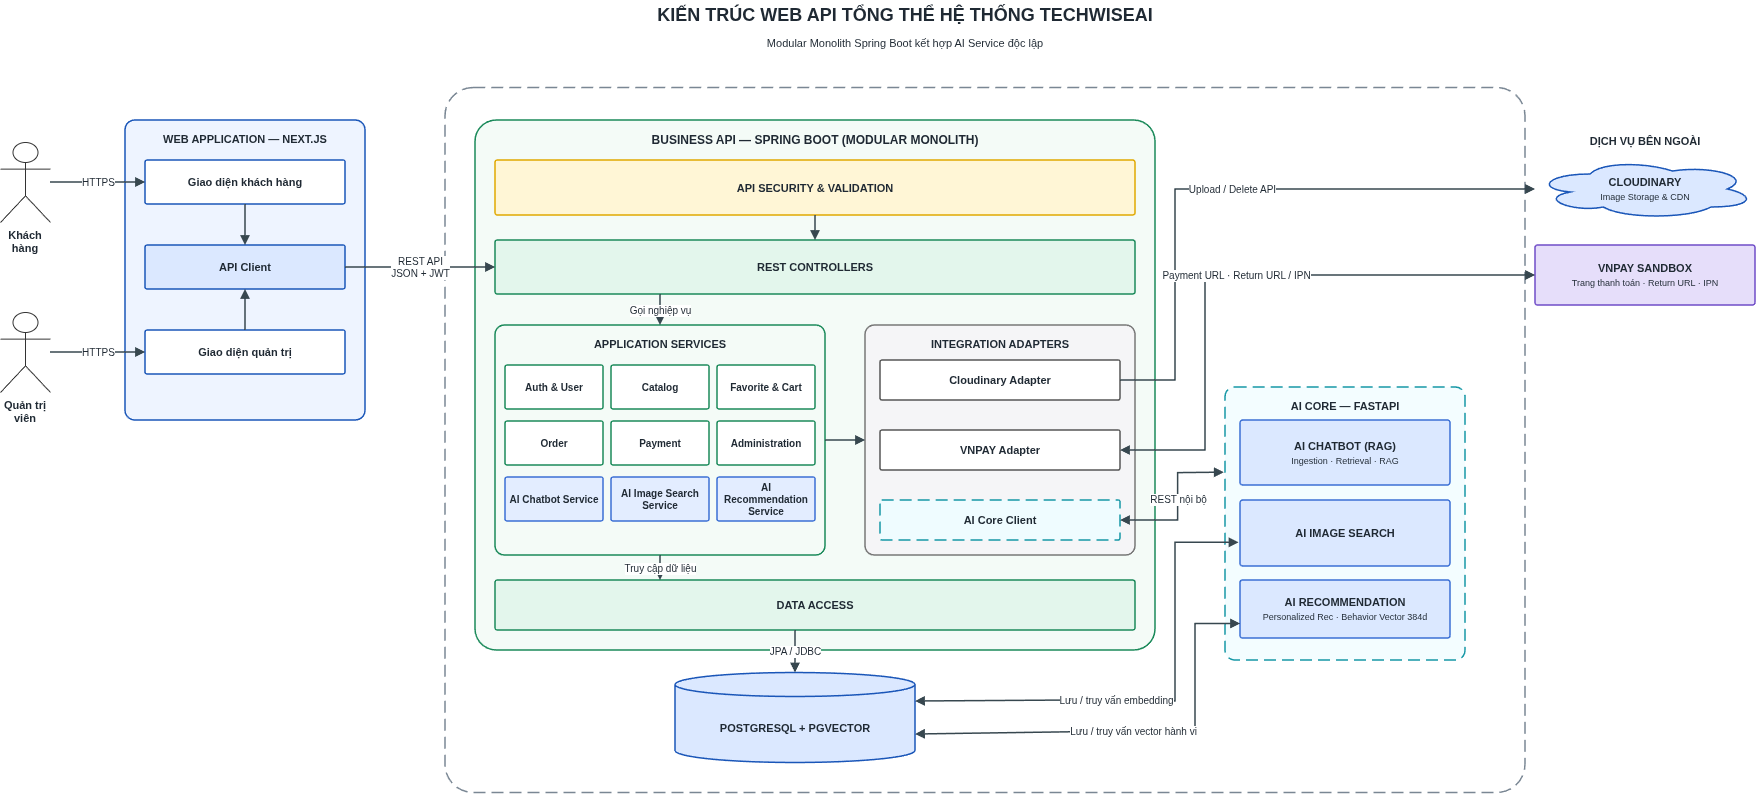
\includegraphics[width=\textwidth]
    {Image/Kien_truc_tong_the_TechWiseAI.drawio.png}
    \caption{Kiến trúc tổng thể hệ thống TechWiseAI}
    \label{fig:system-architecture}
\end{figure}
Việc phân chia thành các thành phần có trách nhiệm riêng
biệt giúp hệ thống duy trì sự độc lập tương đối giữa
phần xử lý nghiệp vụ và phần xử lý trí tuệ nhân tạo.
Nhờ đó, các mô hình AI có thể được thay đổi hoặc nâng
cấp mà không cần điều chỉnh đáng kể cấu trúc của hệ
thống thương mại điện tử.\\\\

\subsection{Thiết kế tầng giao diện người dùng}
Tầng giao diện người dùng là thành phần trực tiếp tương
tác với khách hàng và quản trị viên. Trong hệ thống
TechWiseAI, tầng này được phát triển bằng Next.js dựa
trên thư viện React và ngôn ngữ TypeScript.\\\\
Việc sử dụng Next.js cho phép tổ chức giao diện theo
các thành phần có khả năng tái sử dụng, đồng thời hỗ
trợ xây dựng các trang và luồng điều hướng phù hợp với
đặc điểm của một website thương mại điện tử.\\\\
Giao diện người dùng được phân chia thành hai nhóm
chức năng chính: giao diện dành cho khách hàng và
giao diện dành cho quản trị viên.\\\\
Đối với khách hàng, hệ thống cung cấp các chức năng
như xem danh sách sản phẩm, tìm kiếm, lọc sản phẩm,
xem thông tin chi tiết, quản lý giỏ hàng, đặt hàng
và theo dõi thông tin đơn hàng. Ngoài ra, người dùng
có thể tương tác với các chức năng trí tuệ nhân tạo
được tích hợp trong website.\\\\
Đối với quản trị viên, giao diện cung cấp các chức
năng phục vụ công tác quản lý dữ liệu và vận hành
hệ thống, bao gồm quản lý sản phẩm, danh mục, đơn
hàng, tài khoản và các nội dung liên quan.\\\\
Tầng giao diện không trực tiếp thực hiện các nghiệp
vụ quan trọng hoặc truy cập cơ sở dữ liệu. Thay vào
đó, các yêu cầu được gửi đến backend thông qua các
giao diện lập trình ứng dụng.\\\\
Cách tổ chức này giúp tách biệt trách nhiệm hiển thị
và xử lý dữ liệu, đồng thời hạn chế việc đưa các
thông tin cấu hình hoặc logic nghiệp vụ nhạy cảm
vào phía trình duyệt.

\subsection{Thiết kế tầng xử lý nghiệp vụ}
Tầng xử lý nghiệp vụ được xây dựng bằng Java và
Spring Boot, đóng vai trò trung tâm trong kiến trúc
hệ thống TechWiseAI.\\\\
Thành phần này được tổ chức theo hướng kiến trúc
nguyên khối có phân chia module
(\textit{Modular Monolith}). Theo đó, các chức năng
nghiệp vụ được triển khai trong cùng một ứng dụng
backend nhưng được phân chia thành những module
có trách nhiệm tương đối độc lập.\\\\
Cách tiếp cận này phù hợp với phạm vi của hệ thống,
giúp đơn giản hóa quá trình phát triển và triển khai,
đồng thời vẫn duy trì khả năng tổ chức và mở rộng
mã nguồn.

\subsubsection{Tổ chức các lớp xử lý}
Trong từng module nghiệp vụ, hệ thống được tổ chức
thành các lớp xử lý với trách nhiệm khác nhau.\\\\
Lớp Controller tiếp nhận các yêu cầu HTTP từ phía
giao diện người dùng, thực hiện ánh xạ yêu cầu đến
các phương thức xử lý và trả về kết quả thông qua
REST API.\\\\
Lớp Service chịu trách nhiệm thực hiện logic nghiệp
vụ, kiểm tra các điều kiện xử lý và phối hợp các
thành phần liên quan để hoàn thành yêu cầu.\\\\
Lớp Repository đảm nhiệm việc truy cập và thao tác
với dữ liệu trong cơ sở dữ liệu PostgreSQL. Thông
qua cơ chế ánh xạ đối tượng -- quan hệ, các thao
tác dữ liệu được thực hiện dựa trên các thực thể
được định nghĩa trong hệ thống.\\\\
Bên cạnh đó, các đối tượng DTO được sử dụng để
trao đổi dữ liệu giữa các lớp và giới hạn những
thông tin được gửi đến phía người dùng.\\\\
Việc phân chia trách nhiệm theo từng lớp giúp mã
nguồn có cấu trúc rõ ràng, thuận lợi cho quá trình
kiểm thử, bảo trì và phát triển thêm chức năng.

\subsubsection{Quản lý xác thực và phân quyền}
Hệ thống sử dụng cơ chế xác thực dựa trên JSON Web
Token (JWT) nhằm quản lý phiên truy cập của người
dùng.\\\\
Sau khi người dùng đăng nhập thành công, backend
thực hiện xác thực thông tin và cấp token phù hợp.
Trong các yêu cầu tiếp theo, token được sử dụng
để xác định danh tính và kiểm tra quyền truy cập
đối với những tài nguyên cần được bảo vệ.\\\\
Cơ chế phân quyền được áp dụng nhằm phân biệt các
chức năng dành cho khách hàng và quản trị viên.
Những thao tác có ảnh hưởng đến dữ liệu quản trị
hoặc thông tin cá nhân phải được kiểm tra quyền
truy cập trước khi thực hiện.\\\\
Đối với chức năng chatbot tư vấn sản phẩm công
khai, hệ thống có thể cho phép người dùng gửi yêu
cầu mà không bắt buộc đăng nhập. Tuy nhiên, các
yêu cầu này vẫn cần được kiểm tra dữ liệu đầu vào
và áp dụng các biện pháp kiểm soát phù hợp.

\subsubsection{Phối hợp xử lý với dịch vụ AI}
Bên cạnh các nghiệp vụ thương mại điện tử, Spring
Boot còn đảm nhiệm vai trò trung gian trong quá
trình giao tiếp giữa giao diện người dùng và dịch
vụ trí tuệ nhân tạo.\\\\
Khi nhận được yêu cầu sử dụng chức năng AI, backend
có thể thực hiện kiểm tra dữ liệu đầu vào và chuyển
tiếp yêu cầu đến dịch vụ FastAPI thông qua giao
tiếp HTTP.\\\\
Kết quả xử lý từ FastAPI được chuyển về backend
để cung cấp cho phía giao diện. Đối với chatbot,
cơ chế truyền dữ liệu dạng luồng có thể được sử
dụng nhằm hiển thị nội dung phản hồi theo quá trình
sinh văn bản.\\\\
Việc tổ chức Spring Boot làm thành phần trung gian
giúp tập trung các chính sách truy cập và hạn chế
việc công khai trực tiếp các địa chỉ dịch vụ AI
nội bộ.

\subsection{Thiết kế tầng dịch vụ trí tuệ nhân tạo}
Tầng dịch vụ trí tuệ nhân tạo được phát triển bằng
Python và FastAPI, hoạt động như một thành phần
xử lý riêng biệt so với backend nghiệp vụ.\\\
Việc sử dụng Python tạo điều kiện thuận lợi cho
quá trình tích hợp các thư viện học máy, xử lý
dữ liệu và thực hiện suy luận bằng các mô hình
trí tuệ nhân tạo.\\\\
Dịch vụ AI của TechWiseAI được tổ chức thành ba
nhóm chức năng chính: chatbot tư vấn sản phẩm,
tìm kiếm sản phẩm bằng hình ảnh và đề xuất sản
phẩm dựa trên hành vi người dùng.

\subsubsection{Module chatbot tư vấn sản phẩm}
Module chatbot được xây dựng dựa trên kiến trúc
Retrieval-Augmented Generation (RAG), kết hợp
khả năng truy xuất dữ liệu sản phẩm với mô hình
ngôn ngữ lớn.\\\\
Khi tiếp nhận câu hỏi, hệ thống thực hiện phân
tích yêu cầu và tìm kiếm những sản phẩm có liên
quan trong cơ sở dữ liệu. Quá trình truy xuất
kết hợp phương pháp tìm kiếm ngữ nghĩa và tìm
kiếm từ khóa nhằm nâng cao khả năng xác định
các sản phẩm phù hợp.\\\\
Mô hình BAAI/bge-m3 được sử dụng để biểu diễn
nội dung văn bản dưới dạng vector embedding.
Các vector được lưu trữ và truy vấn thông qua
PostgreSQL kết hợp pgvector.\\\\
Sau khi thu thập được dữ liệu liên quan, hệ
thống xây dựng ngữ cảnh đầu vào và chuyển đến
mô hình ngôn ngữ Qwen được triển khai cục bộ.\\\\
Qwen đảm nhiệm việc tổng hợp thông tin và sinh
câu trả lời tư vấn dựa trên dữ liệu sản phẩm
được cung cấp. Cách tiếp cận này nhằm hạn chế
việc mô hình tạo ra những thông tin không phù
hợp với dữ liệu hiện có của hệ thống.\\\\
Việc triển khai mô hình ngôn ngữ cục bộ giúp
giảm sự phụ thuộc vào dịch vụ sinh ngôn ngữ
bên ngoài, đồng thời cho phép chủ động kiểm
soát cấu hình suy luận và tài nguyên sử dụng.

\subsubsection{Module tìm kiếm sản phẩm bằng hình ảnh}
Module tìm kiếm bằng hình ảnh cho phép người
dùng cung cấp hình ảnh làm đầu vào để tìm kiếm
những sản phẩm có đặc điểm tương đồng trong
cơ sở dữ liệu.\\\\
Thành phần này đảm nhiệm việc tiếp nhận và
tiền xử lý hình ảnh, trích xuất đặc trưng
phù hợp và thực hiện đối sánh với dữ liệu
sản phẩm đã được lưu trữ.\\\\
Kết quả tìm kiếm được biểu diễn dưới dạng
danh sách sản phẩm có mức độ tương đồng
phù hợp với hình ảnh đầu vào.\\\\
Việc tách riêng module tìm kiếm hình ảnh
giúp hệ thống có thể thay đổi mô hình xử
lý hình ảnh mà không ảnh hưởng trực tiếp
đến các chức năng nghiệp vụ khác.

\subsubsection{Module đề xuất sản phẩm}
Module đề xuất sản phẩm được thiết kế nhằm
cung cấp các gợi ý phù hợp với nhu cầu và
hành vi tương tác của người dùng.\\\\
Hệ thống có thể khai thác những thông tin
liên quan đến lịch sử tương tác, sản phẩm
được quan tâm và các đặc trưng của sản
phẩm để xác định mức độ phù hợp.\\\\
Kết quả xử lý của module là danh sách
sản phẩm được sắp xếp theo mức độ ưu
tiên, sau đó được chuyển đến giao diện
để hiển thị cho người dùng.\\\\
Việc tổ chức module đề xuất độc lập với
các module AI khác tạo điều kiện thuận
lợi cho quá trình điều chỉnh phương pháp
xếp hạng và đánh giá chất lượng gợi ý.\\\\
Các thuật toán, quy trình xử lý và sơ đồ
thiết kế chi tiết của từng module AI
sẽ được trình bày trong Mục 3.5.

\subsection{Thiết kế tầng lưu trữ dữ liệu}
Tầng lưu trữ dữ liệu được xây dựng trên
hệ quản trị cơ sở dữ liệu quan hệ
PostgreSQL, kết hợp phần mở rộng pgvector
để hỗ trợ các thao tác với dữ liệu vector.\\\\
PostgreSQL được sử dụng để quản lý dữ
liệu nghiệp vụ của hệ thống thương mại
điện tử, bao gồm thông tin người dùng,
sản phẩm, danh mục, giỏ hàng, đơn hàng
và những dữ liệu liên quan.\\\\
Dữ liệu được tổ chức theo mô hình quan
hệ, sử dụng các khóa và ràng buộc nhằm
đảm bảo tính nhất quán trong quá trình
lưu trữ và cập nhật.\\\\
Bên cạnh dữ liệu nghiệp vụ, hệ thống
còn lưu trữ dữ liệu phục vụ các chức
năng trí tuệ nhân tạo.\\\\
Đối với chatbot RAG, thông tin sản phẩm
được biểu diễn dưới dạng tài liệu văn
bản và vector embedding. Các vector
này được sử dụng để thực hiện truy
vấn tìm kiếm ngữ nghĩa.\\\\
Phần mở rộng pgvector cho phép lưu trữ
vector trực tiếp trong PostgreSQL và
hỗ trợ các phép toán đo độ tương đồng
phục vụ quá trình truy xuất.\\\\
Việc sử dụng PostgreSQL kết hợp pgvector
giúp hệ thống khai thác dữ liệu quan
hệ và dữ liệu vector trên cùng một
nền tảng lưu trữ, qua đó hạn chế
nhu cầu triển khai thêm một hệ quản
trị cơ sở dữ liệu vector riêng biệt.\\\\
Tuy nhiên, dữ liệu nghiệp vụ và dữ
liệu phục vụ AI vẫn cần được tổ chức
hợp lý để tránh ảnh hưởng không cần
thiết đến hiệu năng truy vấn.\\\\
Thiết kế chi tiết các bảng, thuộc
tính, khóa và mối quan hệ dữ liệu
sẽ được trình bày trong Mục 3.4.

\subsection{Thiết kế tích hợp dịch vụ bên ngoài}
Ngoài các thành phần được phát triển
trực tiếp, hệ thống TechWiseAI còn
tích hợp các dịch vụ bên ngoài nhằm
hỗ trợ những chức năng chuyên biệt.\\\\
Các dịch vụ này được kết nối thông
qua những giao diện lập trình ứng
dụng tương ứng và được quản lý tại
các thành phần backend phù hợp.

\subsubsection{Dịch vụ quản lý hình ảnh Cloudinary}
Cloudinary được sử dụng nhằm hỗ trợ
quản lý và lưu trữ tài nguyên hình
ảnh của hệ thống.\\\\
Trong các nghiệp vụ liên quan đến
hình ảnh sản phẩm, backend thực hiện
phối hợp với Cloudinary để xử lý
việc tải lên và quản lý tài nguyên.\\\\
Thông tin tham chiếu đến hình ảnh
được lưu trong cơ sở dữ liệu nhằm
liên kết tài nguyên hình ảnh với
các đối tượng nghiệp vụ tương ứng.\\\\
Việc sử dụng dịch vụ lưu trữ hình
ảnh riêng giúp giảm nhu cầu lưu
trữ trực tiếp các tệp hình ảnh
trong cơ sở dữ liệu quan hệ.

\subsubsection{Dịch vụ thanh toán VNPay}
Đối với chức năng thanh toán trực
tuyến, hệ thống tích hợp cổng thanh
toán VNPay.\\\\
Spring Boot đảm nhiệm việc chuẩn
bị thông tin giao dịch, tạo yêu
cầu thanh toán và phối hợp với
cổng thanh toán theo quy trình
được hỗ trợ.\\\\
Sau khi giao dịch được xử lý,
backend thực hiện kiểm tra thông
tin phản hồi và cập nhật trạng
thái đơn hàng theo kết quả hợp lệ.\\\\
Việc xử lý thông tin thanh toán
được thực hiện tại backend nhằm
hạn chế việc đưa các thông tin
cấu hình nhạy cảm xuống phía
giao diện người dùng.

\subsection{Cơ chế giao tiếp giữa các thành phần}
Các thành phần trong hệ thống
TechWiseAI được kết nối thông
qua các giao diện giao tiếp
được xác định rõ ràng.\\\\
Đối với những chức năng thương
mại điện tử thông thường, luồng
xử lý bắt đầu khi người dùng
thực hiện thao tác trên giao
diện Next.js.\\\\
Yêu cầu được gửi đến REST API
của Spring Boot. Backend tiến
hành kiểm tra dữ liệu, xác
thực và phân quyền khi cần
thiết, thực hiện nghiệp vụ
và truy cập cơ sở dữ liệu
PostgreSQL.\\\\
Sau khi hoàn thành quá trình
xử lý, backend trả kết quả
về giao diện để cập nhật
thông tin hiển thị.\\\\
Đối với những chức năng AI,
Spring Boot tiếp nhận yêu
cầu từ frontend và chuyển
tiếp đến dịch vụ FastAPI.\\\\
FastAPI thực hiện các bước
xử lý tương ứng với từng
chức năng, có thể bao gồm
tiền xử lý dữ liệu, truy
xuất thông tin, suy luận
mô hình và tổng hợp kết quả.\\\\
Kết quả xử lý được chuyển
trở lại Spring Boot trước
khi cung cấp cho giao diện
người dùng.\\\\
Riêng đối với chatbot RAG,
quá trình sinh câu trả lời
có thể được thực hiện theo
cơ chế truyền dữ liệu dạng
luồng. Cơ chế này cho phép
nội dung phản hồi được hiển
thị từng phần thay vì phải
chờ toàn bộ câu trả lời
được tạo xong.\\\\
Trong quá trình giao tiếp
giữa các thành phần, hệ
thống cần chú trọng việc
kiểm tra dữ liệu đầu vào,
xử lý ngoại lệ, kiểm soát
thời gian chờ và bảo vệ
các giao diện dịch vụ
không dành cho truy cập
công khai.\\\\
Nhìn chung, kiến trúc được
thiết kế theo hướng phân
chia trách nhiệm rõ ràng
giữa giao diện, nghiệp vụ,
dịch vụ AI và lưu trữ dữ
liệu. Cách tổ chức này tạo
nền tảng cho việc triển
khai các chức năng thương
mại điện tử kết hợp trí
tuệ nhân tạo, đồng thời
hỗ trợ quá trình bảo trì
và mở rộng hệ thống.


\section{Thiết kế cơ sở dữ liệu}
Cơ sở dữ liệu TechWiseAI được xây dựng bằng PostgreSQL, kết hợp phần mở rộng pgvector nhằm đáp ứng yêu cầu lưu trữ dữ liệu nghiệp vụ và dữ liệu phục vụ trí tuệ nhân tạo.\\\\
PostgreSQL hỗ trợ quản lý dữ liệu quan hệ, bảo đảm tính toàn vẹn và nhất quán trong các giao dịch. Trong khi đó, pgvector cho phép lưu trữ và truy vấn vector embedding, phục vụ chatbot RAG, tìm kiếm sản phẩm bằng hình ảnh và hệ thống gợi ý cá nhân hóa.

\subsection{Tổng quan thiết kế cơ sở dữ liệu}
Cơ sở dữ liệu được thiết kế theo mô hình quan hệ, sử dụng khóa chính (Primary Key) và khóa ngoại (Foreign Key) để xác định các thực thể và mối liên kết giữa chúng.\\\\
Thiết kế hướng đến các mục tiêu chính:
\begin{itemize}
    \item Đáp ứng yêu cầu lưu trữ dữ liệu cho các chức năng thương mại điện tử.
    \item Hạn chế trùng lặp và bảo đảm tính toàn vẹn dữ liệu.
    \item Hỗ trợ truy vấn, tìm kiếm và quản lý sản phẩm hiệu quả.
    \item Lưu trữ dữ liệu vector phục vụ các chức năng AI.
    \item Tạo điều kiện thuận lợi cho việc bảo trì và mở rộng hệ thống.
\end{itemize}
Các bảng dữ liệu được tổ chức thành những nhóm chính gồm: tài khoản và phân quyền, sản phẩm và danh mục, giỏ hàng và yêu thích, đơn hàng và thanh toán, đánh giá và tương tác, bài viết và nội dung, dữ liệu trí tuệ nhân tạo và dữ liệu hỗ trợ vận hành.

\subsection{Sơ đồ thực thể -- liên kết}
Sơ đồ thực thể -- liên kết (Entity Relationship Diagram -- ERD) mô tả cấu trúc các bảng, thuộc tính, khóa chính, khóa ngoại và mối quan hệ giữa các thực thể trong hệ thống.\\\\
Trong TechWiseAI, bảng \texttt{products} giữ vai trò trung tâm, liên kết với danh mục, hình ảnh, giỏ hàng, đơn hàng, đánh giá và dữ liệu embedding. Bảng \texttt{users} liên kết với các dữ liệu tài khoản, đơn hàng, tương tác và hồ sơ sở thích người dùng.\\\\
Các quan hệ một -- nhiều được biểu diễn thông qua khóa ngoại. Đối với quan hệ nhiều -- nhiều, hệ thống sử dụng các bảng trung gian như \texttt{user\_roles}, \texttt{favorites} và \texttt{blog\_category\_mappings}.
\begin{figure}[p]
    \centering
    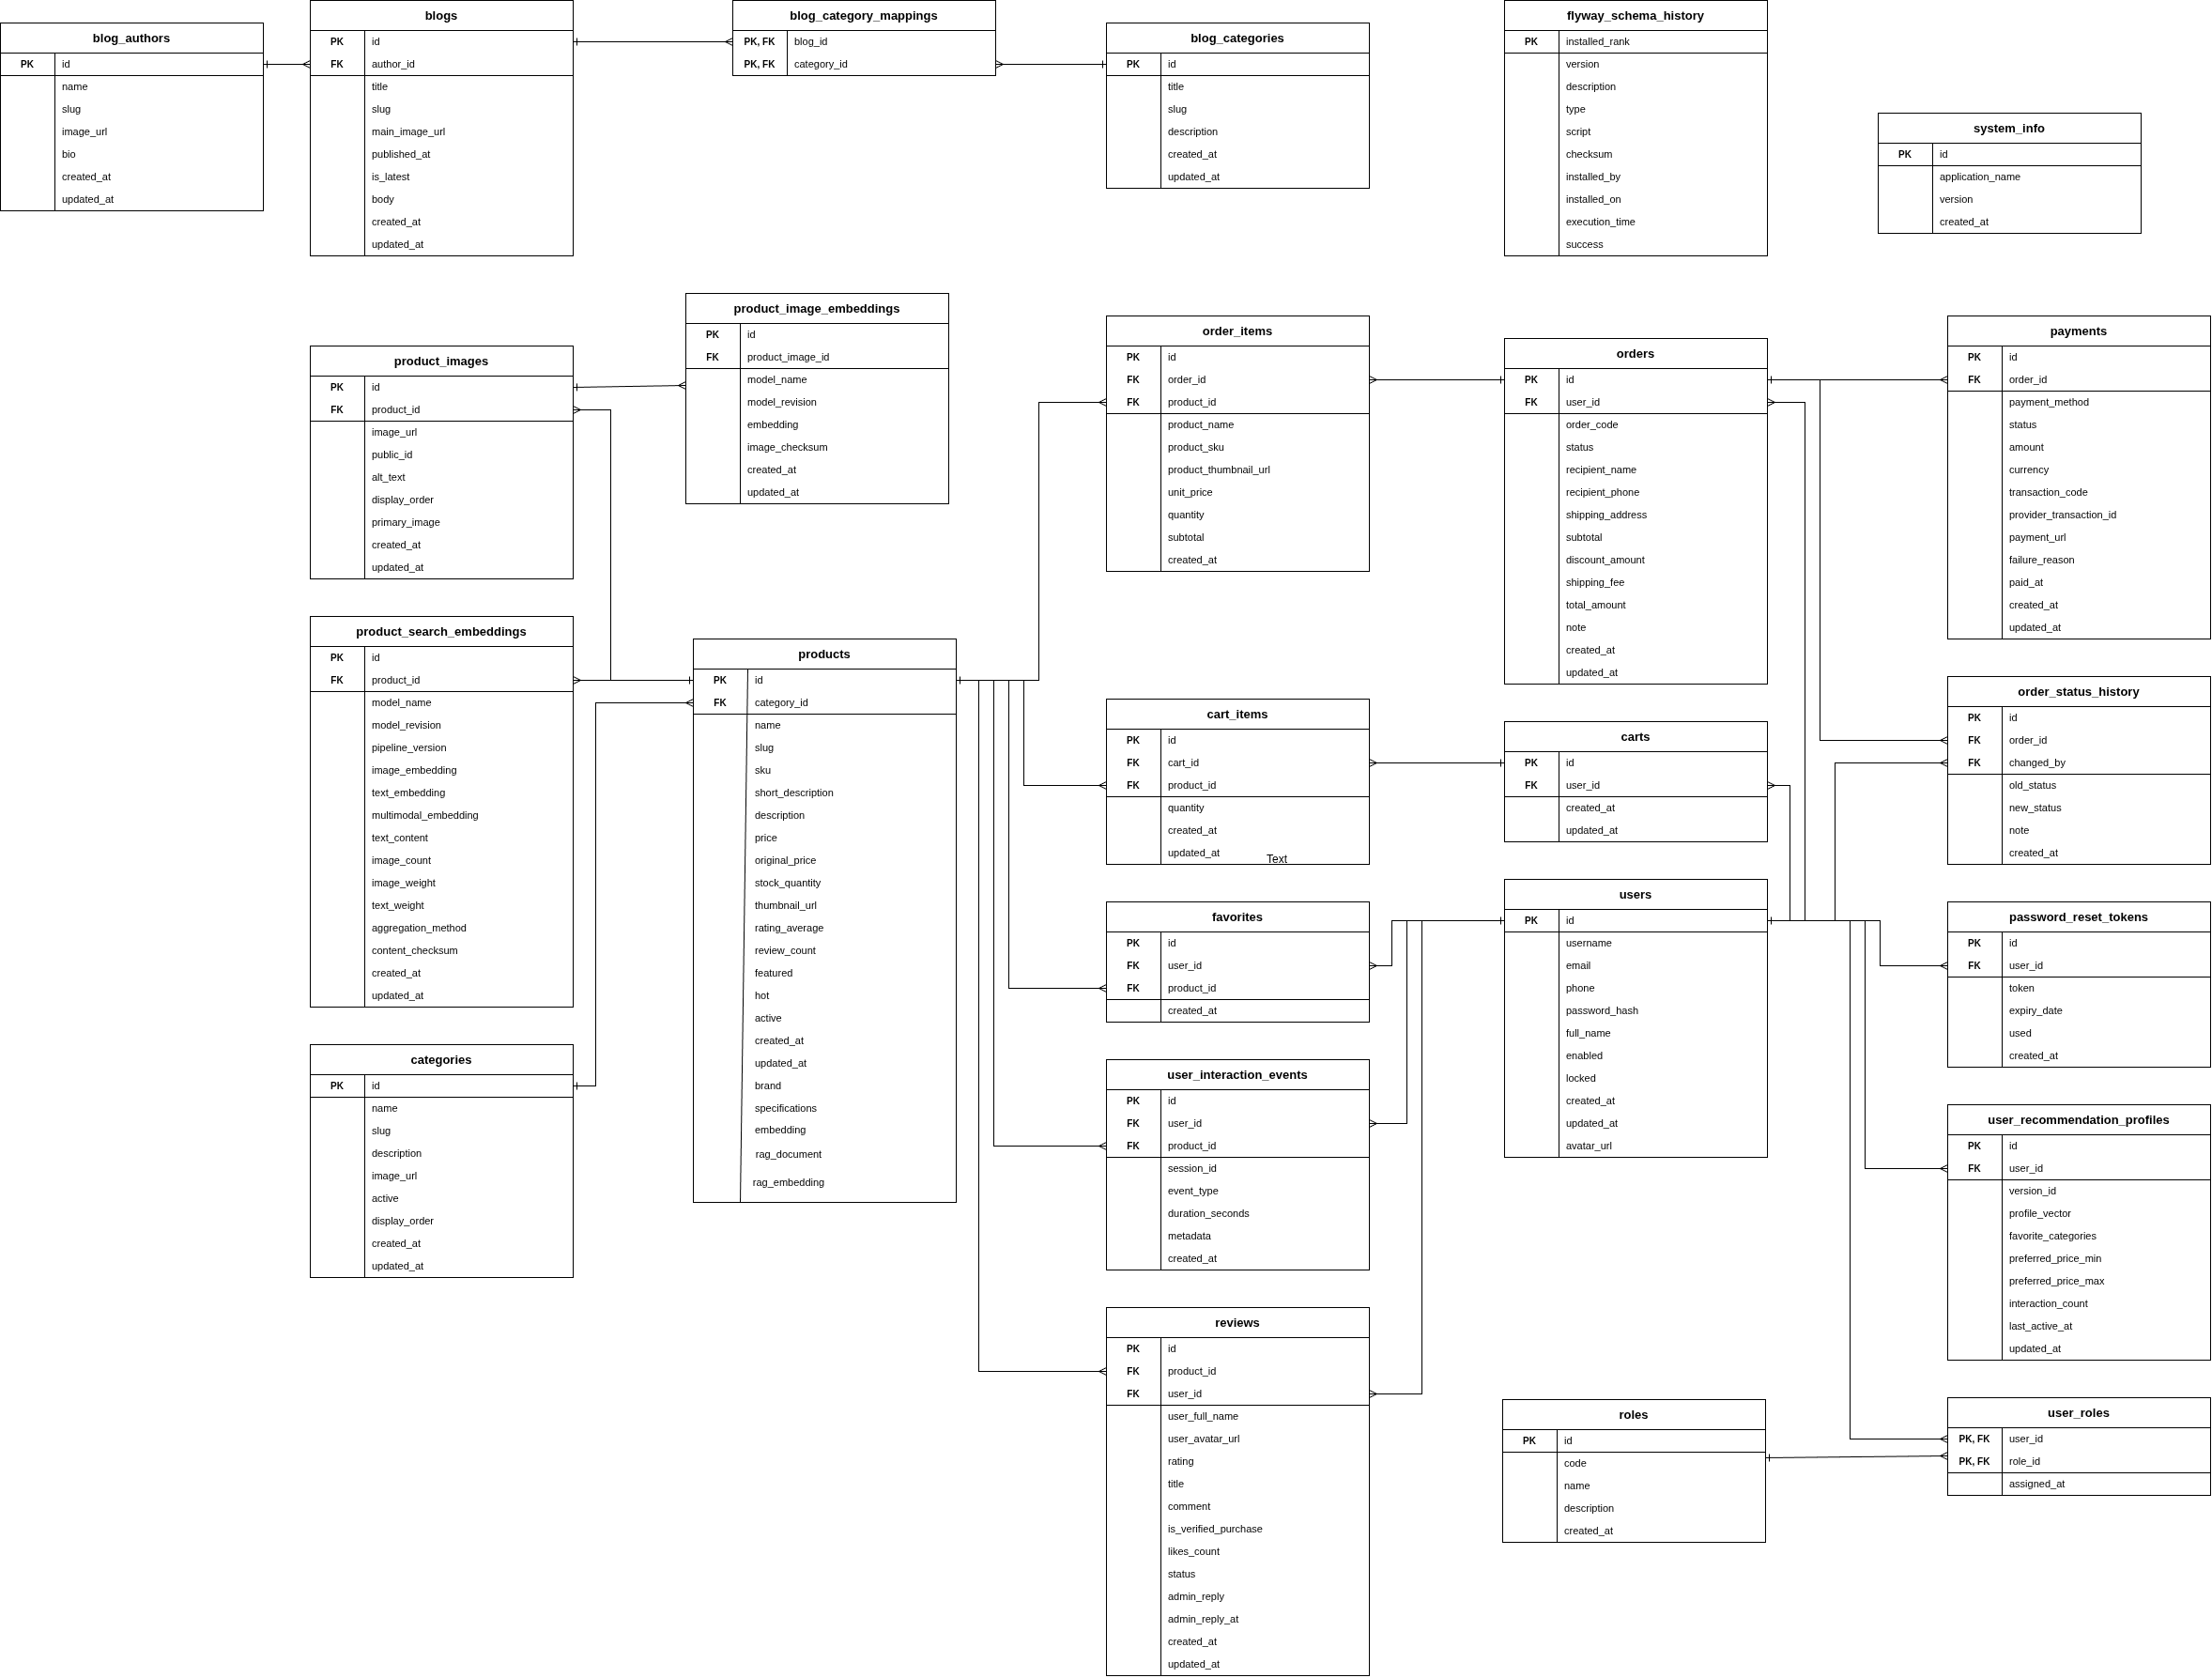
\includegraphics[
        width=\textwidth,
        height=0.85\textheight,
        keepaspectratio
    ]{Image/ERD_TechwiseAI.drawio.png}
    \caption{Sơ đồ thực thể -- liên kết của hệ thống TechWiseAI}
    \label{fig:techwiseai-erd}
\end{figure}

\subsection{Thiết kế các nhóm bảng dữ liệu nghiệp vụ}
\subsubsection{Nhóm quản lý tài khoản và phân quyền}
Nhóm này bao gồm các bảng \texttt{users}, \texttt{roles}, \texttt{user\_roles} và \texttt{password\_reset\_tokens}.\\\\
Bảng \texttt{users} lưu trữ thông tin tài khoản, mật khẩu đã băm, thông tin cá nhân và trạng thái hoạt động. Bảng \texttt{roles} quản lý các vai trò, trong khi \texttt{user\_roles} biểu diễn quan hệ nhiều -- nhiều giữa người dùng và vai trò.\\\\
Bảng \texttt{password\_reset\_tokens} lưu trữ token, thời hạn hiệu lực và trạng thái sử dụng để hỗ trợ chức năng khôi phục mật khẩu.\\\\
Cấu trúc này cho phép quản lý tài khoản độc lập với cơ chế phân quyền và hỗ trợ kiểm soát truy cập hệ thống.

\subsubsection{Nhóm quản lý sản phẩm và danh mục}
Nhóm này bao gồm các bảng \texttt{categories}, \texttt{products} và \texttt{product\_images}.\\\\
Bảng \texttt{categories} lưu trữ danh mục sản phẩm. Bảng \texttt{products} quản lý các thông tin như tên sản phẩm, thương hiệu, giá bán, số lượng tồn kho, mô tả, thông số kỹ thuật và trạng thái kinh doanh.\\\\
Mỗi sản phẩm thuộc một danh mục thông qua khóa ngoại \texttt{category\_id}. Một danh mục có thể chứa nhiều sản phẩm.\\\\
Bảng \texttt{product\_images} lưu trữ các hình ảnh liên kết với sản phẩm, bao gồm đường dẫn, mã tài nguyên, thứ tự hiển thị và trạng thái hình ảnh chính.\\\\
Việc tách hình ảnh thành bảng riêng cho phép quản lý nhiều hình ảnh trên cùng một sản phẩm và thuận tiện khi tích hợp dịch vụ lưu trữ hình ảnh.

\subsubsection{Nhóm quản lý giỏ hàng và sản phẩm yêu thích}
Nhóm này gồm các bảng \texttt{carts}, \texttt{cart\_items} và \texttt{favorites}.\\\\
Bảng \texttt{carts} quản lý giỏ hàng của người dùng, trong khi \texttt{cart\_items} lưu trữ danh sách sản phẩm và số lượng tương ứng.\\\\
Bảng \texttt{favorites} biểu diễn quan hệ giữa người dùng và những sản phẩm được đánh dấu yêu thích. Dữ liệu này cũng có thể được khai thác để xác định mức độ quan tâm của người dùng trong hệ thống gợi ý.\\\\

\subsubsection{Nhóm quản lý đơn hàng và thanh toán}
Nhóm này bao gồm các bảng \texttt{orders}, \texttt{order\_items}, \texttt{payments} và \texttt{order\_status\_history}.\\\\
Bảng \texttt{orders} lưu trữ thông tin khách hàng, địa chỉ giao hàng, tổng giá trị và trạng thái đơn hàng.\\\\
Bảng \texttt{order\_items} quản lý các sản phẩm thuộc đơn hàng, bao gồm số lượng, đơn giá và thành tiền. Một số thông tin sản phẩm được lưu tại thời điểm đặt hàng nhằm bảo toàn lịch sử giao dịch khi dữ liệu sản phẩm thay đổi.\\\\
Bảng \texttt{payments} lưu trữ phương thức thanh toán, số tiền, trạng thái và thông tin giao dịch, hỗ trợ cả COD và VNPay.\\\\
Bảng \texttt{order\_status\_history} ghi nhận lịch sử thay đổi trạng thái đơn hàng, phục vụ theo dõi và kiểm tra quá trình xử lý.

\subsubsection{Nhóm quản lý đánh giá và tương tác người dùng}
Nhóm này gồm hai bảng \texttt{reviews} và \texttt{user\_interaction\_events}.\\\\
Bảng \texttt{reviews} lưu trữ điểm đánh giá, nội dung nhận xét, thông tin người đánh giá và trạng thái kiểm duyệt.\\\\
Bảng \texttt{user\_interaction\_events} ghi nhận các hành vi tương tác với sản phẩm như xem, nhấp vào, yêu thích, thêm vào giỏ hàng hoặc mua hàng.\\\\
Các sự kiện có thể bao gồm loại hành vi, thời điểm, thời lượng tương tác và dữ liệu bổ sung. Đây là nguồn dữ liệu phục vụ việc phân tích sở thích và xây dựng hệ thống gợi ý cá nhân hóa.

\subsubsection{Nhóm quản lý bài viết và nội dung}
Nhóm này bao gồm các bảng \texttt{blog\_authors}, \texttt{blogs}, \texttt{blog\_categories} và \texttt{blog\_category\_mappings}.\\\\
Bảng \texttt{blogs} lưu trữ nội dung bài viết, tiêu đề, hình ảnh và trạng thái xuất bản. Bảng \texttt{blog\_authors} quản lý thông tin tác giả, trong khi \texttt{blog\_categories} quản lý các danh mục bài viết.\\\\
Quan hệ nhiều -- nhiều giữa bài viết và danh mục được biểu diễn thông qua bảng \texttt{blog\_category\_mappings}.

\subsection{Thiết kế dữ liệu phục vụ trí tuệ nhân tạo}
Bên cạnh dữ liệu nghiệp vụ, TechWiseAI tổ chức các trường và bảng chuyên biệt để lưu trữ vector embedding, phục vụ chatbot RAG, tìm kiếm hình ảnh và gợi ý sản phẩm.

\subsubsection{Dữ liệu phục vụ chatbot RAG}
Dữ liệu RAG được lưu trữ trực tiếp trong bảng \texttt{products} thông qua hai trường:
\begin{itemize}
    \item \texttt{rag\_document}: Lưu trữ nội dung văn bản được tổng hợp từ thông tin sản phẩm.
    \item \texttt{rag\_embedding}: Lưu trữ vector biểu diễn ngữ nghĩa của nội dung văn bản.
\end{itemize}
TechWiseAI sử dụng mô hình \texttt{BAAI/bge-m3} để tạo embedding văn bản có 1024 chiều, được lưu trữ bằng kiểu dữ liệu \texttt{VECTOR(1024)} của pgvector.\\\\
Khi người dùng gửi câu hỏi, hệ thống chuyển truy vấn thành vector và tìm kiếm các sản phẩm có mức độ tương đồng ngữ nghĩa cao. Kết quả truy xuất được sử dụng làm ngữ cảnh cho chatbot RAG.\\\\
Việc lưu dữ liệu RAG trong bảng \texttt{products} giúp duy trì liên kết trực tiếp giữa thông tin được truy xuất và sản phẩm thực tế trên website.

\subsubsection{Dữ liệu phục vụ tìm kiếm bằng hình ảnh}
Dữ liệu tìm kiếm hình ảnh được tổ chức thông qua hai bảng \texttt{product\_image\_embeddings} và \texttt{product\_search\_embeddings}.\\\\
Bảng \texttt{product\_image\_embeddings} lưu trữ vector đặc trưng của từng hình ảnh sản phẩm, liên kết với bảng \texttt{product\_images}. Ngoài vector, bảng còn lưu thông tin mô hình, phiên bản và thời điểm cập nhật.\\\\
Bảng \texttt{product\_search\_embeddings} liên kết với bảng \texttt{products}, hỗ trợ lưu trữ các biểu diễn đặc trưng ở cấp sản phẩm, bao gồm vector hình ảnh, văn bản và đa phương thức.\\\\
Các trường cấu hình cho phép quản lý phương pháp tổng hợp đặc trưng và thông tin mô hình sử dụng.\\\\
Cấu trúc này hỗ trợ tìm kiếm sản phẩm dựa trên độ tương đồng hình ảnh, đồng thời tạo điều kiện mở rộng sang tìm kiếm đa phương thức.

\subsubsection{Dữ liệu phục vụ gợi ý sản phẩm}
Chức năng gợi ý sử dụng hai bảng chính là \texttt{user\_interaction\_events} và \texttt{user\_recommendation\_profiles}.\\\\
Bảng \texttt{user\_interaction\_events} lưu trữ lịch sử hành vi, trong khi \texttt{user\_recommendation\_profiles} lưu trữ hồ sơ sở thích được tổng hợp từ các tương tác.\\\\
Hồ sơ sở thích bao gồm vector đại diện \texttt{profile\_vector}, danh mục quan tâm, khoảng giá ưu tiên, số lượng tương tác và thời điểm cập nhật.\\\\
Việc tách dữ liệu hành vi và hồ sơ sở thích giúp hệ thống cập nhật thông tin cá nhân hóa mà không ảnh hưởng đến cấu trúc tài khoản người dùng.

\subsubsection{Tổ chức và truy xuất dữ liệu vector}
Phần mở rộng pgvector cho phép lưu trữ và thực hiện các phép toán tương đồng trên dữ liệu vector.\\\\
Đối với tìm kiếm ngữ nghĩa, hệ thống có thể sử dụng khoảng cách Cosine để xác định các vector liên quan đến truy vấn.\\\\
Bên cạnh đó, các thuộc tính quan hệ như danh mục, thương hiệu, giá bán và trạng thái sản phẩm có thể được kết hợp với truy vấn vector để lọc kết quả theo điều kiện nghiệp vụ.\\\\
Để tối ưu truy xuất, cơ sở dữ liệu có thể sử dụng các chỉ mục phù hợp trên khóa ngoại, thuộc tính thường tìm kiếm và dữ liệu vector. Các kỹ thuật lập chỉ mục gần đúng như HNSW có thể được áp dụng khi quy mô dữ liệu tăng lên.\\\\
Dữ liệu embedding cần được tạo mới hoặc cập nhật khi nội dung nguồn thay đổi, nhằm duy trì sự phù hợp giữa dữ liệu AI và thông tin sản phẩm hiện tại.

\section{Thiết kế các chức năng trí tuệ nhân tạo}
Hệ thống TechWiseAI tích hợp ba module trí tuệ nhân tạo
gồm chatbot tư vấn sản phẩm sử dụng RAG, tìm kiếm sản phẩm
bằng hình ảnh và gợi ý sản phẩm cá nhân hóa.
Các module được thiết kế độc lập và sử dụng chung dữ liệu
sản phẩm nhằm nâng cao trải nghiệm mua sắm.\\\\

\subsection{Thiết kế module chatbot RAG}
Module chatbot RAG hỗ trợ người dùng tìm kiếm và lựa chọn
sản phẩm thông qua ngôn ngữ tự nhiên. Hệ thống kết hợp
truy xuất dữ liệu sản phẩm với mô hình ngôn ngữ lớn
để tạo câu trả lời phù hợp với nhu cầu người dùng.

\subsubsection{Sơ đồ Use Case}
Sơ đồ Use Case mô tả các chức năng của module
với hai tác nhân chính là người dùng và quản trị viên.\\\\
Người dùng có thể gửi câu hỏi tư vấn, tiếp tục hội thoại,
nhận câu trả lời, xem sản phẩm được đề xuất và truy cập
thông tin chi tiết sản phẩm. Quản trị viên thực hiện
quản lý dữ liệu RAG, cập nhật thông tin sản phẩm,
quản lý embedding và kiểm tra trạng thái dữ liệu.
\begin{figure}[H]
    \centering
    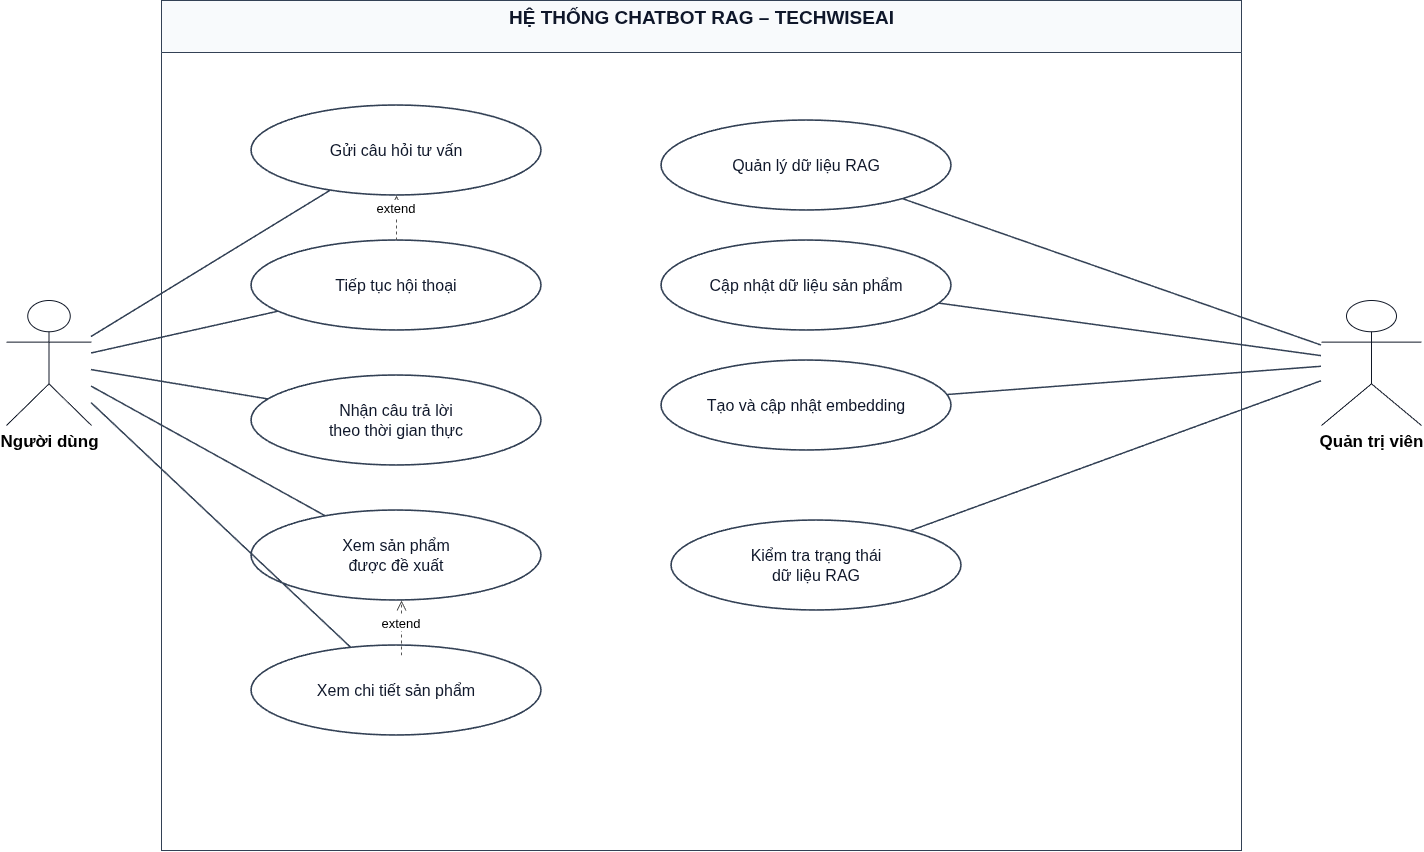
\includegraphics[width=\textwidth]
    {Image/UseCase_Chatbot_RAG_TechWiseAI_Day_Du.drawio}
    \caption{Sơ đồ Use Case module chatbot RAG}
    \label{fig:rag-usecase}
\end{figure}

\subsubsection{Sơ đồ kiến trúc}
Module chatbot RAG gồm các thành phần Query Analyzer,
Embedding Model, Hybrid Retrieval, Context Builder
và LLM Generator.\\\\
Query Analyzer phân tích yêu cầu để xác định danh mục,
thương hiệu và khoảng giá. Mô hình BAAI/bge-m3
chuyển đổi truy vấn thành vector 1024 chiều.
Hybrid Retrieval kết hợp tìm kiếm từ khóa và tìm kiếm
ngữ nghĩa trên PostgreSQL/pgvector, sau đó tổng hợp
kết quả bằng thuật toán Reciprocal Rank Fusion (RRF).\\\\
Thông tin sản phẩm được sử dụng để xây dựng ngữ cảnh
cho mô hình ngôn ngữ sinh câu trả lời.
Kết quả được truyền theo cơ chế streaming
đến giao diện người dùng thông qua Spring Boot.
\begin{figure}[H]
    \centering
    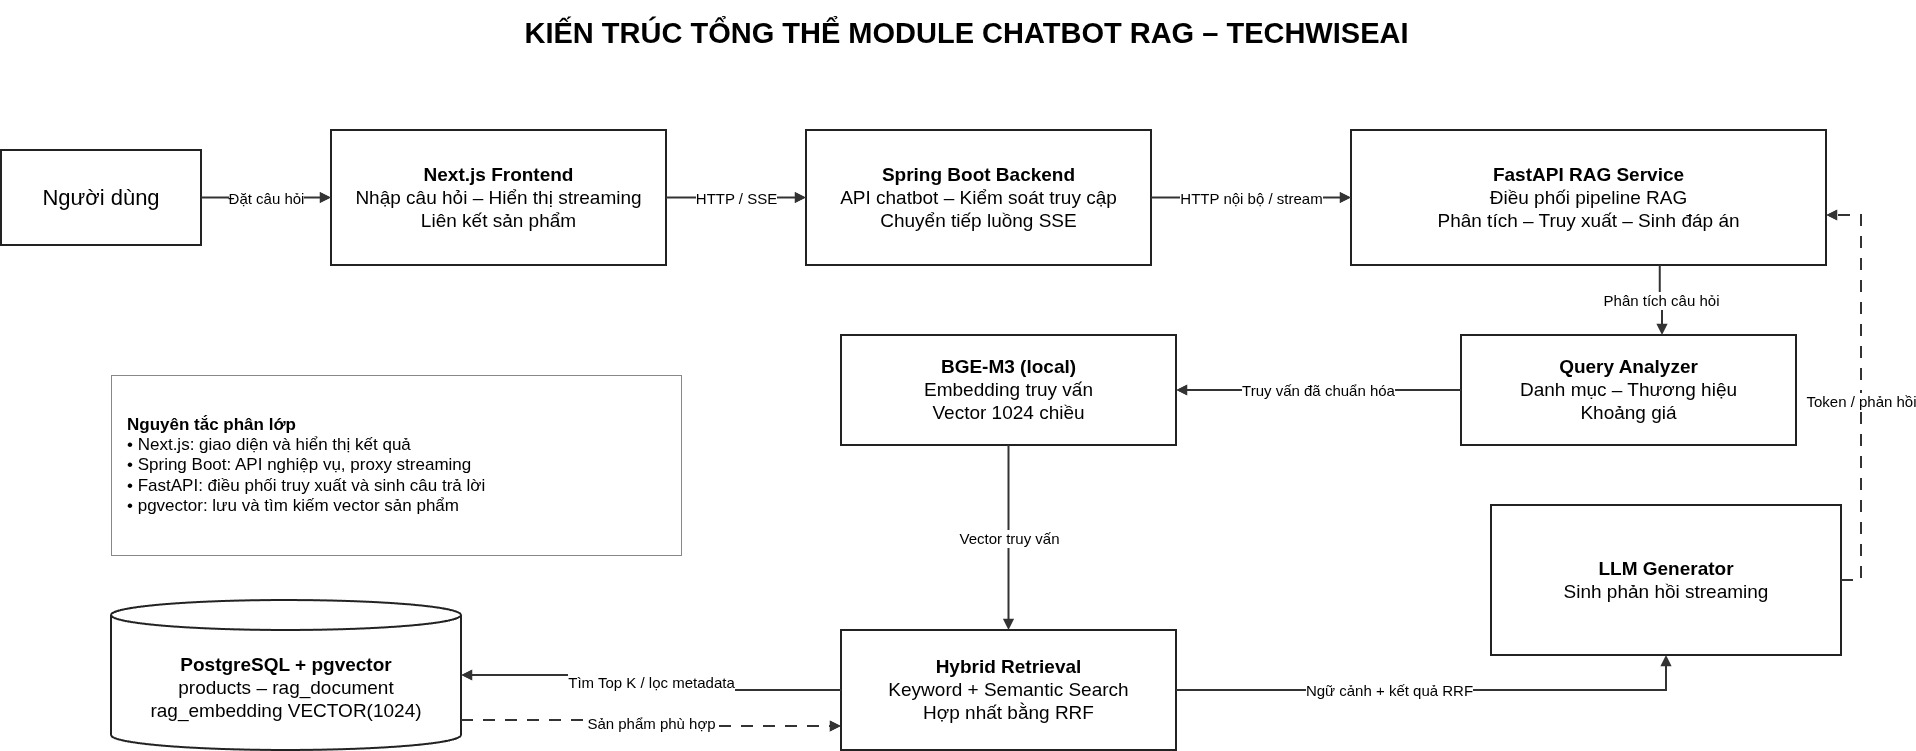
\includegraphics[width=\textwidth]
    {Image/TechWiseAI_Kien_Truc_Tong_The_Chatbot_RAG.drawio.png}
    \caption{Sơ đồ kiến trúc module chatbot RAG}
    \label{fig:rag-architecture}
\end{figure}


\subsubsection{Sơ đồ tuần tự}
Sơ đồ tuần tự mô tả quá trình tương tác giữa
người dùng và các thành phần của hệ thống
khi thực hiện tư vấn sản phẩm bằng chatbot RAG.
Sau khi tiếp nhận câu hỏi, hệ thống phân tích
truy vấn, tạo vector embedding và thực hiện
tìm kiếm kết hợp. Kết quả được hợp nhất bằng
thuật toán RRF, sau đó cung cấp ngữ cảnh
cho mô hình ngôn ngữ để sinh câu trả lời.
Phản hồi được truyền theo cơ chế streaming
đến giao diện người dùng.
\begin{figure}[H]
    \centering
    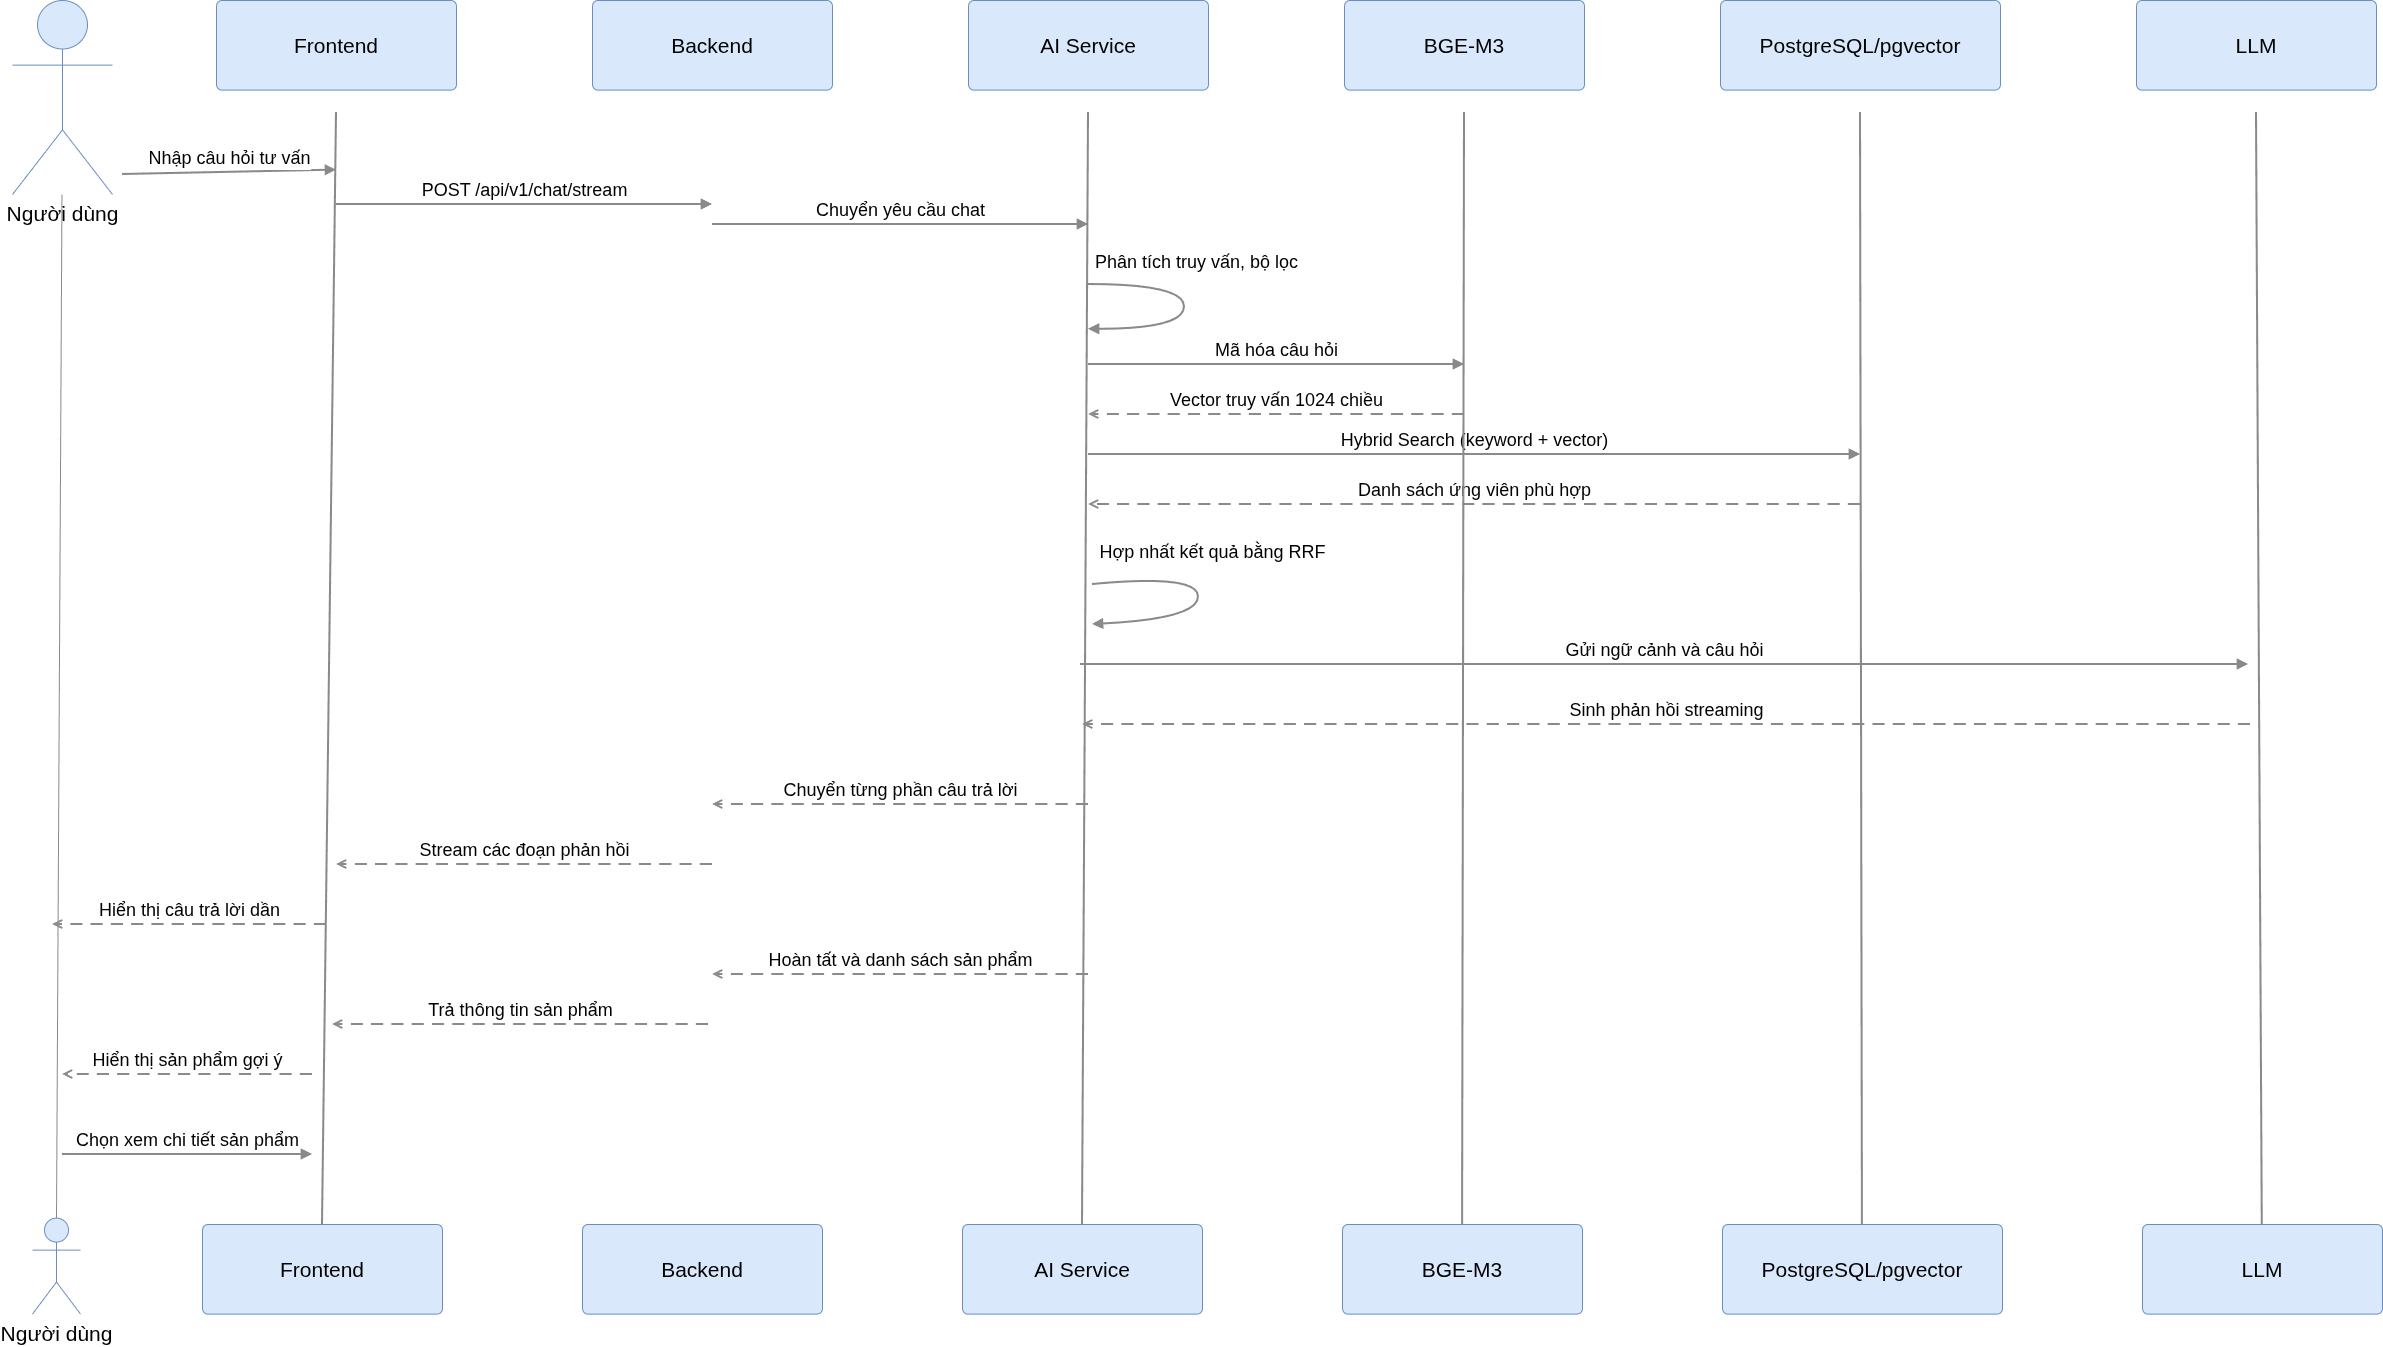
\includegraphics[width=\textwidth]
    {Image/TechWiseAI_Sequence_Chatbot_RAG_Kich_Thuoc_Lon.drawio.png}
    \caption{Sơ đồ tuần tự module chatbot RAG}
    \label{fig:sequence-rag}
\end{figure}

\subsection{Thiết kế module tìm kiếm sản phẩm bằng hình ảnh}
Module tìm kiếm bằng hình ảnh cho phép người dùng
tìm kiếm sản phẩm dựa trên đặc điểm trực quan,
thay vì phải nhập tên hoặc từ khóa mô tả.

\subsubsection{Sơ đồ Use Case}
Sơ đồ Use Case thể hiện các chức năng tương tác
giữa người dùng, quản trị viên và module tìm kiếm.\\\\
Người dùng có thể tải hình ảnh lên, thực hiện tìm kiếm,
xem danh sách sản phẩm tương đồng và truy cập
thông tin chi tiết sản phẩm.\\\\
Quản trị viên thực hiện quản lý dữ liệu hình ảnh,
cập nhật hình ảnh sản phẩm và quản lý dữ liệu
vector phục vụ tìm kiếm.
\begin{figure}[H]
    \centering
    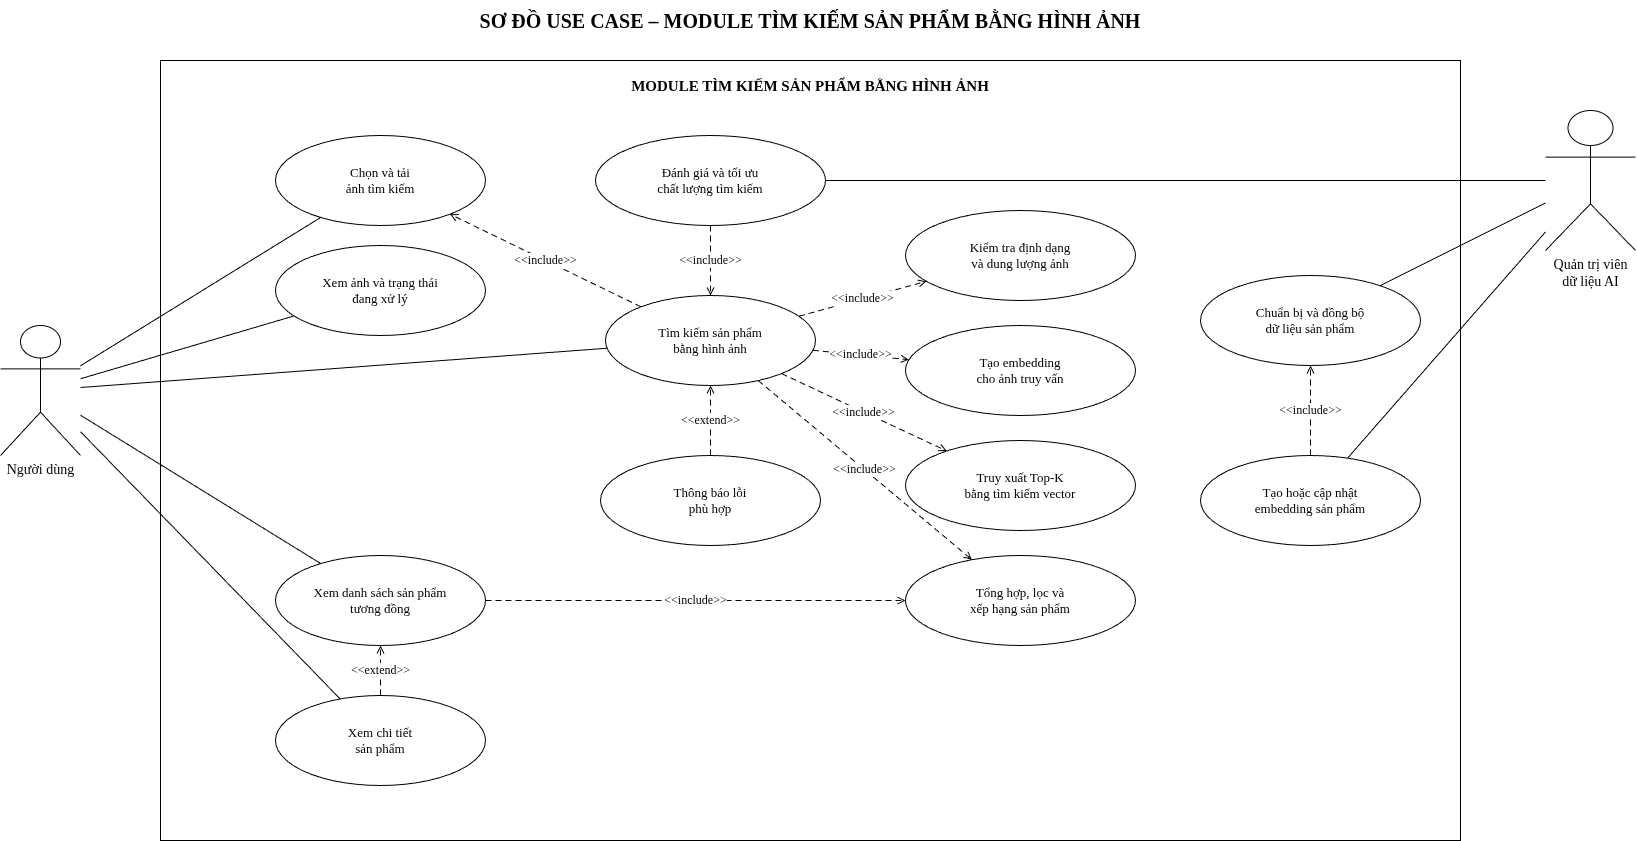
\includegraphics[width=\textwidth]
    {Image/UseCase_TimKiemBangAnh.drawio.png}
    \caption{Sơ đồ Use Case module tìm kiếm bằng hình ảnh}
    \label{fig:image-search-usecase}
\end{figure}

\subsubsection{Sơ đồ kiến trúc}
Module sử dụng mô hình SigLIP để trích xuất đặc trưng
hình ảnh và biểu diễn dưới dạng vector.\\\\
Các vector hình ảnh sản phẩm được lưu trữ
trong PostgreSQL/pgvector và liên kết với dữ liệu
sản phẩm tương ứng.\\\\
Khi người dùng cung cấp hình ảnh, hệ thống thực hiện
tiền xử lý, tạo vector truy vấn và so sánh với
các vector đã lưu. Những sản phẩm có mức độ tương đồng
cao nhất được lựa chọn và trả về giao diện.
\begin{figure}[H]
    \centering
    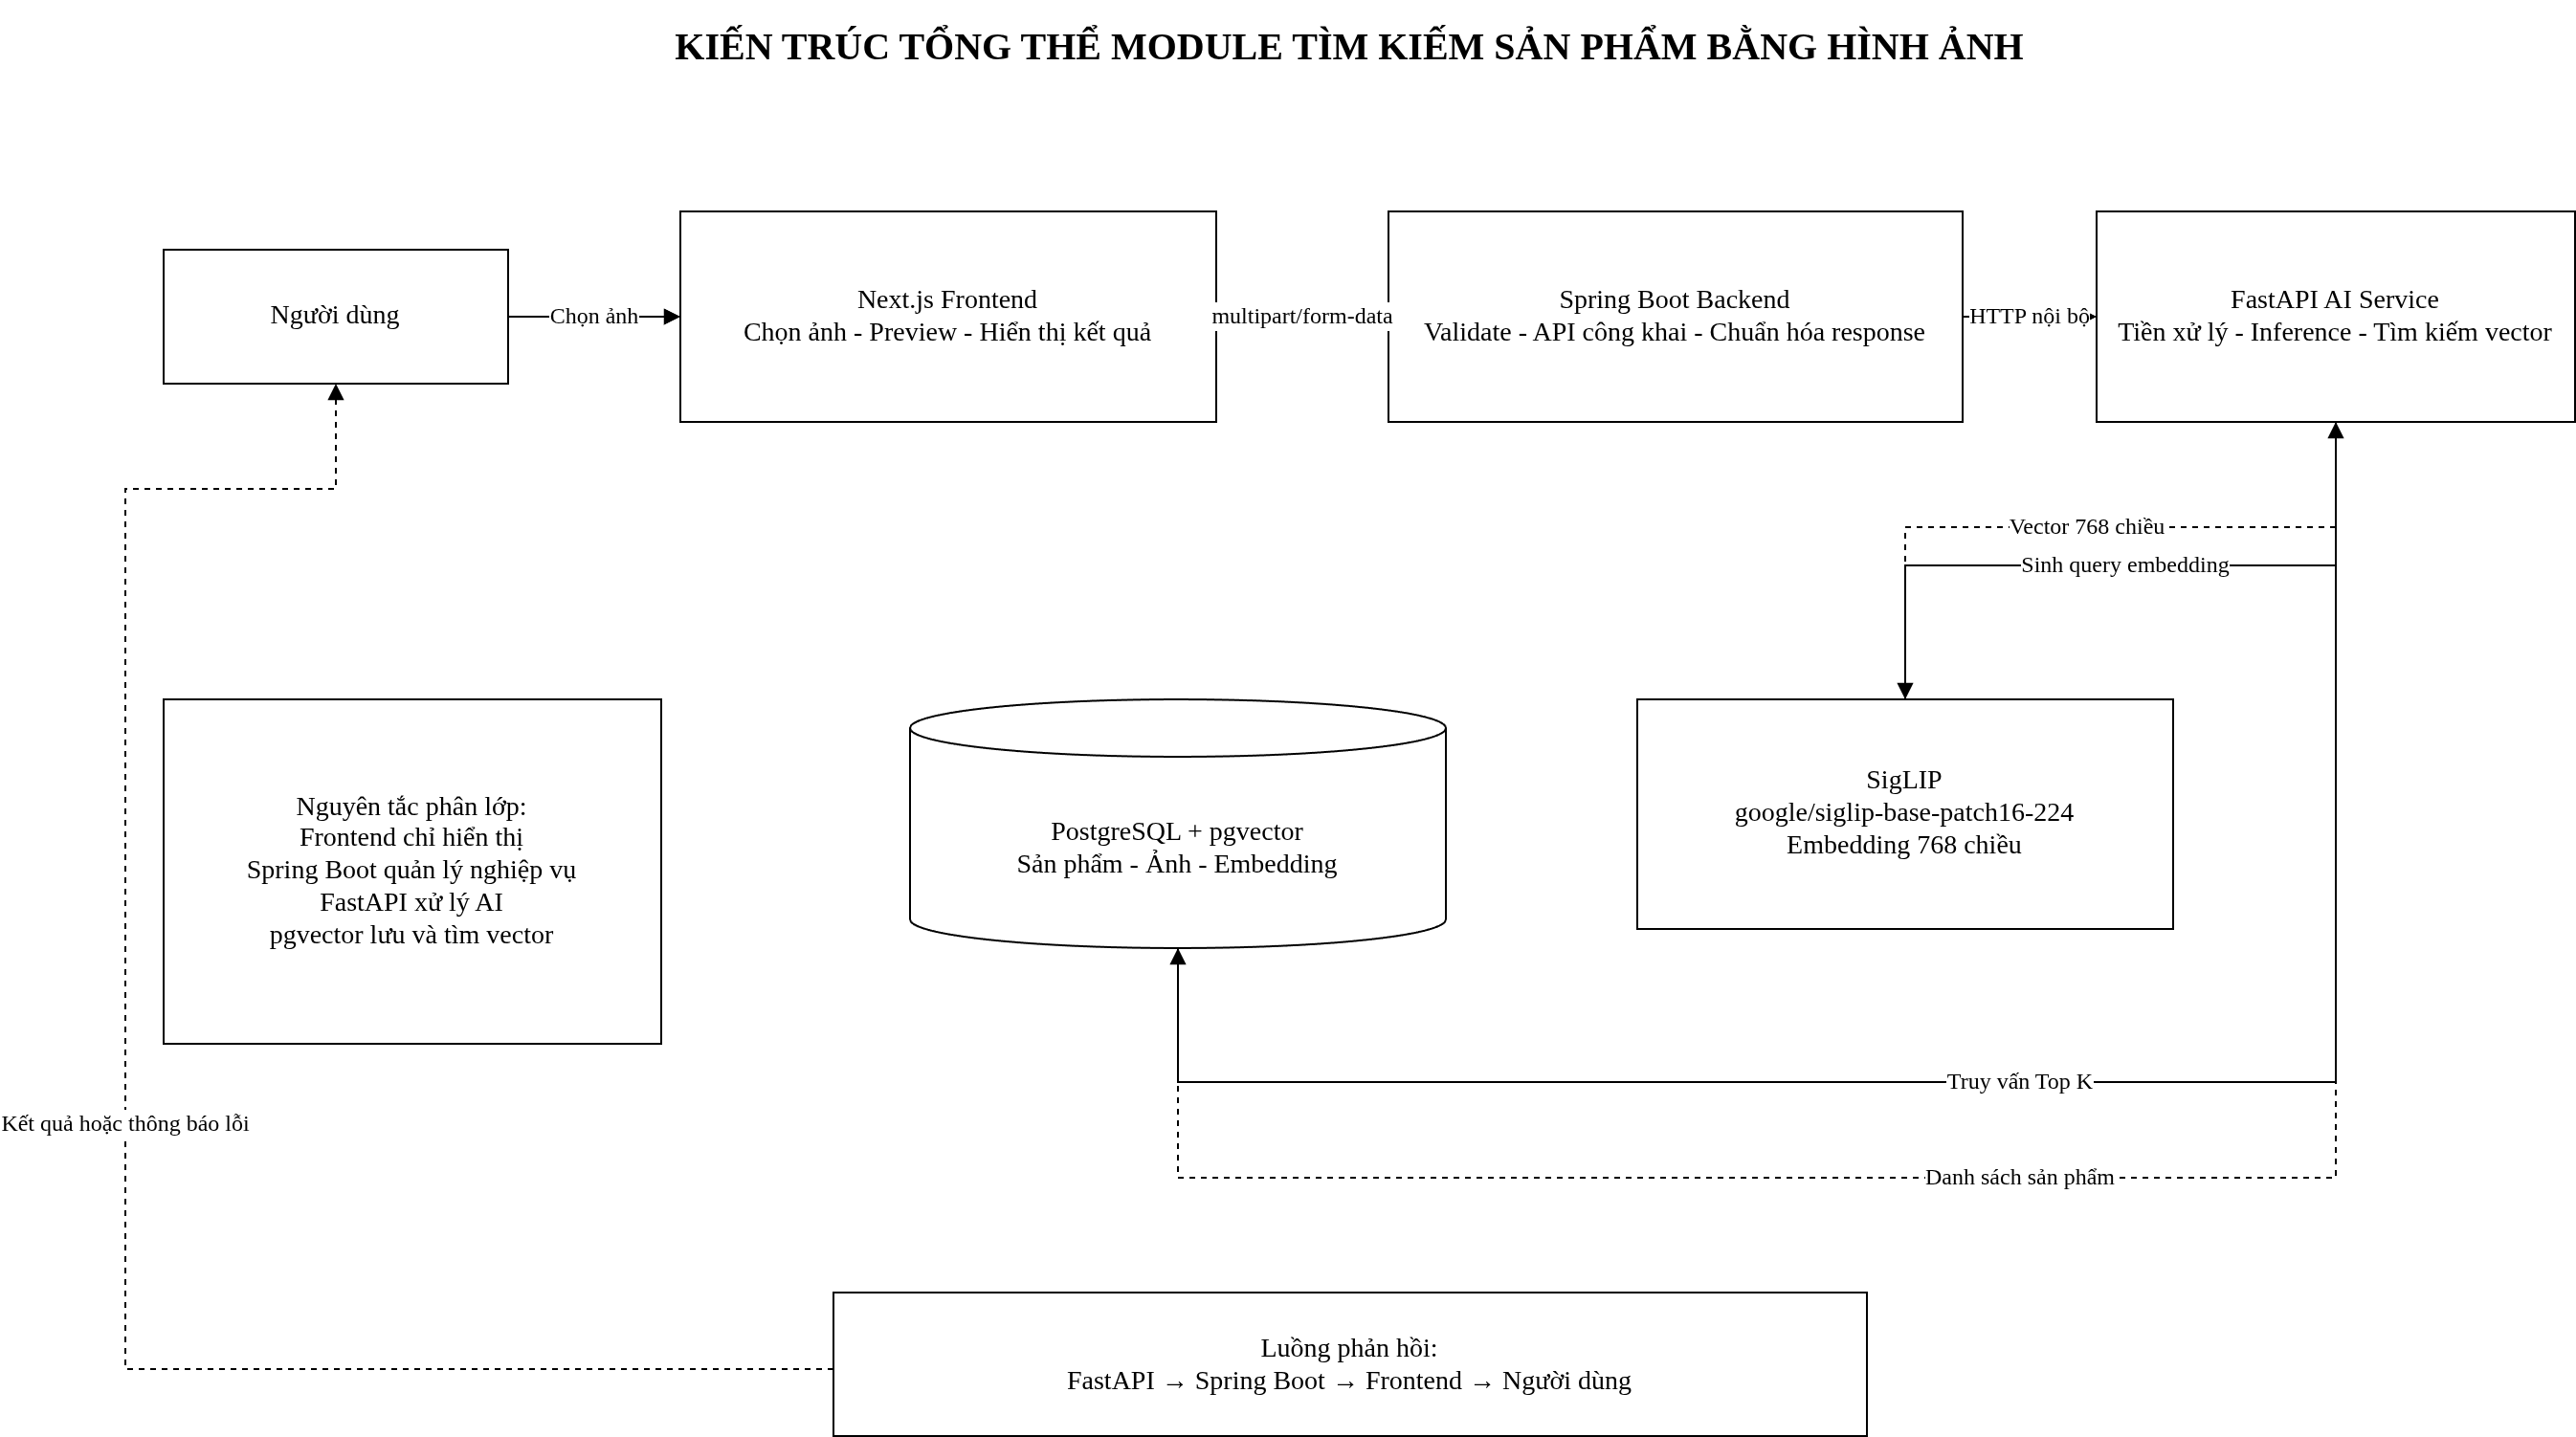
\includegraphics[width=\textwidth]
    {Image/So_do_module_tim_kiem_san_pham_bang_hinh_anh-1. Kiến trúc tổng thể.drawio.png}
    \caption{Sơ đồ kiến trúc module tìm kiếm bằng hình ảnh}
    \label{fig:image-search-architecture}
\end{figure}


\subsubsection{Sơ đồ tuần tự}
Sơ đồ mô tả quá trình tìm kiếm sản phẩm
dựa trên hình ảnh do người dùng cung cấp.
Hệ thống kiểm tra ảnh đầu vào và chuyển
yêu cầu đến dịch vụ AI. Mô hình SigLIP
trích xuất vector đặc trưng 768 chiều,
sau đó vector được chuẩn hóa L2.
Hệ thống thực hiện tìm kiếm tương đồng
cosine trong PostgreSQL/pgvector và trả về
danh sách sản phẩm phù hợp.
\begin{figure}[H]
    \centering
    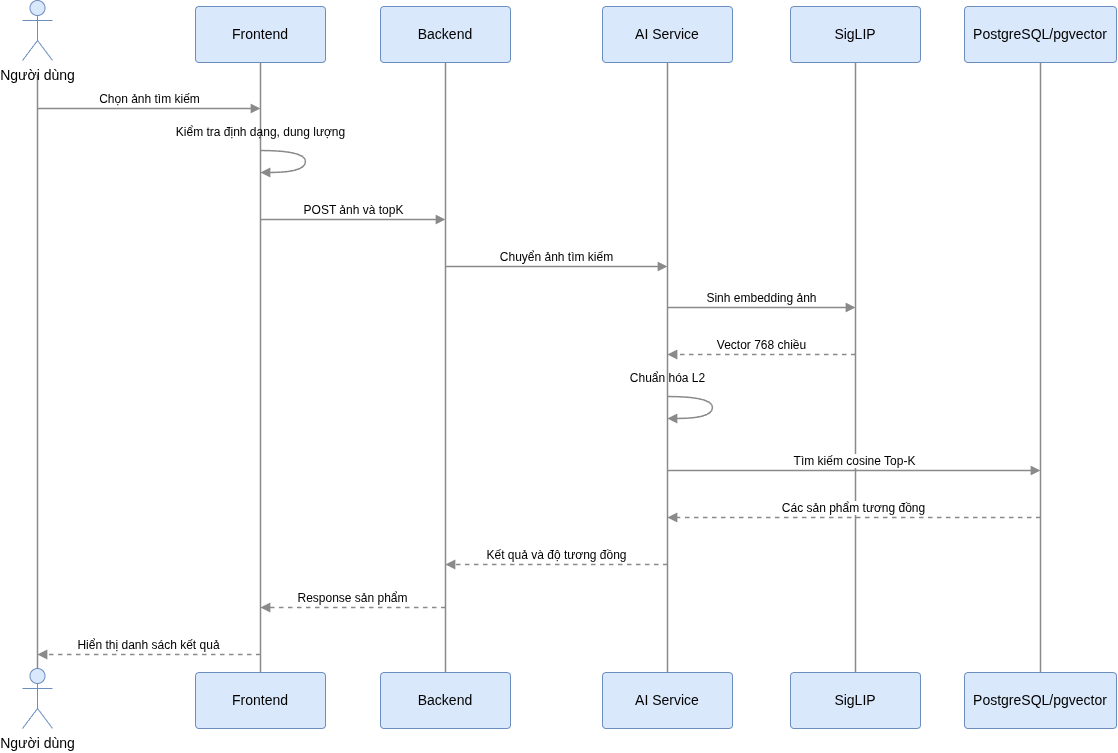
\includegraphics[width=\textwidth]
    {Image/Sequence_TimKiemBangAnh.drawio.png}
    \caption{Sơ đồ tuần tự module tìm kiếm sản phẩm
    bằng hình ảnh}
    \label{fig:sequence-image-search}
\end{figure}


\subsection{Thiết kế module gợi ý sản phẩm cá nhân hóa}
Module gợi ý sản phẩm được thiết kế nhằm đề xuất
những sản phẩm phù hợp với sở thích và hành vi
mua sắm của người dùng.

\subsubsection{Sơ đồ Use Case}
Sơ đồ Use Case thể hiện các chức năng chính
của module đối với người dùng và quản trị viên.\\\\
Người dùng có thể xem danh sách sản phẩm gợi ý
và truy cập thông tin chi tiết sản phẩm.
Các hành vi tương tác được hệ thống ghi nhận
để phục vụ quá trình cá nhân hóa.\\\\
Quản trị viên thực hiện quản lý dữ liệu tương tác,
hồ sơ sở thích và dữ liệu phục vụ gợi ý sản phẩm.
\begin{figure}[H]
    \centering
    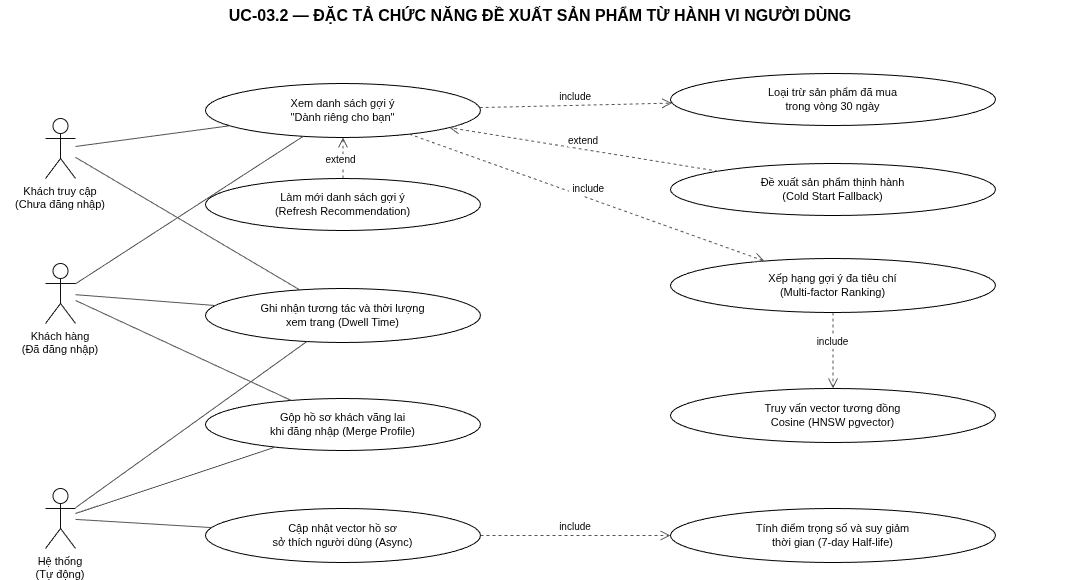
\includegraphics[width=\textwidth]
    {Image/UC-03.2_De_xuat_san_pham_tu_hanh_vi-UC-03.2_De_Xuat_Hanh_Vi.drawio.png}
    \caption{Sơ đồ Use Case module gợi ý sản phẩm cá nhân hóa}
    \label{fig:recommendation-usecase}
\end{figure}

\subsubsection{Sơ đồ kiến trúc}
Module gợi ý sử dụng dữ liệu sản phẩm,
lịch sử tương tác và hồ sơ sở thích người dùng.\\\\
Các hành vi như xem sản phẩm, thêm vào danh sách
yêu thích, thêm vào giỏ hàng và đặt hàng
được ghi nhận để xác định mức độ quan tâm
của người dùng đối với sản phẩm.\\\\
Dựa trên dữ liệu thu thập, hệ thống xây dựng
hồ sơ sở thích, lựa chọn các sản phẩm ứng viên
và đánh giá mức độ phù hợp để tạo danh sách gợi ý.
\begin{figure}[H]
    \centering
    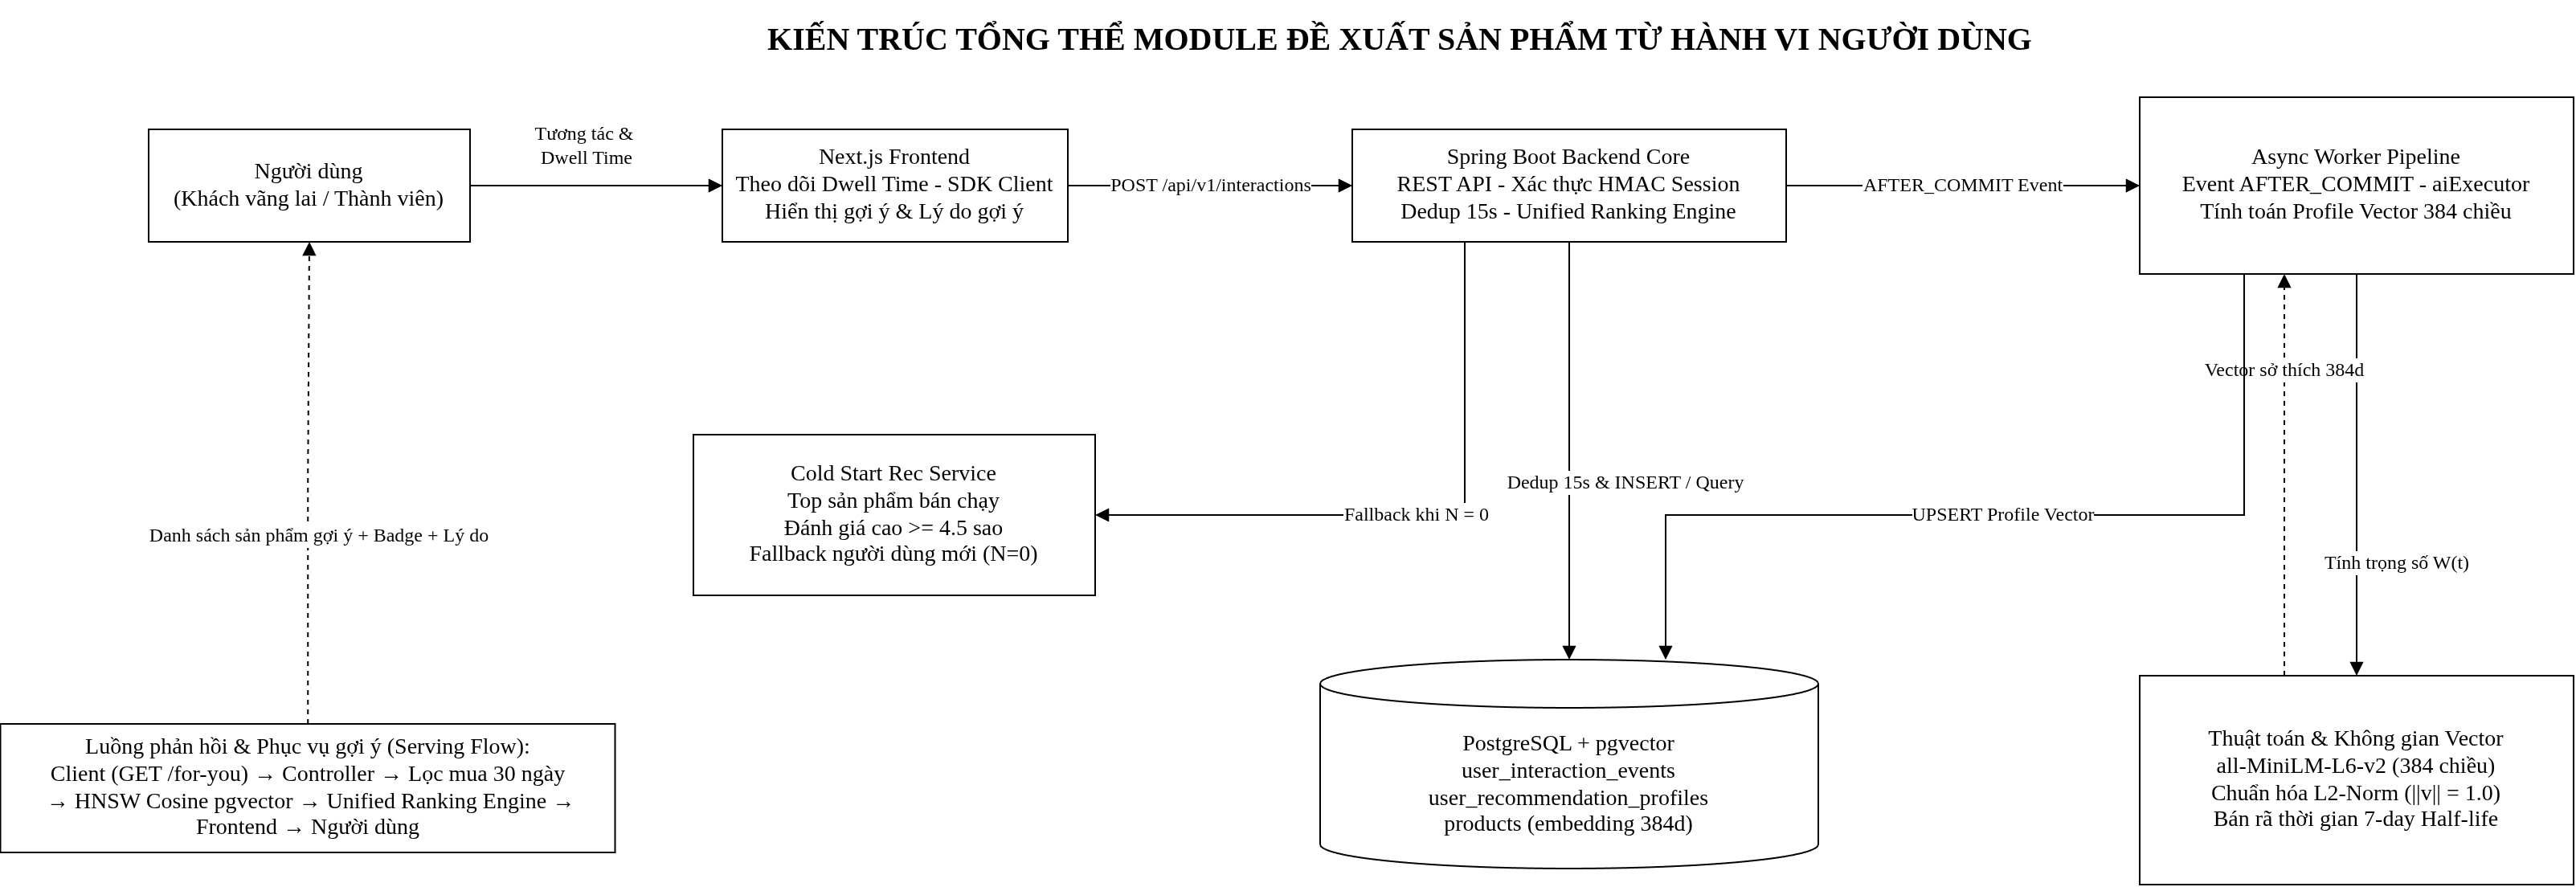
\includegraphics[width=\textwidth]
    {Image/So_do_module_de_xuat_san_pham_tu_hanh_vi.drawio.png}
    \caption{Sơ đồ kiến trúc module gợi ý sản phẩm cá nhân hóa}
    \label{fig:recommendation-architecture}
\end{figure}

\subsubsection{Sơ đồ tuần tự}
Sơ đồ tuần tự mô tả quá trình ghi nhận
hành vi người dùng và tạo danh sách
sản phẩm gợi ý. Hệ thống thu thập
các tương tác như xem sản phẩm,
thời gian xem và đánh dấu yêu thích.
Dữ liệu được xử lý để cập nhật hồ sơ
sở thích của người dùng.\\\\
Khi người dùng truy cập trang chủ,
hệ thống phân tích hồ sơ sở thích,
truy xuất các sản phẩm tiềm năng
và xếp hạng theo mức độ phù hợp
trước khi hiển thị danh sách gợi ý.
\begin{figure}[H]
    \centering
    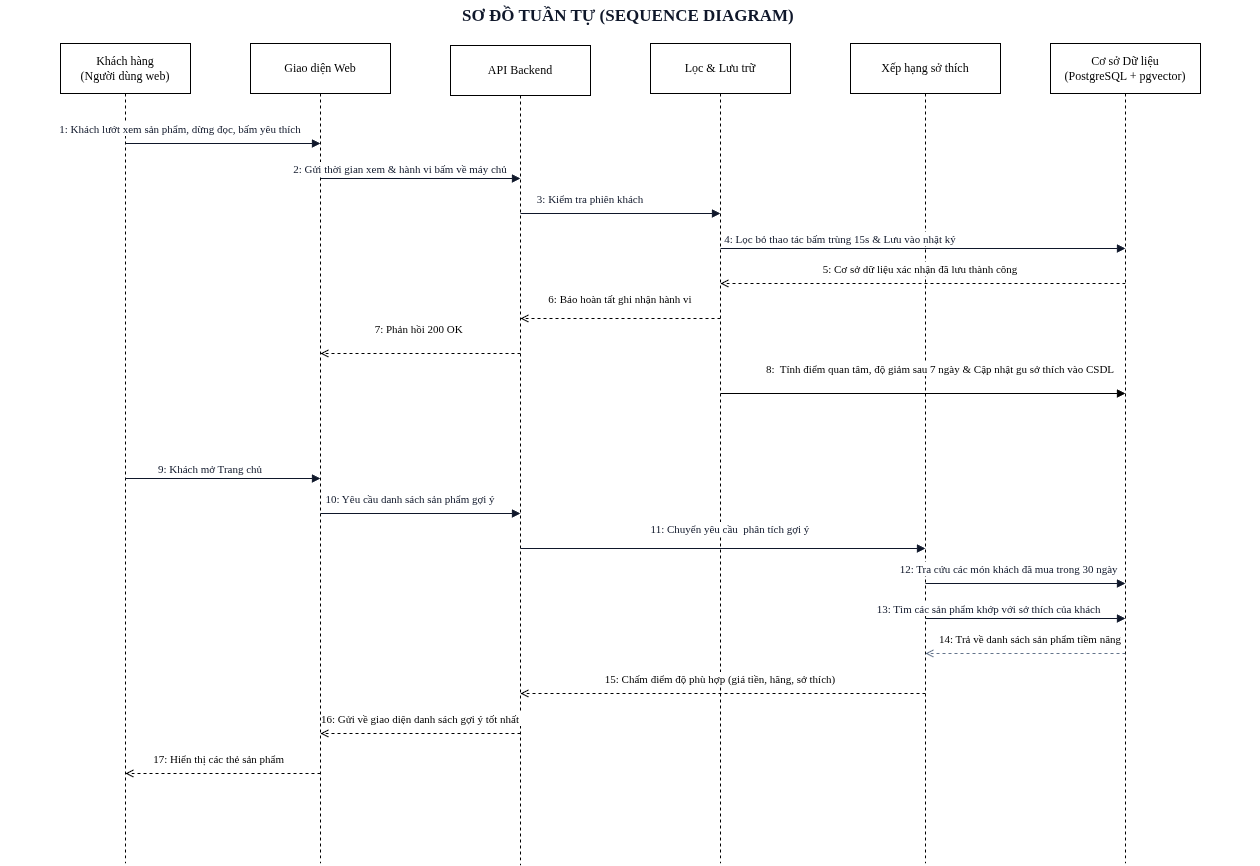
\includegraphics[width=\textwidth]
    {Image/sơ đồ tuần tự gợi ý sản phẩm từ hành vi người dùng.drawio.png}
    \caption{Sơ đồ tuần tự module gợi ý sản phẩm
    dựa trên hành vi người dùng}
    \label{fig:sequence-recommendation}
\end{figure}

\chapter{TRIỂN KHAI VÀ KIỂM THỬ HỆ THỐNG}
\section{Môi trường và công nghệ triển khai}

\subsection{Môi trường triển khai}

Hệ thống TechWiseAI được phát triển và triển khai
thử nghiệm trên hệ điều hành Windows. Các thành phần
Frontend, Backend, dịch vụ trí tuệ nhân tạo và
cơ sở dữ liệu được cấu hình để hoạt động trong
môi trường phát triển cục bộ.

\subsection{Các công nghệ sử dụng}

\subsubsection{Next.js}

Next.js là framework phát triển ứng dụng web
dựa trên React, hỗ trợ xây dựng giao diện
và tối ưu hiệu năng hiển thị. Trong hệ thống
TechWiseAI, Next.js được sử dụng để phát triển
giao diện người dùng, trang quản trị và tích hợp
các chức năng trí tuệ nhân tạo.

\subsubsection{Spring Boot}

Spring Boot là framework phát triển ứng dụng
Java, hỗ trợ xây dựng các dịch vụ RESTful API.
Trong hệ thống, Spring Boot đảm nhiệm xử lý
nghiệp vụ thương mại điện tử, xác thực,
phân quyền và kết nối cơ sở dữ liệu,
đồng thời đóng vai trò trung gian
giữa Frontend và các dịch vụ AI.

\subsubsection{Python và FastAPI}

Python được sử dụng để phát triển các chức năng
trí tuệ nhân tạo. FastAPI là framework hỗ trợ
xây dựng API với hiệu năng cao và khả năng
xử lý bất đồng bộ. Trong TechWiseAI,
FastAPI được sử dụng để triển khai
các dịch vụ xử lý và suy luận AI.

\subsubsection{PostgreSQL và pgvector}

PostgreSQL là hệ quản trị cơ sở dữ liệu
quan hệ mã nguồn mở, được sử dụng để
lưu trữ dữ liệu của hệ thống.
Phần mở rộng pgvector hỗ trợ lưu trữ
và tìm kiếm vector, phục vụ các chức năng
tìm kiếm ngữ nghĩa và tìm kiếm bằng hình ảnh.

\subsubsection{BAAI/bge-m3}

BAAI/bge-m3 là mô hình embedding đa ngôn ngữ,
được sử dụng để chuyển đổi nội dung văn bản
thành vector biểu diễn ngữ nghĩa.
Trong module chatbot RAG, mô hình hỗ trợ
biểu diễn thông tin sản phẩm và truy vấn
của người dùng để thực hiện tìm kiếm tương đồng.

\subsubsection{SigLIP}

SigLIP là mô hình học biểu diễn đa phương thức,
có khả năng trích xuất đặc trưng từ hình ảnh
và văn bản. Trong hệ thống, SigLIP được sử dụng
để tạo vector đặc trưng hình ảnh,
phục vụ chức năng tìm kiếm sản phẩm
dựa trên mức độ tương đồng.

\subsubsection{Mô hình ngôn ngữ lớn}

Mô hình ngôn ngữ lớn được sử dụng trong
module chatbot RAG để tổng hợp thông tin
truy xuất và sinh câu trả lời tư vấn.
Nội dung phản hồi được xây dựng dựa trên
ngữ cảnh sản phẩm do hệ thống cung cấp,
nhằm hạn chế thông tin không có trong dữ liệu.

\subsubsection{Git}

Git là hệ thống quản lý phiên bản phân tán,
được sử dụng để theo dõi thay đổi mã nguồn,
quản lý các nhánh phát triển và hỗ trợ
quá trình làm việc nhóm.

\section{Triển khai hệ thống thương mại điện tử}
Hệ thống thương mại điện tử TechWiseAI được
triển khai theo kiến trúc phân tách giữa
Frontend và Backend. Giao diện được xây dựng
bằng Next.js, trong khi Spring Boot đảm nhiệm
xử lý nghiệp vụ và cung cấp các REST API.
Dữ liệu được lưu trữ trong PostgreSQL.

\subsection{Triển khai chức năng tài khoản}
Hệ thống hỗ trợ đăng ký, đăng nhập, quản lý
thông tin cá nhân và phân quyền người dùng.
Các yêu cầu từ giao diện được gửi đến Backend
để xác thực, xử lý và trả về kết quả tương ứng.

\begin{figure}[H]
    \centering
    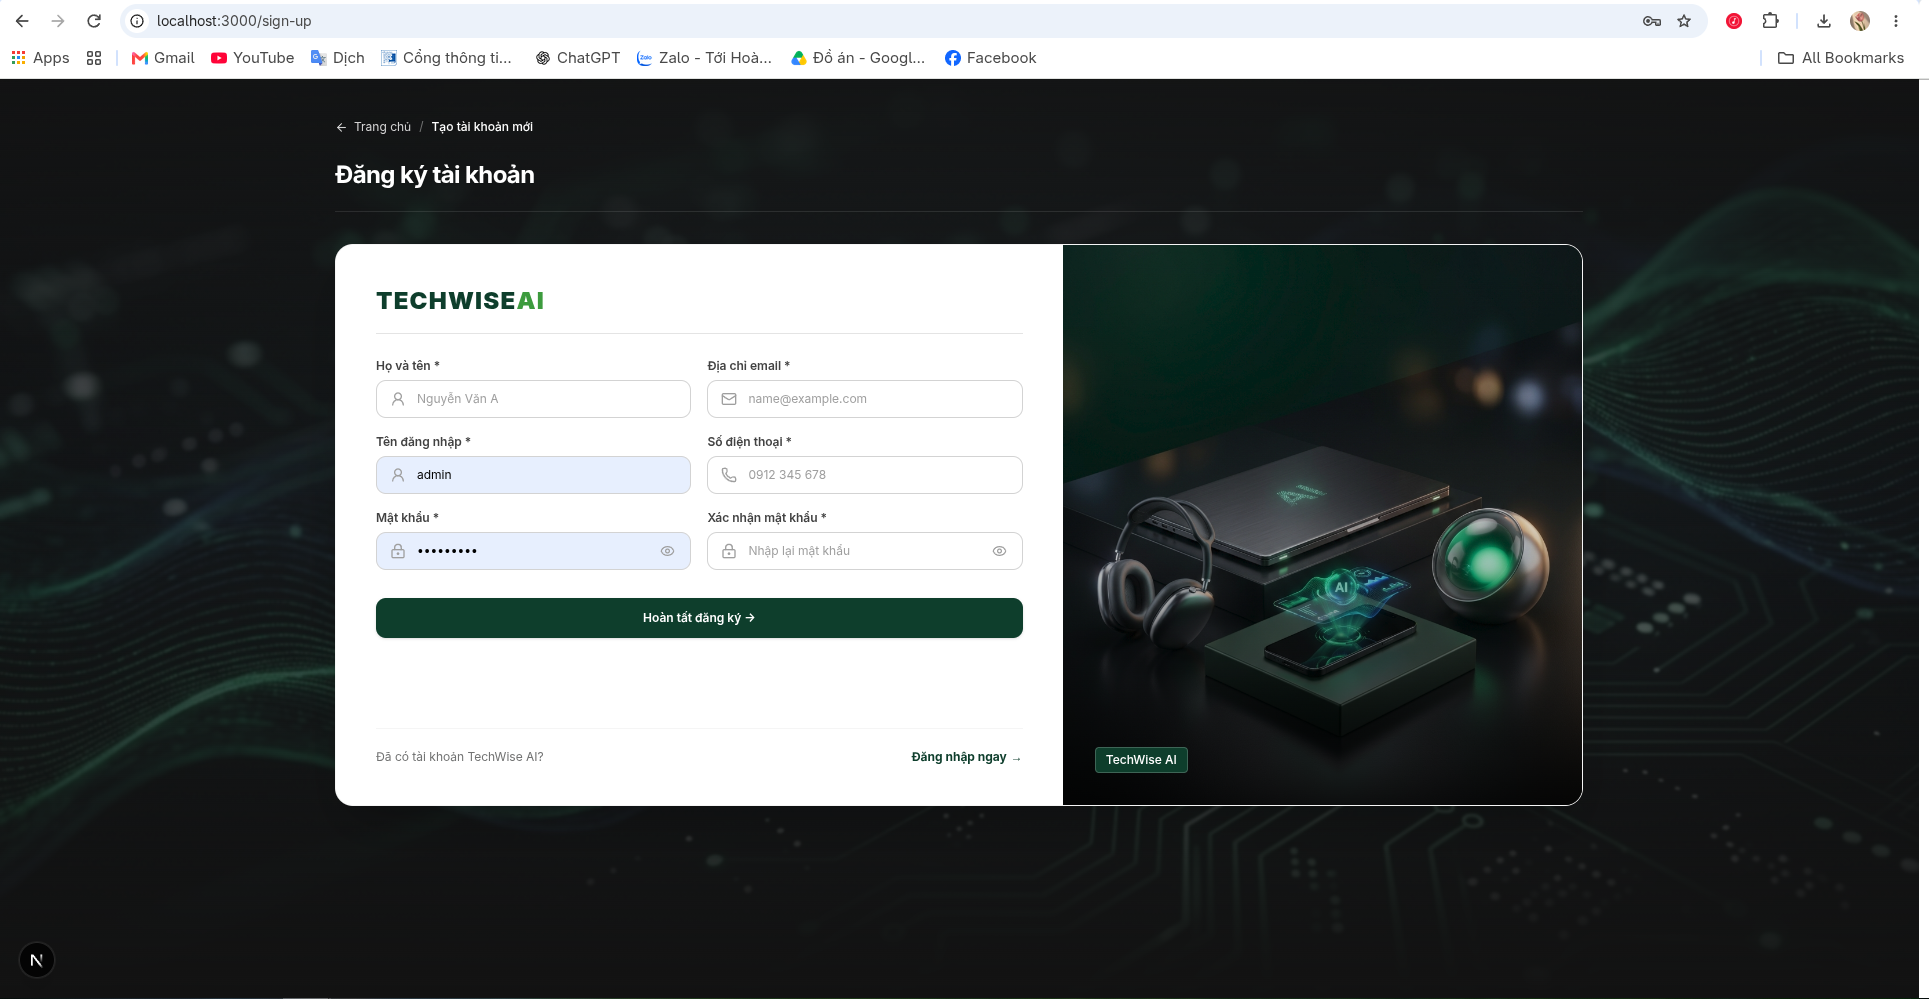
\includegraphics[width=\textwidth]
    {Image/dangky.png}
    \caption{Giao diện đăng ký tài khoản}
    \label{fig:signup-form}
\end{figure}
\begin{figure}[H]
    \centering
    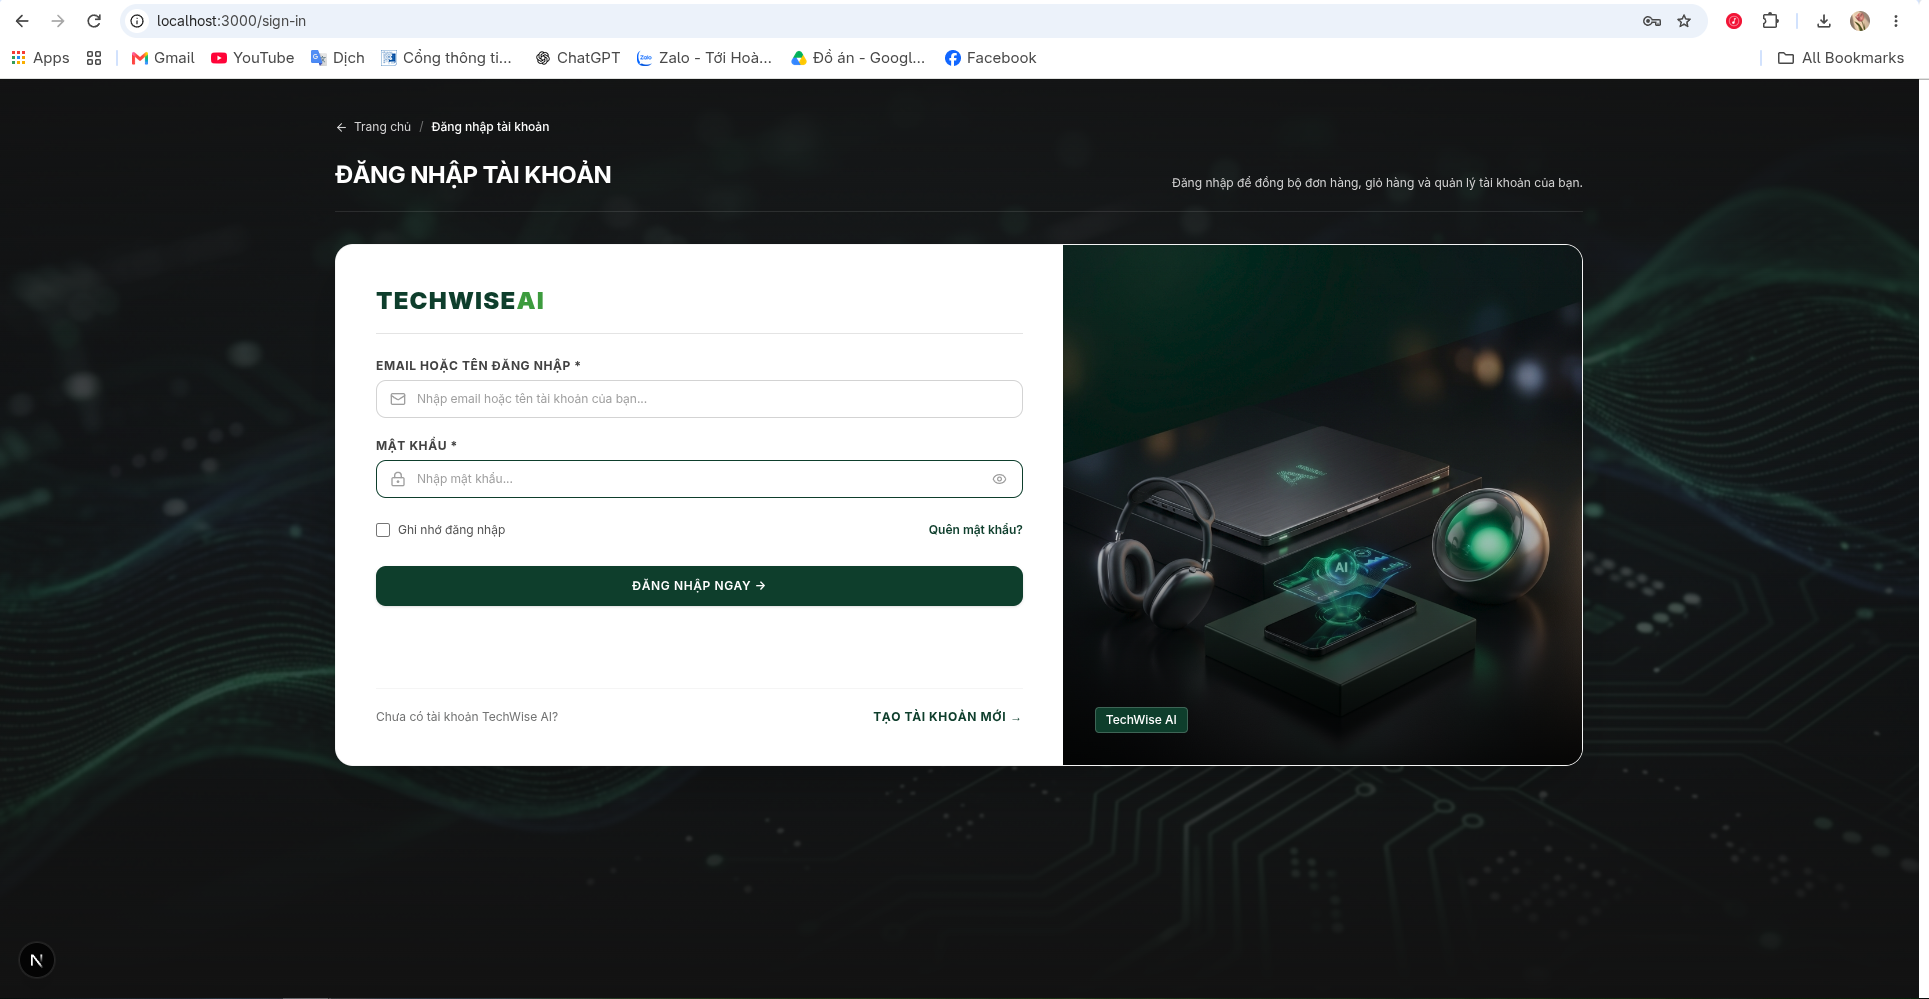
\includegraphics[width=\textwidth]
    {Image/danhnhap.png}
    \caption{Giao diện đăng nhập tài khoản}
    \label{fig:login-form}
\end{figure}

\subsection{Triển khai chức năng sản phẩm}

Chức năng sản phẩm cho phép người dùng xem
danh sách, tìm kiếm, lọc và xem thông tin
chi tiết sản phẩm. Quản trị viên có thể
thêm mới, chỉnh sửa và quản lý sản phẩm
thông qua giao diện quản trị.
\begin{figure}[H]
    \centering
    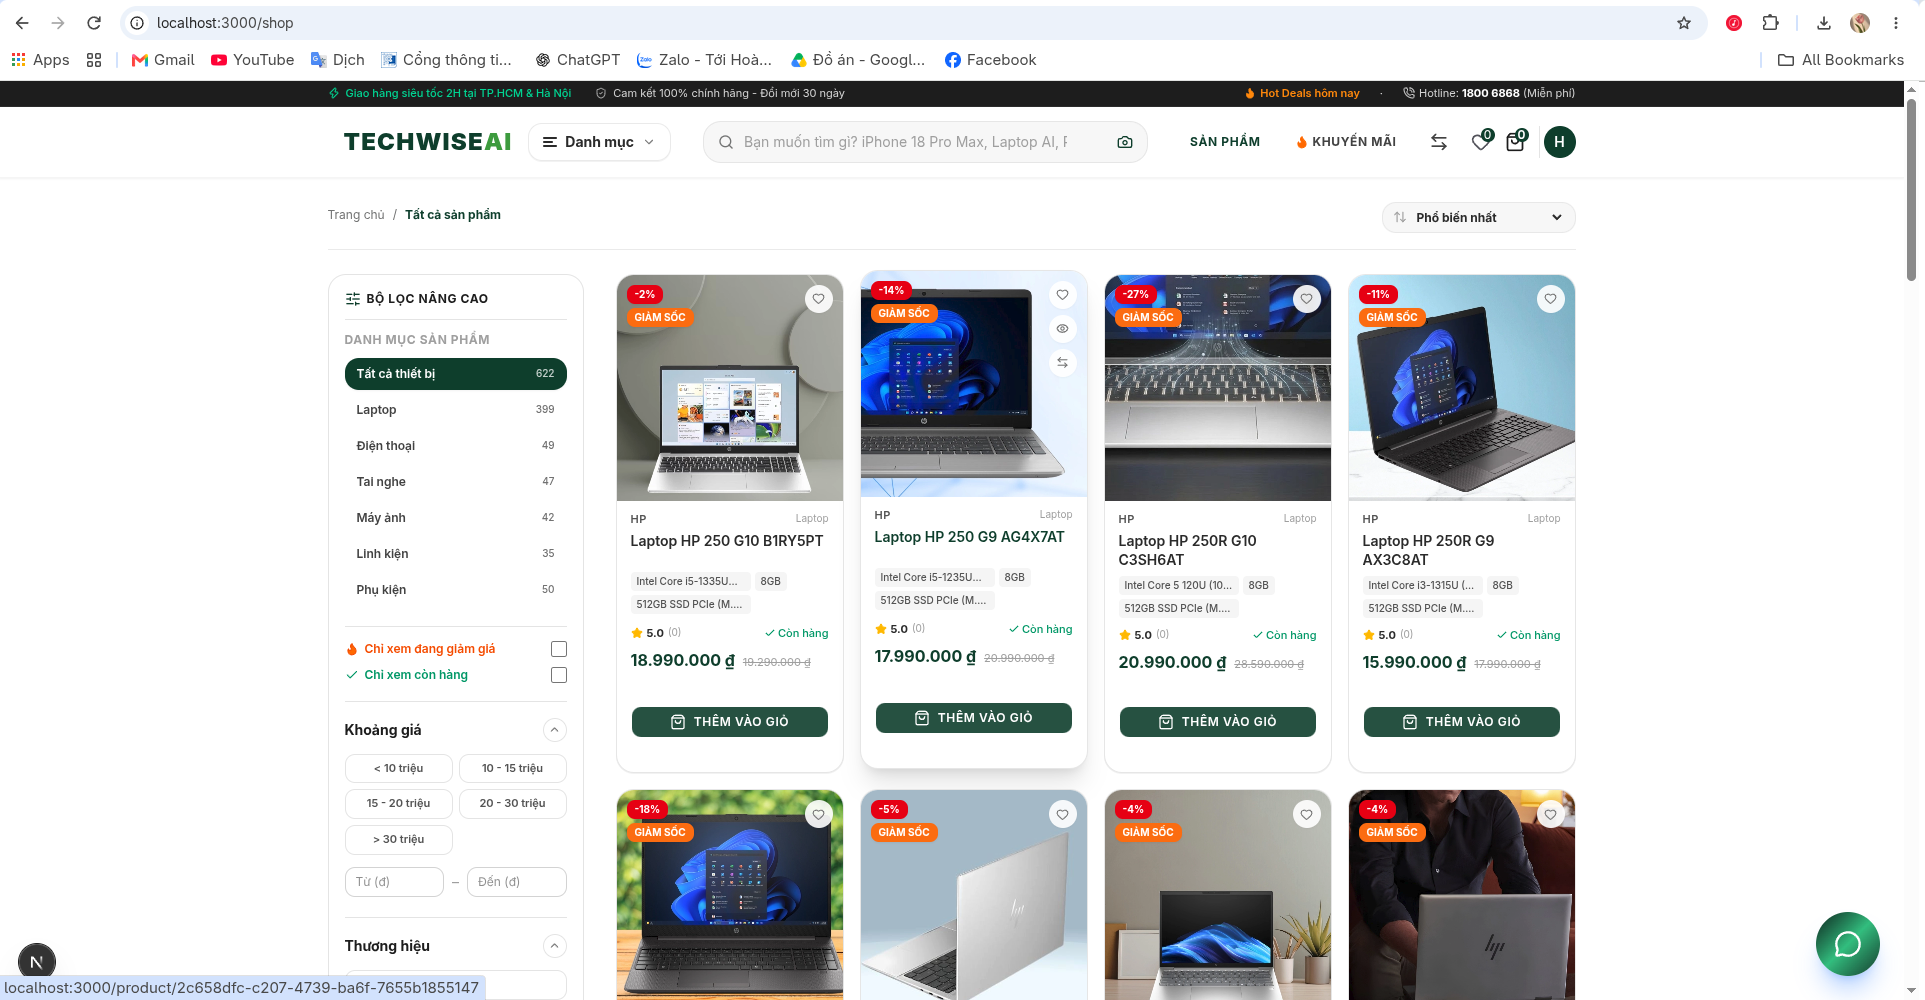
\includegraphics[width=\textwidth]
    {Image/danhsach.png}
    \caption{Giao diện danh sách sản phẩm}
    \label{fig:products-list}
\end{figure}
\begin{figure}[H]
    \centering
    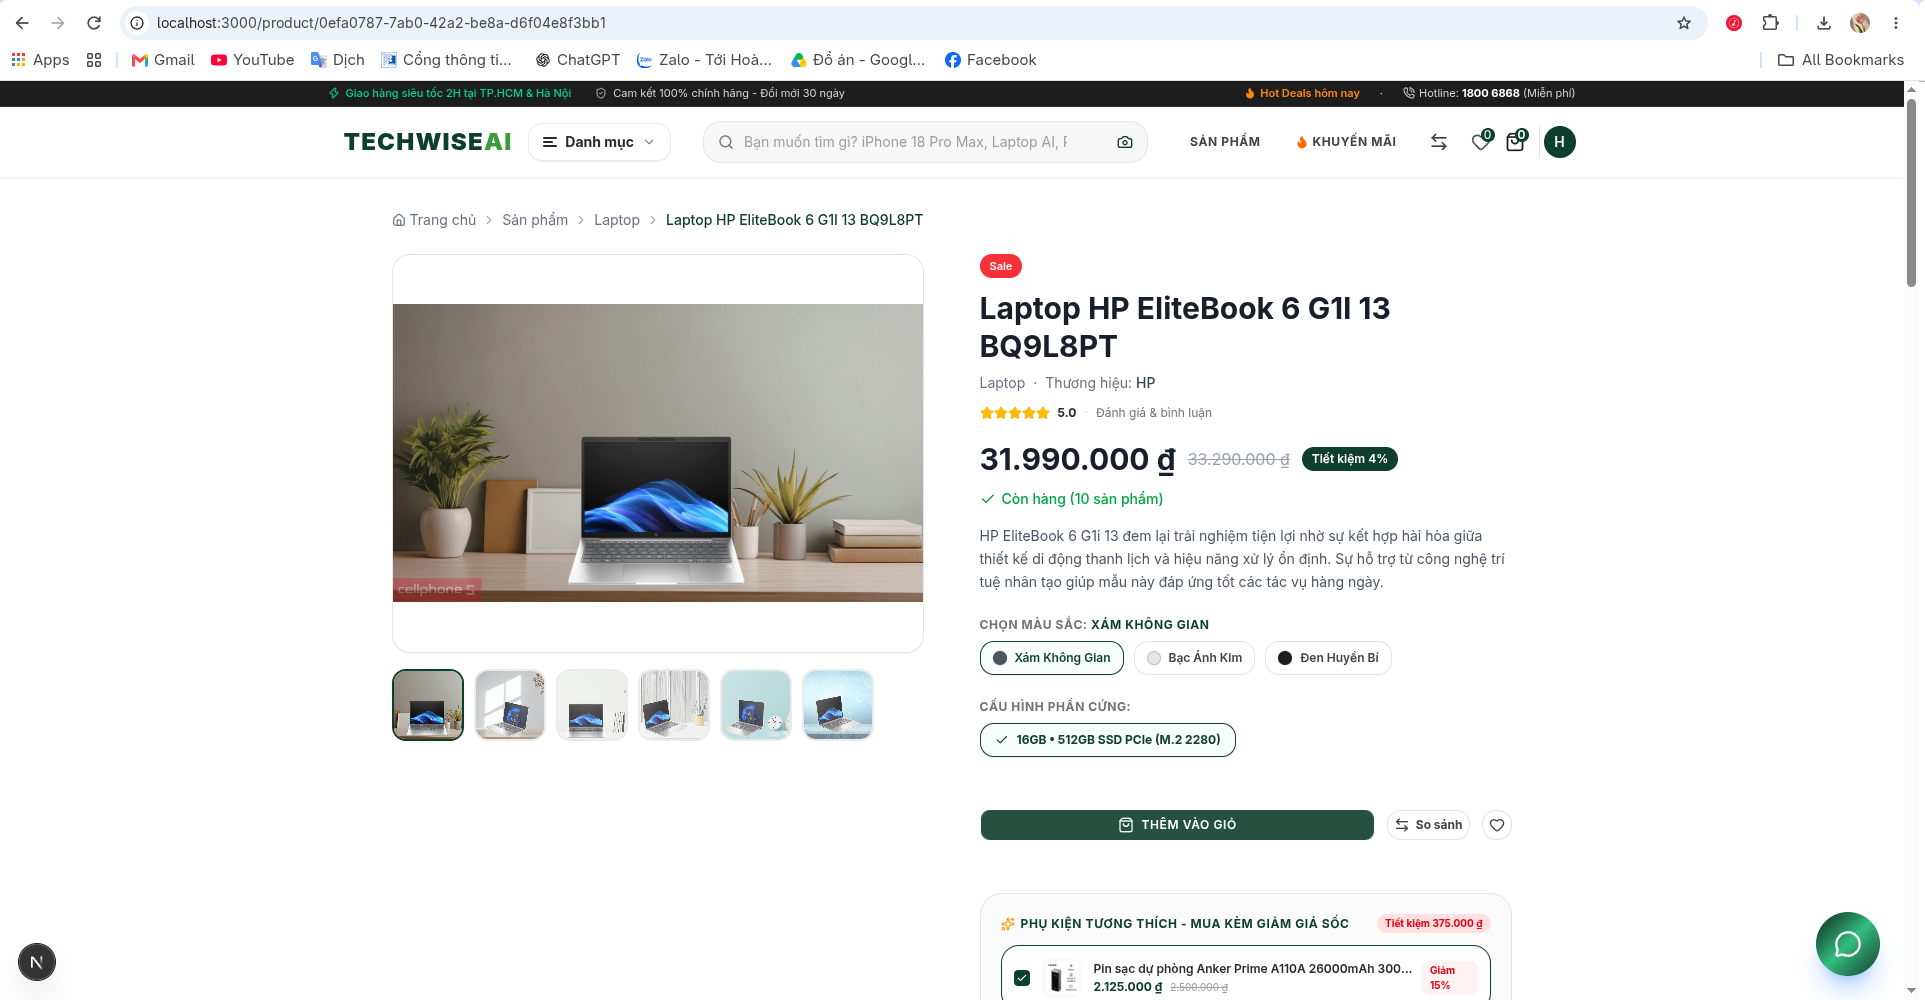
\includegraphics[width=\textwidth]
    {Image/chitiet.png}
    \caption{Giao diện thông tin sản phẩm chi tiết}
    \label{fig:products-view}
\end{figure}
\begin{figure}[H]
    \centering
    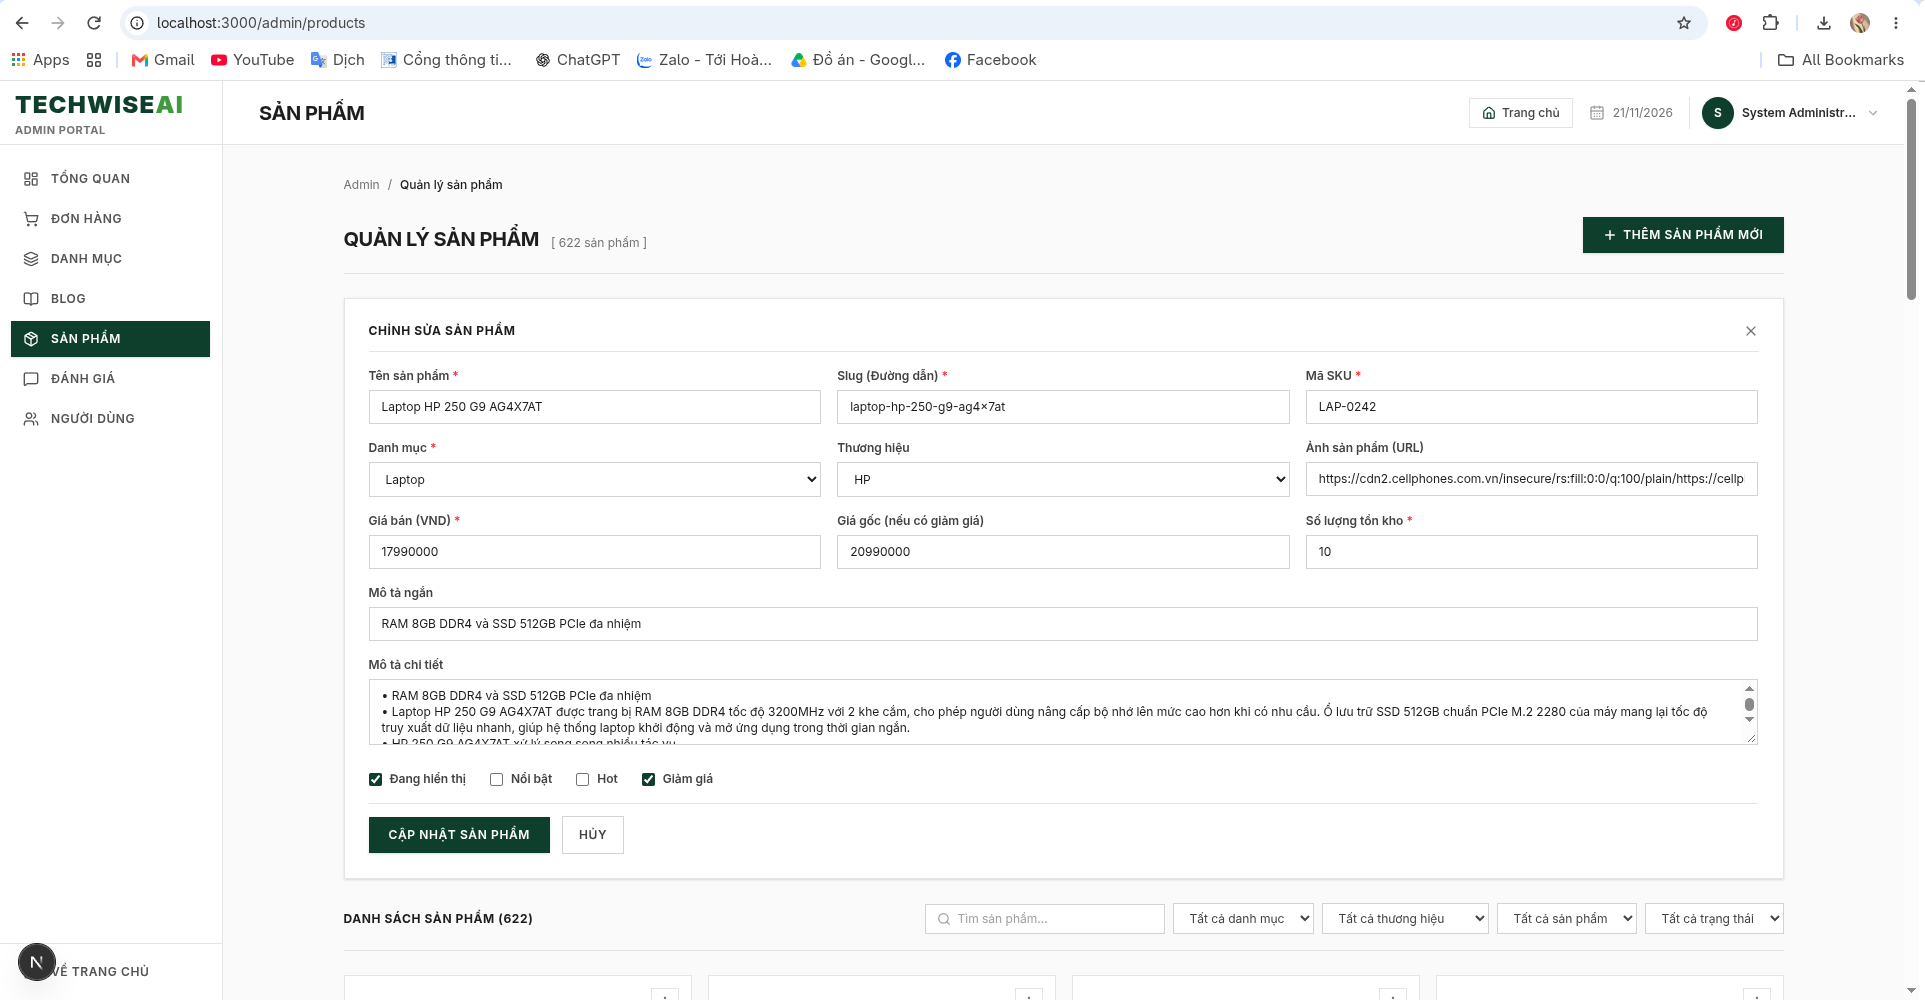
\includegraphics[width=\textwidth]
    {Image/quanly.png}
    \caption{Giao diện quản lý sản phẩm}
    \label{fig:products}
\end{figure}

\subsection{Triển khai chức năng giỏ hàng và đặt hàng}
Người dùng có thể thêm sản phẩm vào giỏ hàng,
thay đổi số lượng và tiến hành đặt hàng.
Backend tiếp nhận yêu cầu, xử lý thông tin
và lưu trữ dữ liệu đơn hàng trong cơ sở dữ liệu.
\begin{figure}[H]
    \centering
    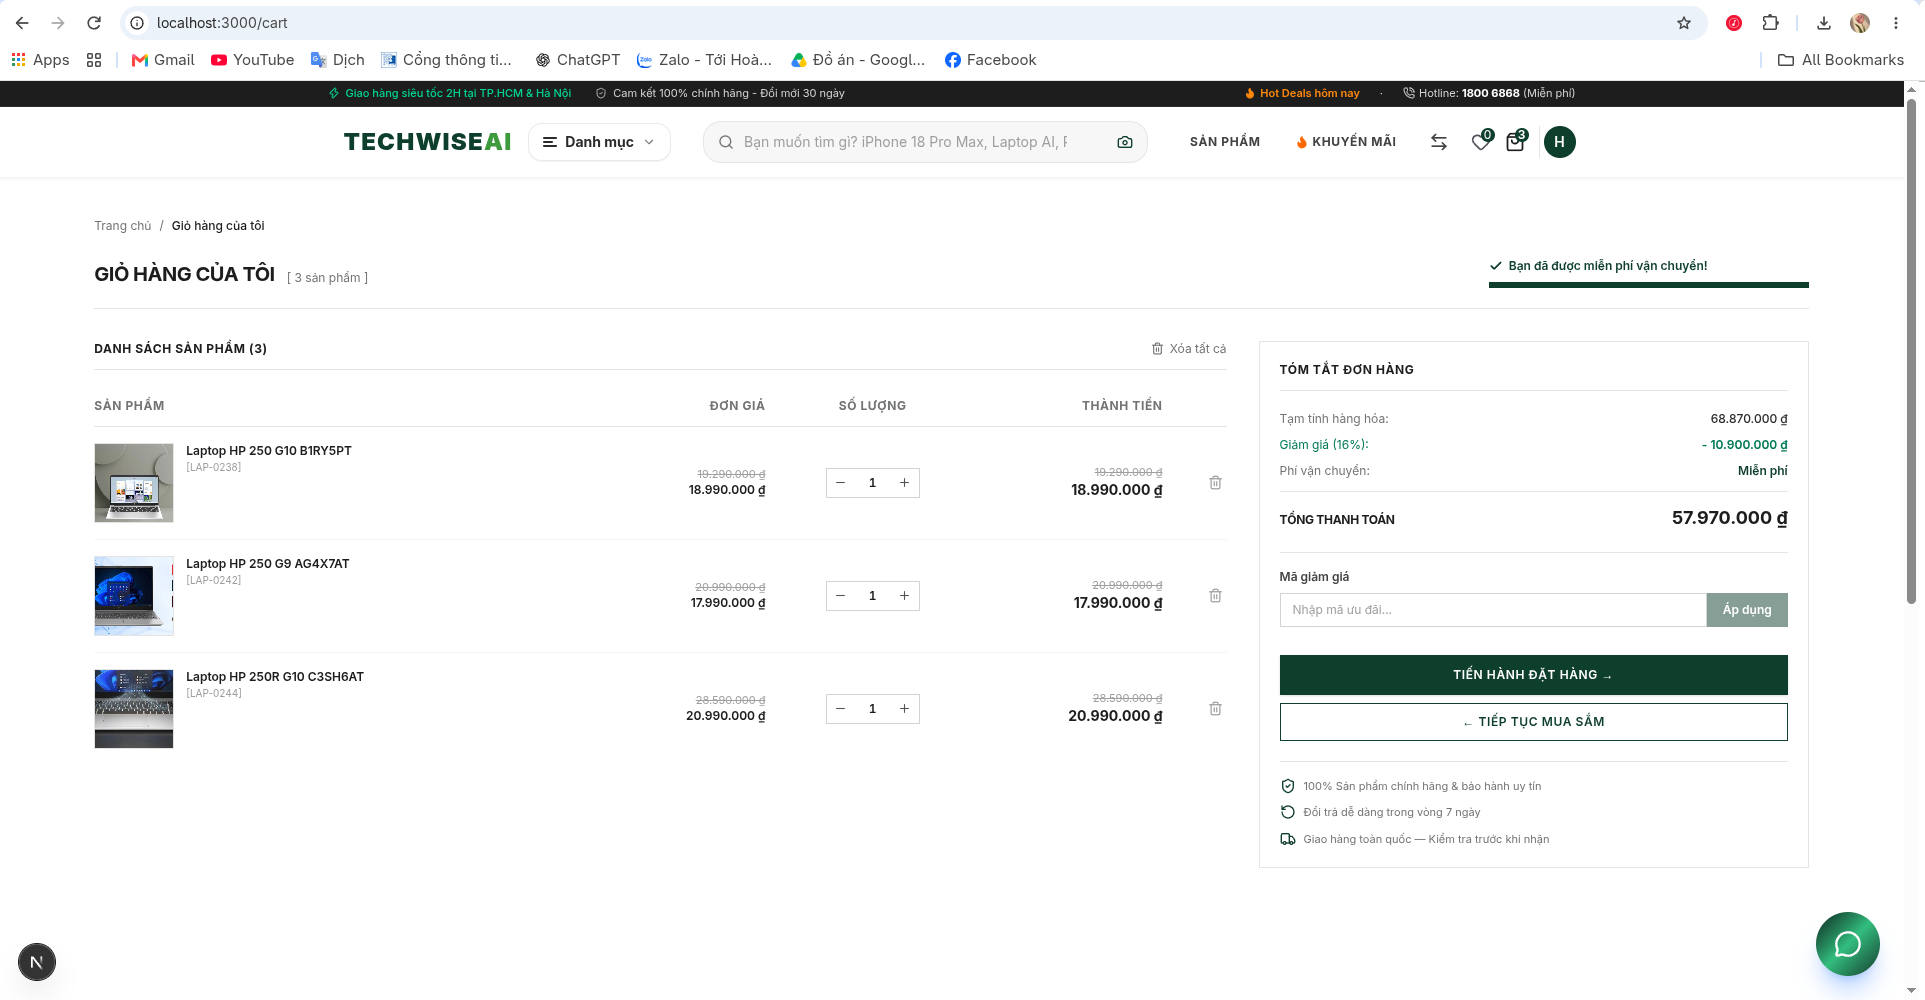
\includegraphics[width=\textwidth]
    {Image/giohang.png}
    \caption{Giao diện giỏ hàng}
    \label{fig:products}
\end{figure}
\begin{figure}[H]
    \centering
    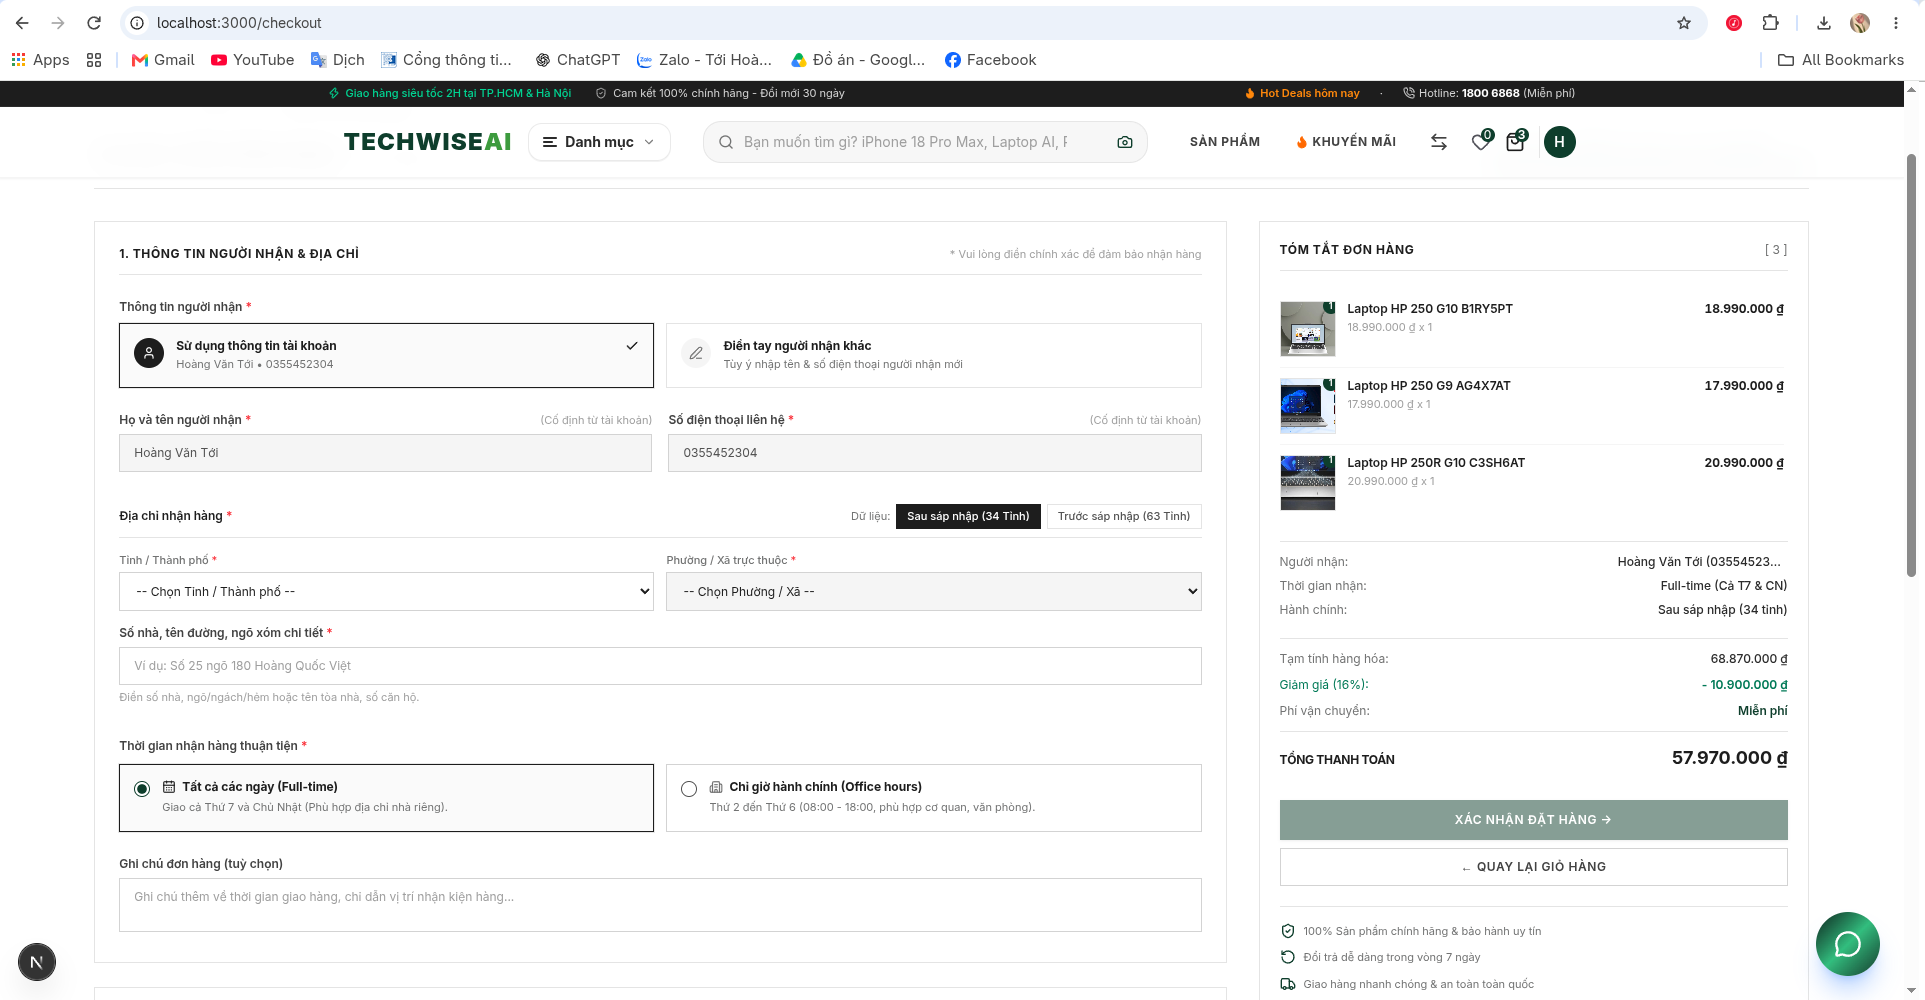
\includegraphics[width=\textwidth]
    {Image/dathang.png}
    \caption{Giao diện đặt hàng}
    \label{fig:products}
\end{figure}

\subsection{Triển khai các chức năng hỗ trợ}

Ngoài các chức năng chính, hệ thống còn hỗ trợ
đánh giá sản phẩm, quản lý danh sách yêu thích,
khôi phục mật khẩu và hiển thị bài viết.
Các chức năng này góp phần hoàn thiện
trải nghiệm mua sắm của người dùng.
\begin{figure}[H]
    \centering
    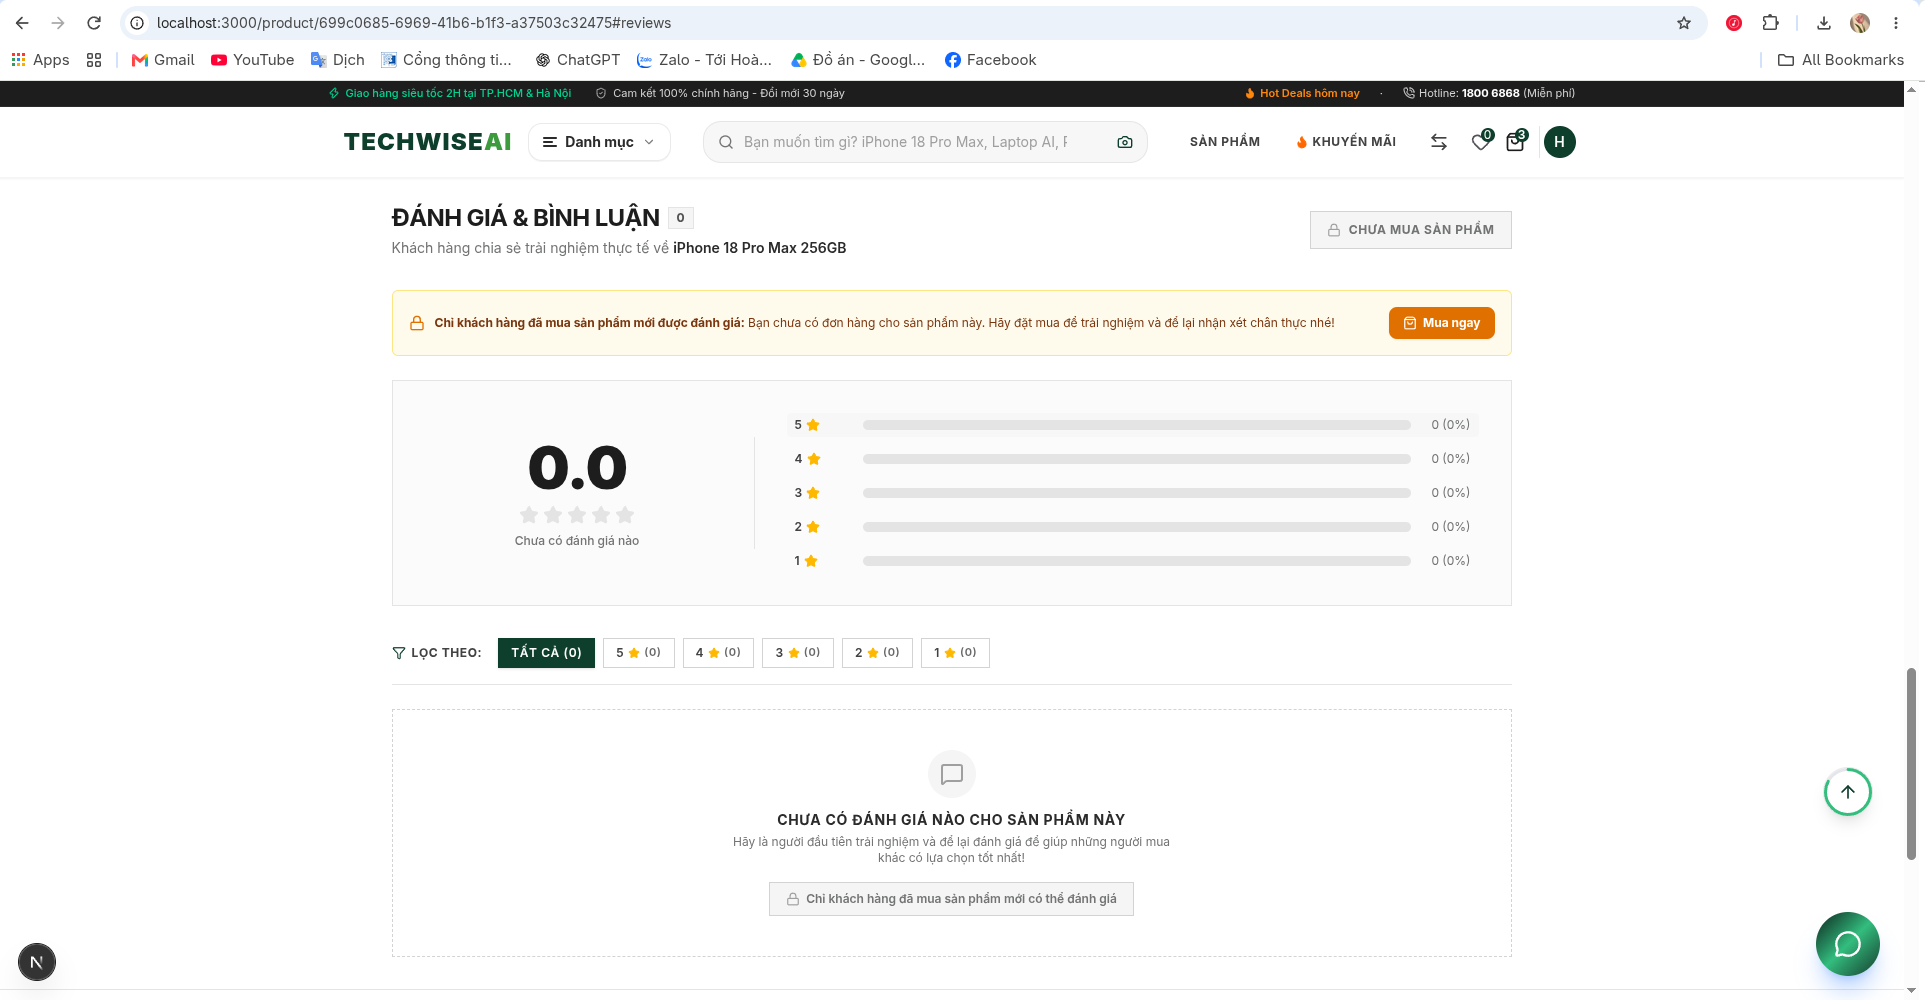
\includegraphics[width=\textwidth]
    {Image/danhgia.png}
    \caption{Giao diện đánh giá sản phẩm}
    \label{fig:rewview}
\end{figure}

\section{Kiểm thử và đánh giá hệ thống}

\subsection{Kiểm thử các chức năng nghiệp vụ}

Các chức năng được kiểm thử nhằm xác định
khả năng xử lý yêu cầu và tính chính xác
của kết quả trả về.

\begin{table}[htbp]
    \centering
    \caption{Kiểm thử các chức năng nghiệp vụ}
    \label{tab:business-testing}
    \renewcommand{\arraystretch}{1.3}
    \begin{tabular}{|p{1cm}|p{4cm}|p{5cm}|p{2cm}|}
        \hline
        \textbf{STT} &
        \textbf{Chức năng} &
        \textbf{Kết quả mong đợi} &
        \textbf{Kết quả} \\
        \hline
        1 & Đăng nhập &
        Xác thực tài khoản hợp lệ & Đạt \\
        \hline
        2 & Tìm kiếm sản phẩm &
        Trả về sản phẩm phù hợp & Đạt \\
        \hline
        3 & Thêm vào giỏ hàng &
        Cập nhật giỏ hàng & Đạt \\
        \hline
        4 & Đặt hàng &
        Tạo đơn hàng thành công & Đạt \\
        \hline
        5 & Quản lý sản phẩm &
        Thêm, sửa, xóa dữ liệu & Đạt \\
        \hline
    \end{tabular}
\end{table}

\subsection{Kiểm thử các chức năng trí tuệ nhân tạo}

Các module AI được kiểm thử bằng những yêu cầu
đầu vào khác nhau nhằm đánh giá khả năng
truy xuất, xử lý và trả về kết quả.

\begin{table}[htbp]
    \centering
    \caption{Kiểm thử các module trí tuệ nhân tạo}
    \label{tab:ai-testing}
    \renewcommand{\arraystretch}{1.3}
    \begin{tabular}{|p{1cm}|p{4cm}|p{5cm}|p{2cm}|}
        \hline
        \textbf{STT} &
        \textbf{Chức năng} &
        \textbf{Kết quả mong đợi} &
        \textbf{Kết quả} \\
        \hline
        1 & Chatbot RAG &
        Tư vấn dựa trên dữ liệu sản phẩm & Đạt \\
        \hline
        2 & Tìm kiếm bằng hình ảnh &
        Trả về sản phẩm tương đồng & Đạt \\
        \hline
        3 & Gợi ý sản phẩm &
        Đề xuất sản phẩm phù hợp & Đạt \\
        \hline
    \end{tabular}
\end{table}




\chapter{KẾT LUẬN VÀ HƯỚNG PHÁT TRIỂN}

\section{Kết quả đạt được}
Đồ án đã xây dựng hệ thống thương mại điện tử
TechWiseAI với các chức năng quản lý sản phẩm,
tài khoản, giỏ hàng và đơn hàng.\\\\
Bên cạnh đó, hệ thống tích hợp ba chức năng
trí tuệ nhân tạo gồm chatbot tư vấn sản phẩm
sử dụng RAG, tìm kiếm sản phẩm bằng hình ảnh
với SigLIP và gợi ý sản phẩm cá nhân hóa.\\\\
Hệ thống sử dụng Next.js, Spring Boot, FastAPI
và PostgreSQL kết hợp pgvector, tạo nền tảng
cho việc phát triển và mở rộng các chức năng.

\section{Hạn chế của hệ thống}
Mặc dù đã triển khai các chức năng chính,
hệ thống vẫn tồn tại một số hạn chế.
Chất lượng tư vấn và tìm kiếm phụ thuộc
vào độ đầy đủ của dữ liệu sản phẩm.
Khả năng cá nhân hóa còn bị giới hạn
bởi dữ liệu tương tác của người dùng.
Hệ thống mới chỉ thực hiện ở phạm vi đồ án, chưa được triển khai trong môi trường thực tế, sản phẩm có thể còn một số lỗi chưa phát hiện.\\\\
Ngoài ra, các mô hình trí tuệ nhân tạo
yêu cầu tài nguyên tính toán tương đối lớn,
có thể ảnh hưởng đến thời gian phản hồi.

\section{Hướng phát triển}
Trong tương lai, hệ thống sẽ được tiếp tục
hoàn thiện theo các hướng:
\begin{itemize}
    \item Mở rộng và tự động cập nhật dữ liệu sản phẩm.
    \item Tối ưu chatbot RAG và nâng cao chất lượng
    câu trả lời tư vấn.
    \item Cải thiện độ chính xác của chức năng
    tìm kiếm sản phẩm bằng hình ảnh.
    \item Nâng cao khả năng cá nhân hóa
    của hệ thống gợi ý sản phẩm.
    \item Tối ưu hiệu năng và triển khai hệ thống
    trên nền tảng điện toán đám mây.
\end{itemize}

Nhìn chung, đồ án đã bước đầu kết hợp
các kỹ thuật trí tuệ nhân tạo vào nền tảng
thương mại điện tử, tạo tiền đề cho việc
phát triển hệ thống thông minh và hoàn thiện hơn.

\end{document}
